% Options for packages loaded elsewhere
\PassOptionsToPackage{unicode}{hyperref}
\PassOptionsToPackage{hyphens}{url}
\documentclass[
]{article}
\usepackage{xcolor}
\usepackage[margin=1in]{geometry}
\usepackage{amsmath,amssymb}
\setcounter{secnumdepth}{-\maxdimen} % remove section numbering
\usepackage{iftex}
\ifPDFTeX
  \usepackage[T1]{fontenc}
  \usepackage[utf8]{inputenc}
  \usepackage{textcomp} % provide euro and other symbols
\else % if luatex or xetex
  \usepackage{unicode-math} % this also loads fontspec
  \defaultfontfeatures{Scale=MatchLowercase}
  \defaultfontfeatures[\rmfamily]{Ligatures=TeX,Scale=1}
\fi
\usepackage{lmodern}
\ifPDFTeX\else
  % xetex/luatex font selection
\fi
% Use upquote if available, for straight quotes in verbatim environments
\IfFileExists{upquote.sty}{\usepackage{upquote}}{}
\IfFileExists{microtype.sty}{% use microtype if available
  \usepackage[]{microtype}
  \UseMicrotypeSet[protrusion]{basicmath} % disable protrusion for tt fonts
}{}
\makeatletter
\@ifundefined{KOMAClassName}{% if non-KOMA class
  \IfFileExists{parskip.sty}{%
    \usepackage{parskip}
  }{% else
    \setlength{\parindent}{0pt}
    \setlength{\parskip}{6pt plus 2pt minus 1pt}}
}{% if KOMA class
  \KOMAoptions{parskip=half}}
\makeatother
\usepackage{graphicx}
\makeatletter
\newsavebox\pandoc@box
\newcommand*\pandocbounded[1]{% scales image to fit in text height/width
  \sbox\pandoc@box{#1}%
  \Gscale@div\@tempa{\textheight}{\dimexpr\ht\pandoc@box+\dp\pandoc@box\relax}%
  \Gscale@div\@tempb{\linewidth}{\wd\pandoc@box}%
  \ifdim\@tempb\p@<\@tempa\p@\let\@tempa\@tempb\fi% select the smaller of both
  \ifdim\@tempa\p@<\p@\scalebox{\@tempa}{\usebox\pandoc@box}%
  \else\usebox{\pandoc@box}%
  \fi%
}
% Set default figure placement to htbp
\def\fps@figure{htbp}
\makeatother
\setlength{\emergencystretch}{3em} % prevent overfull lines
\providecommand{\tightlist}{%
  \setlength{\itemsep}{0pt}\setlength{\parskip}{0pt}}
\usepackage{bookmark}
\IfFileExists{xurl.sty}{\usepackage{xurl}}{} % add URL line breaks if available
\urlstyle{same}
\hypersetup{
  pdftitle={Plots of model fit for all 16 models, for all 3 pgroups},
  hidelinks,
  pdfcreator={LaTeX via pandoc}}

\title{Plots of model fit for all 16 models, for all 3 pgroups}
\author{}
\date{\vspace{-2.5em}2025-05-23}

\begin{document}
\maketitle

\section{Summary}\label{summary}

Takes model and data in csv .

Models have four `components': \emph{Kindness}, \emph{Selection},
\emph{Inference}, \emph{Actual causation}. The full model has all four.
Thereafter they are progressively lesioned.

They are lesioned in the following way: - Block of eight inc. full: has
Kindness, then all other modules are lesioned dissociatively. - Next
block of either: the same process again, this time without Kindness
either.

\pandocbounded{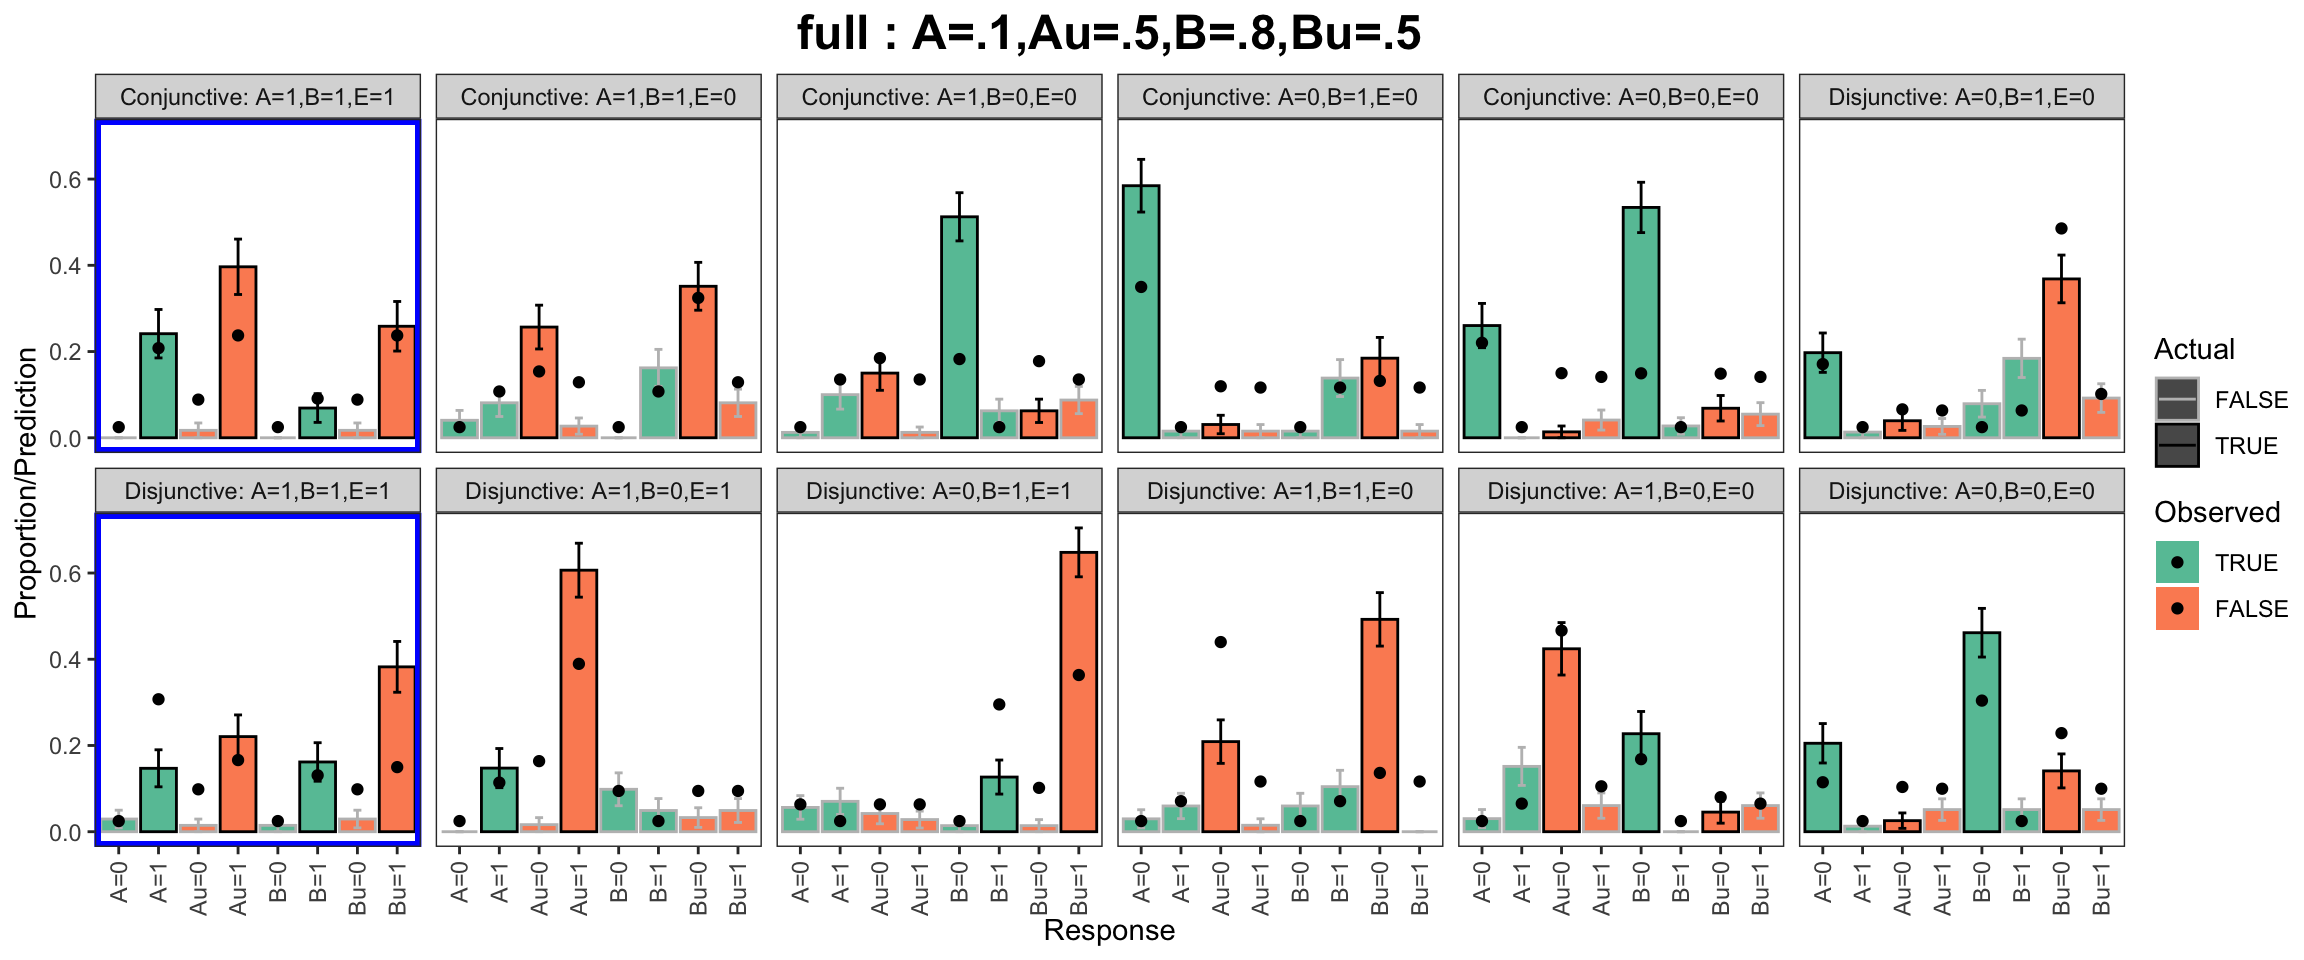
\includegraphics[keepaspectratio]{reportingFigs16m_files/figure-latex/unnamed-chunk-7-1.pdf}}
\pandocbounded{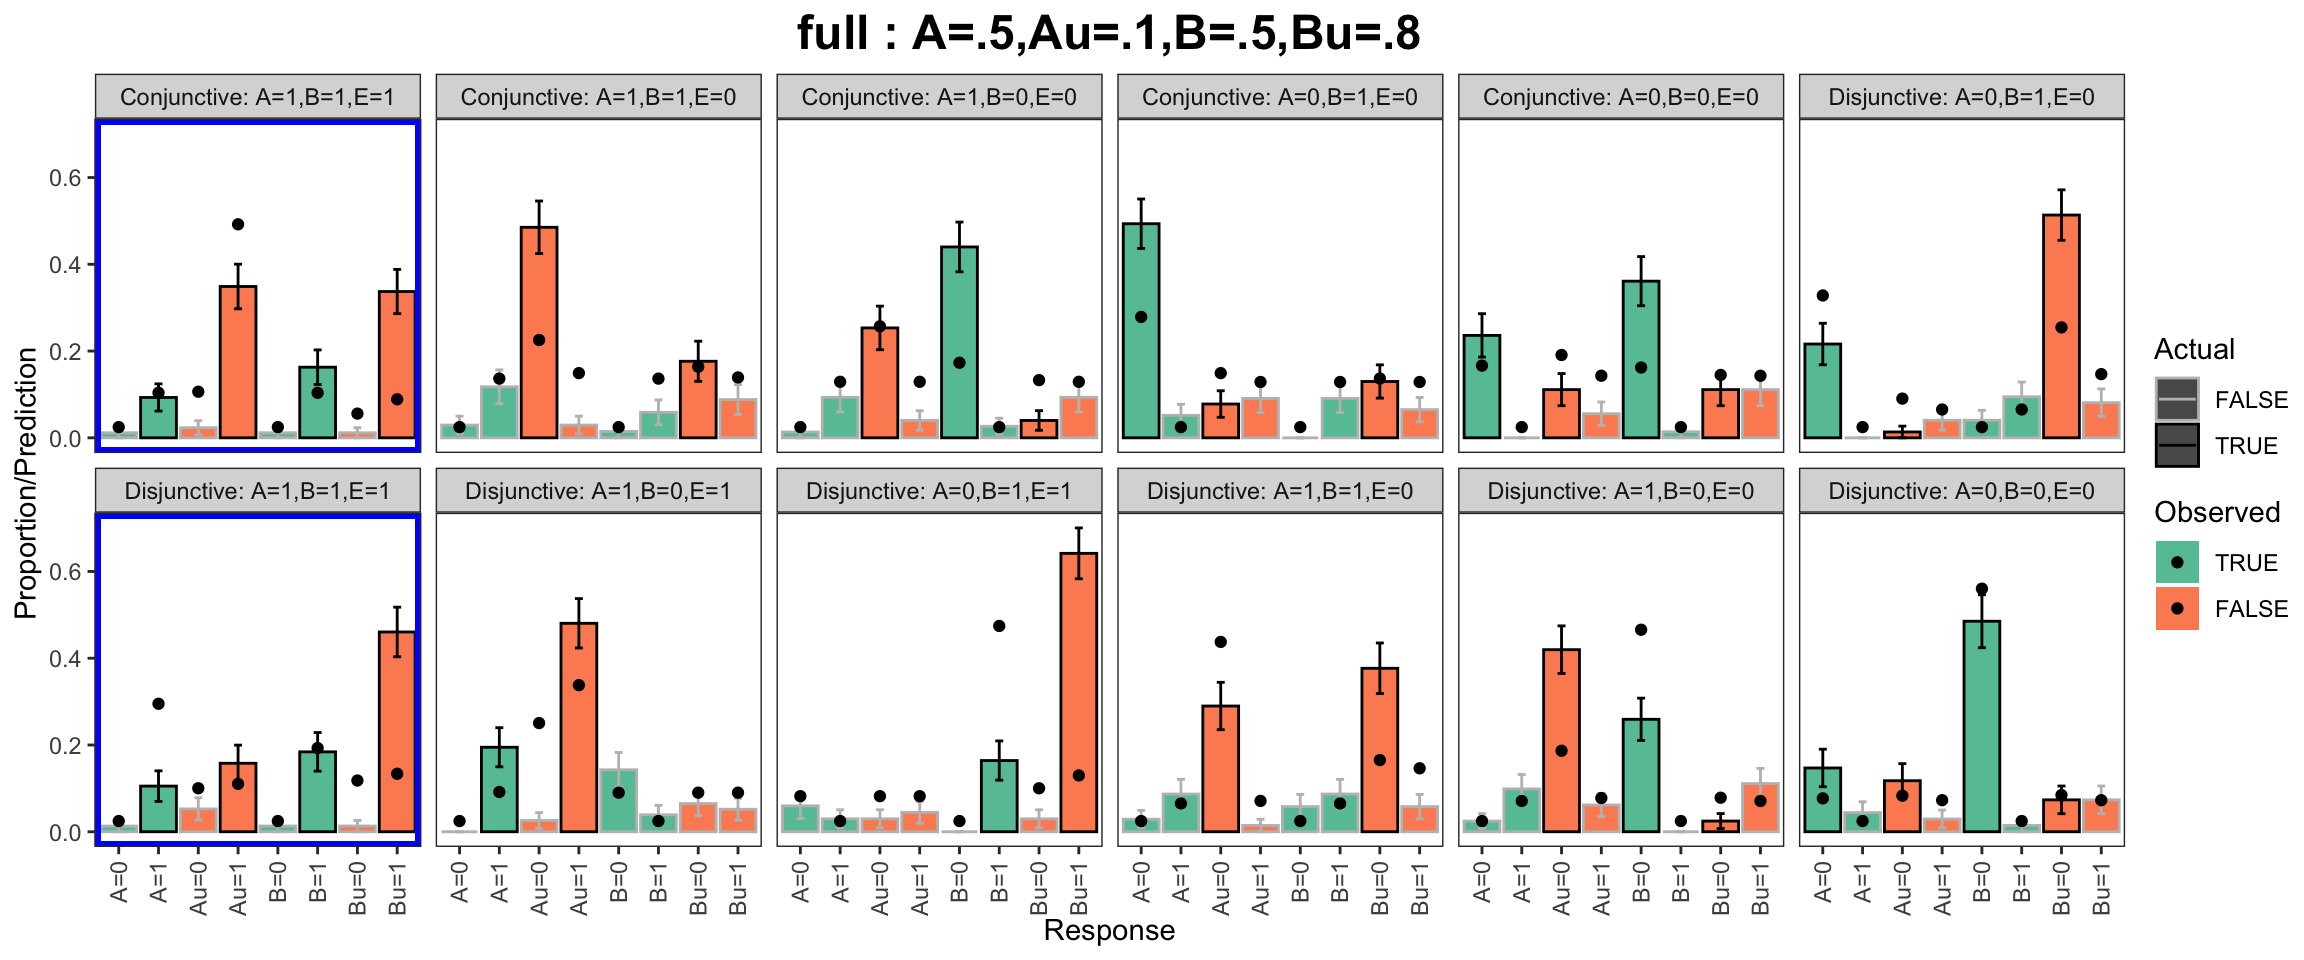
\includegraphics[keepaspectratio]{reportingFigs16m_files/figure-latex/unnamed-chunk-7-2.pdf}}
\pandocbounded{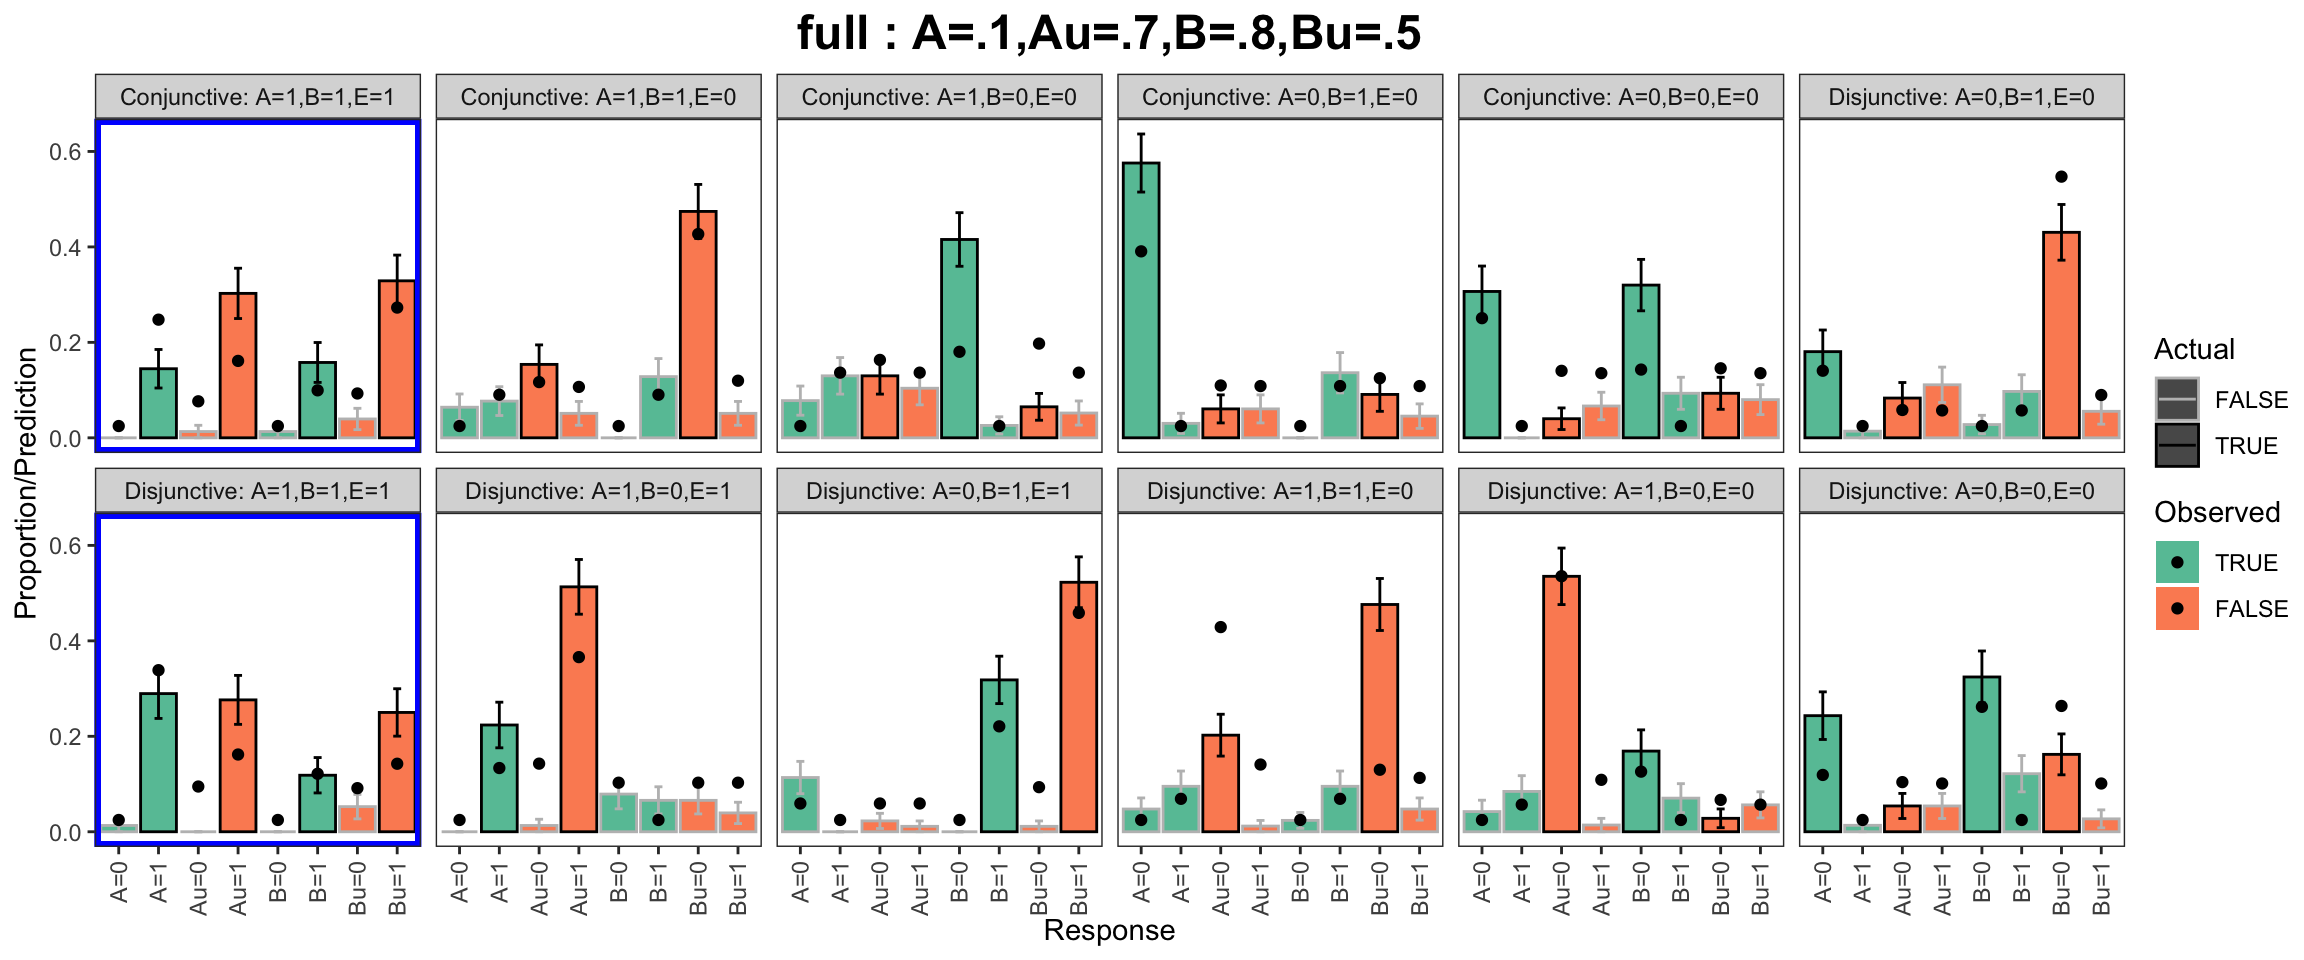
\includegraphics[keepaspectratio]{reportingFigs16m_files/figure-latex/unnamed-chunk-7-3.pdf}}
\pandocbounded{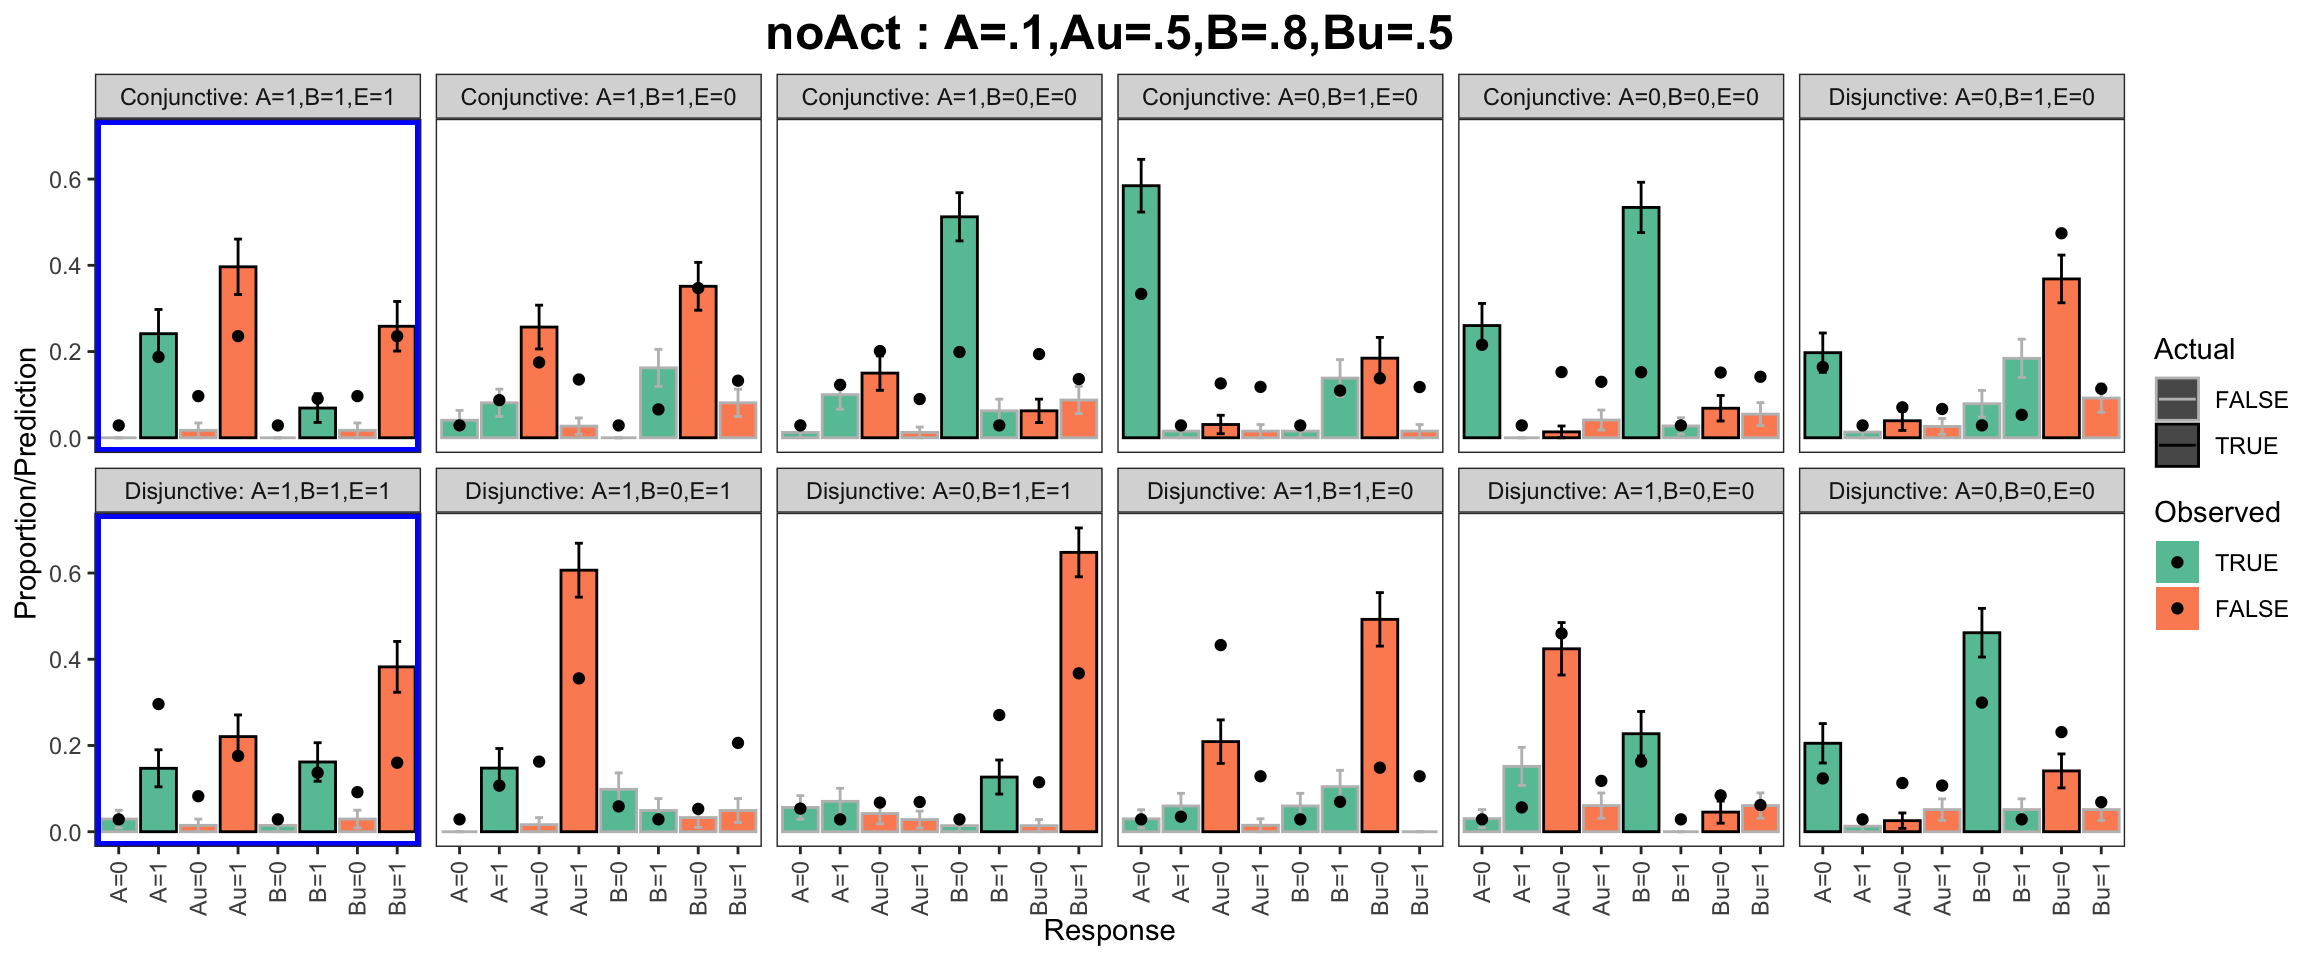
\includegraphics[keepaspectratio]{reportingFigs16m_files/figure-latex/unnamed-chunk-7-4.pdf}}
\pandocbounded{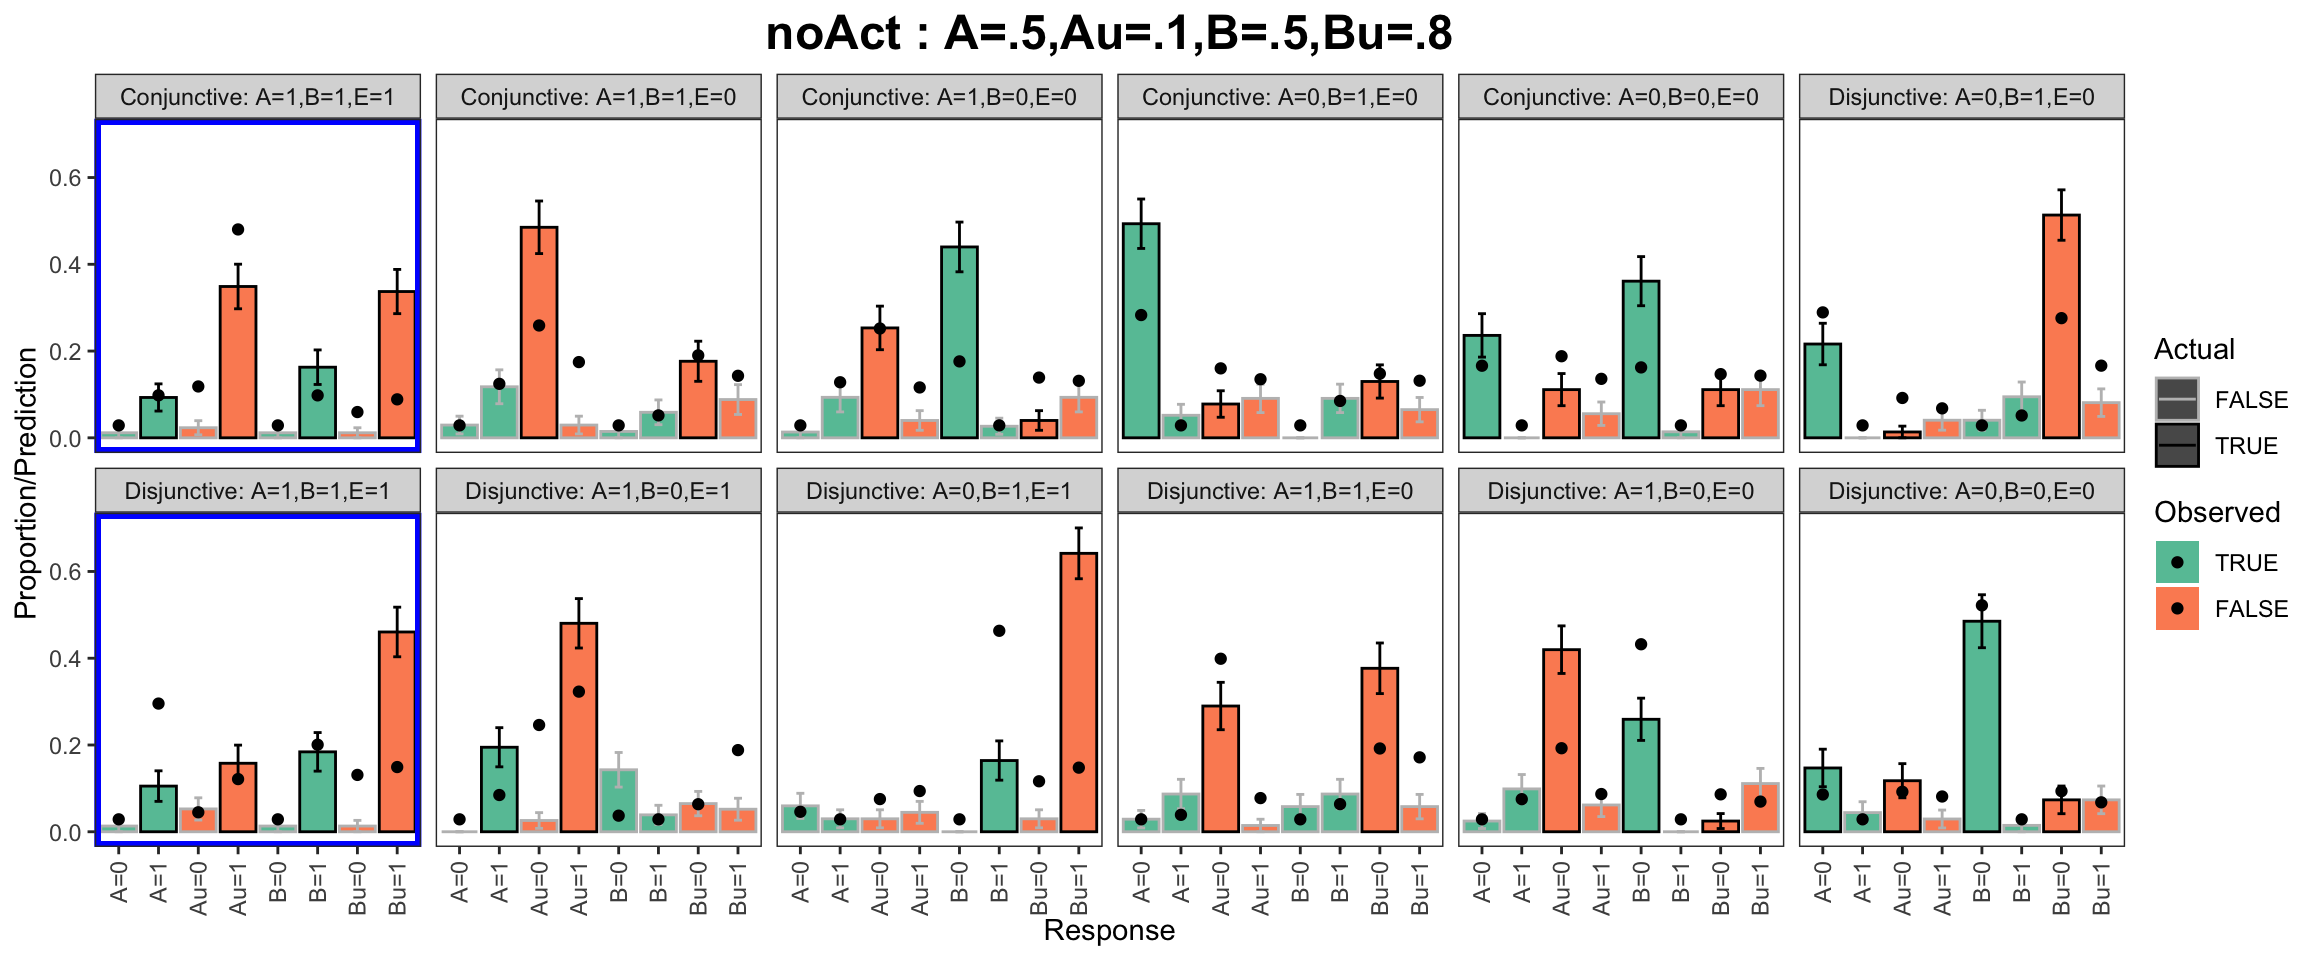
\includegraphics[keepaspectratio]{reportingFigs16m_files/figure-latex/unnamed-chunk-7-5.pdf}}
\pandocbounded{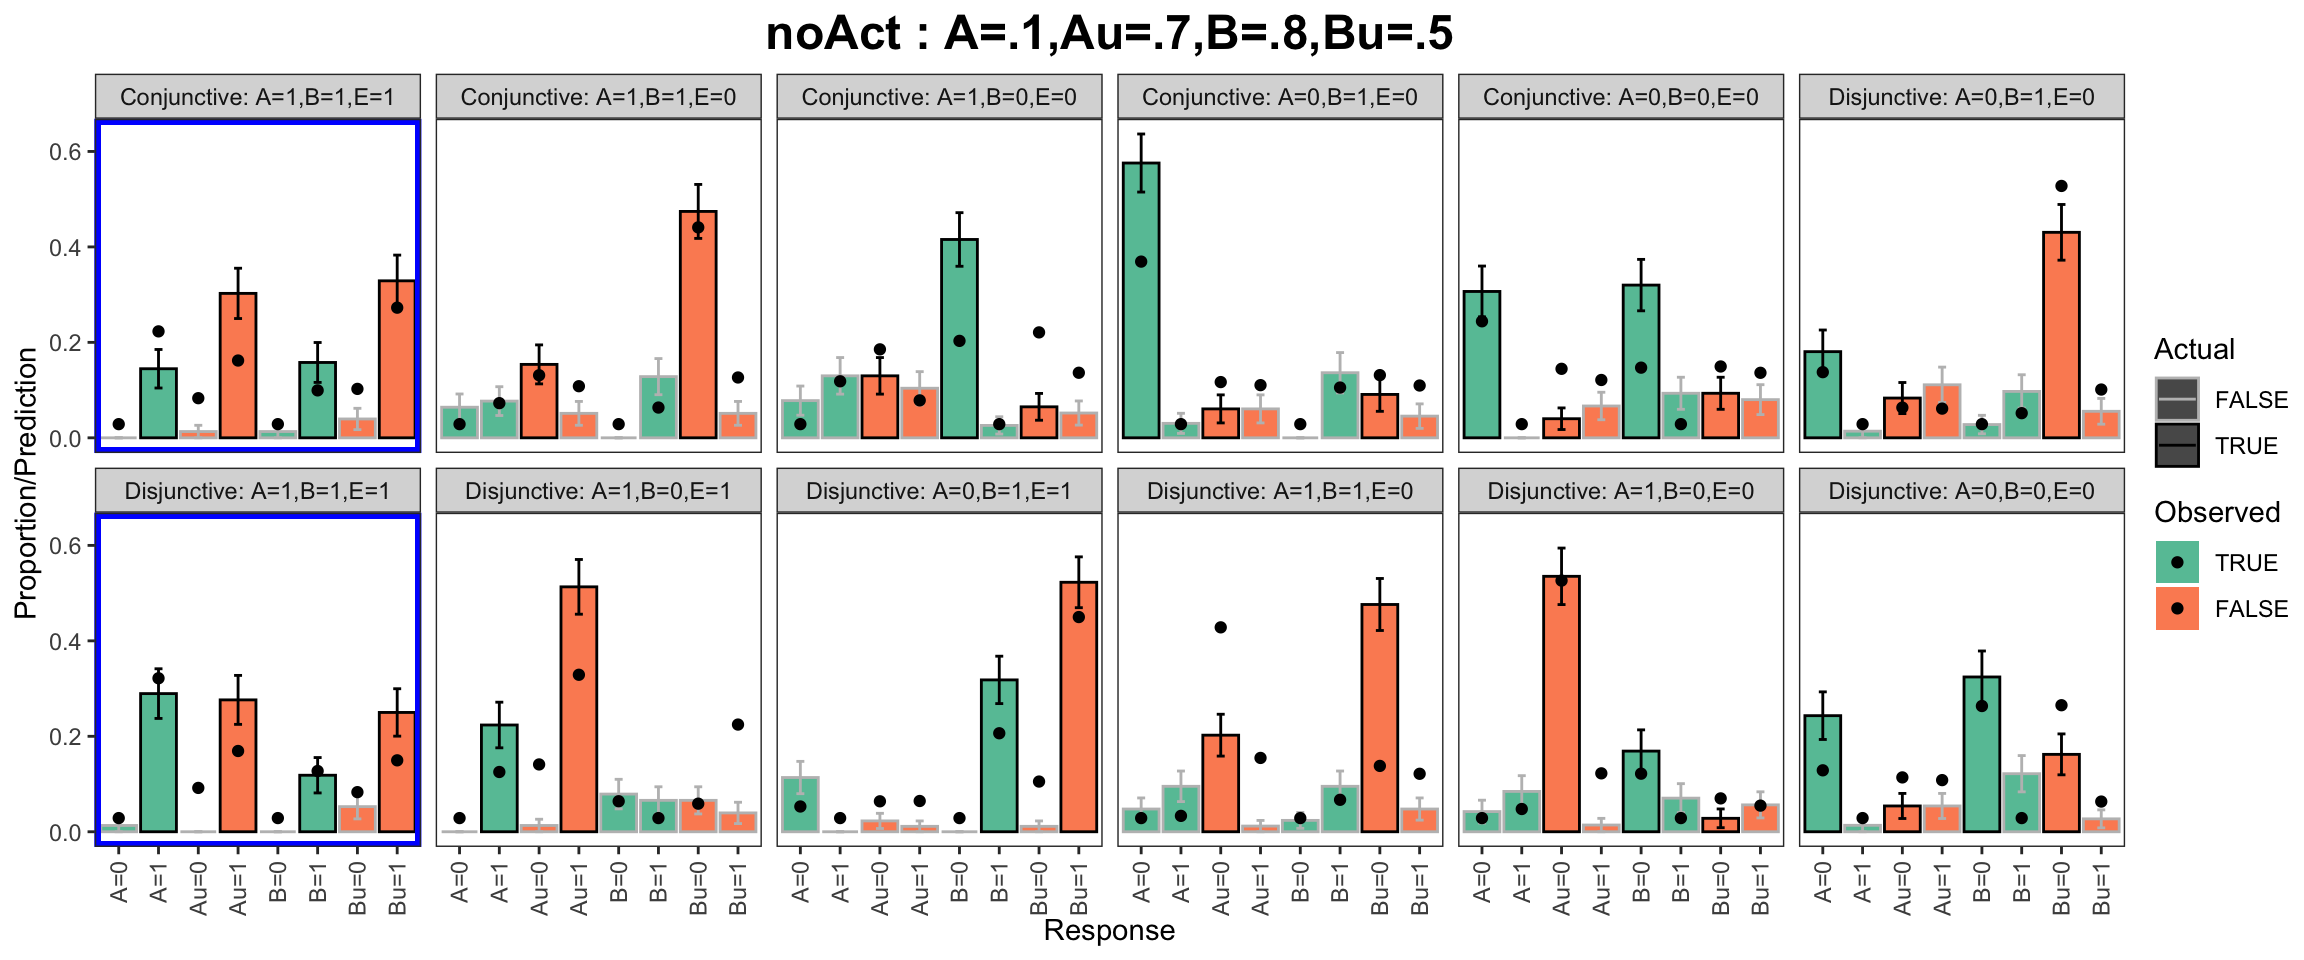
\includegraphics[keepaspectratio]{reportingFigs16m_files/figure-latex/unnamed-chunk-7-6.pdf}}
\pandocbounded{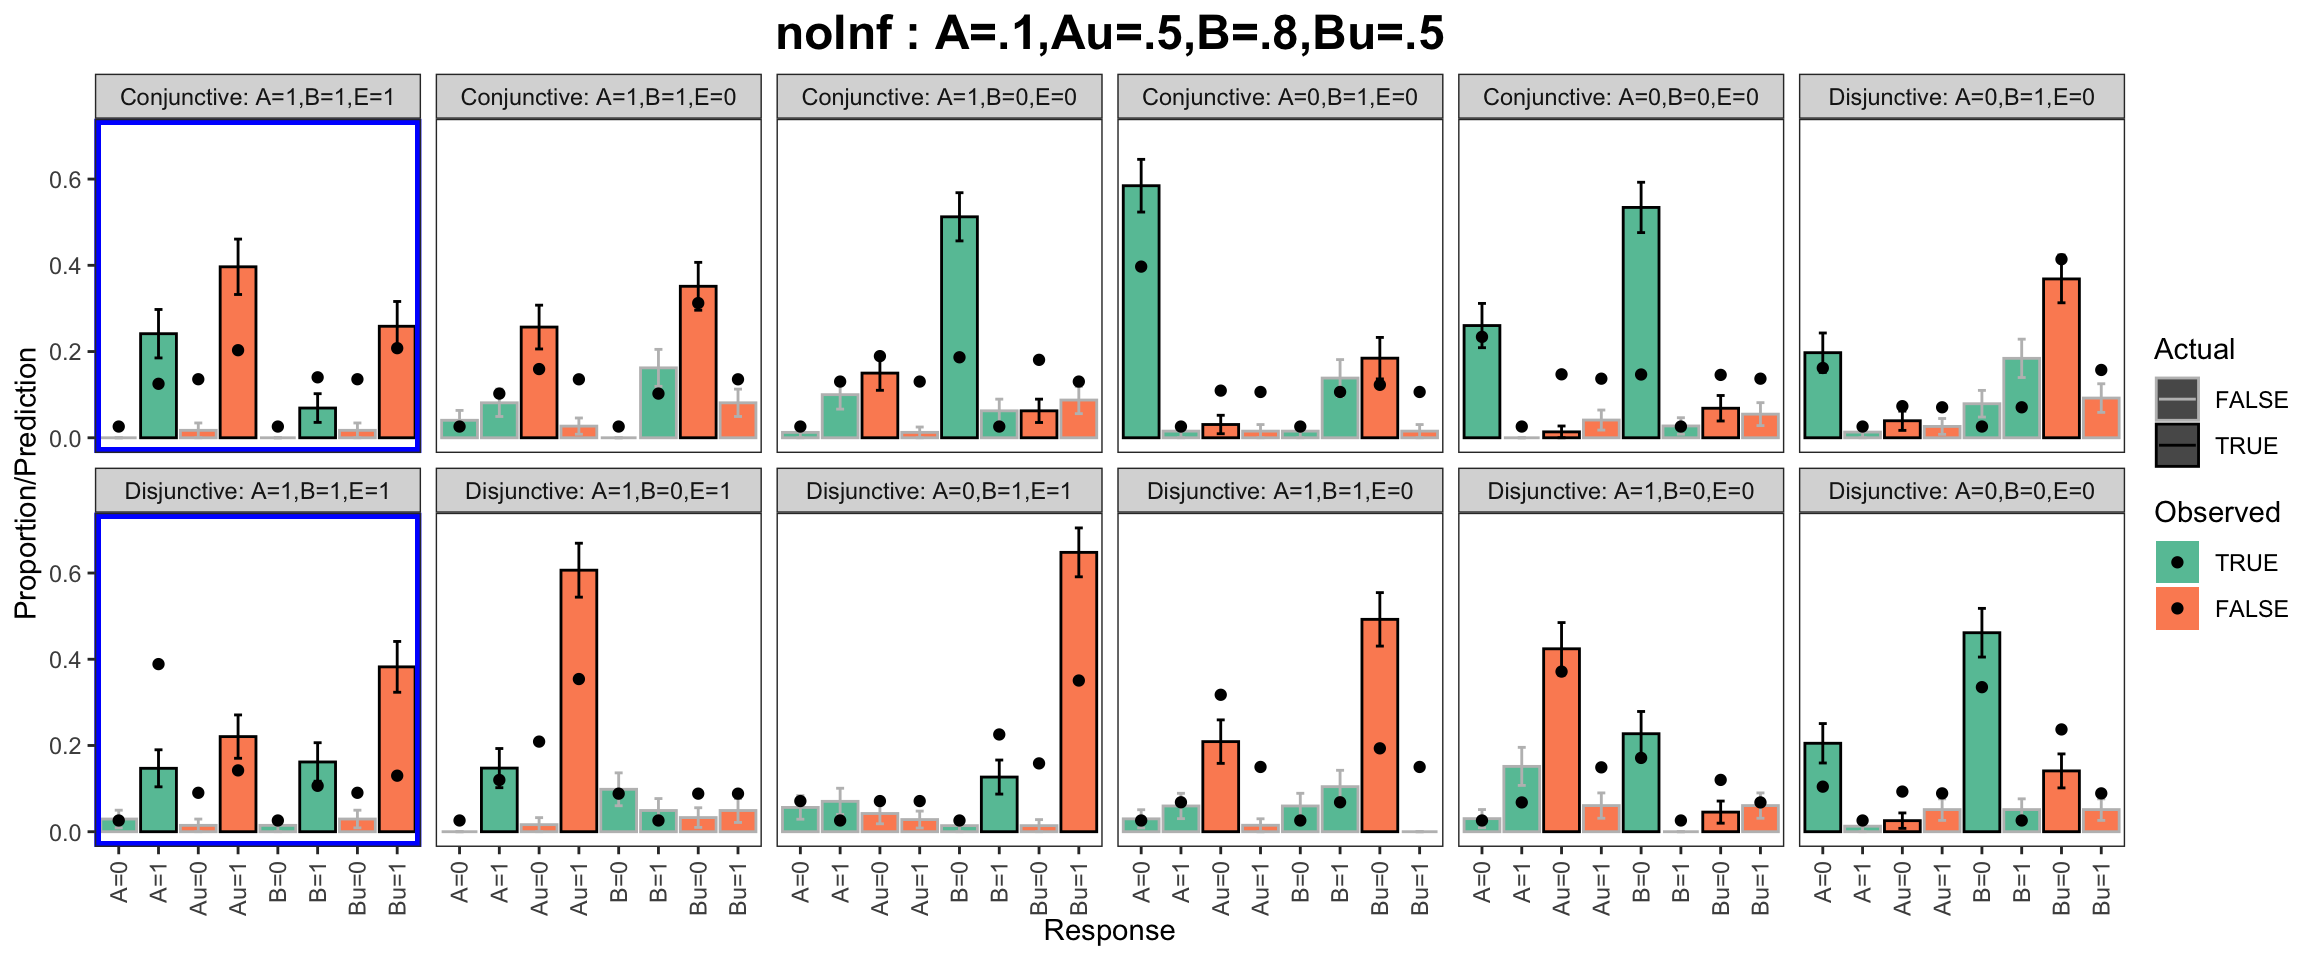
\includegraphics[keepaspectratio]{reportingFigs16m_files/figure-latex/unnamed-chunk-7-7.pdf}}
\pandocbounded{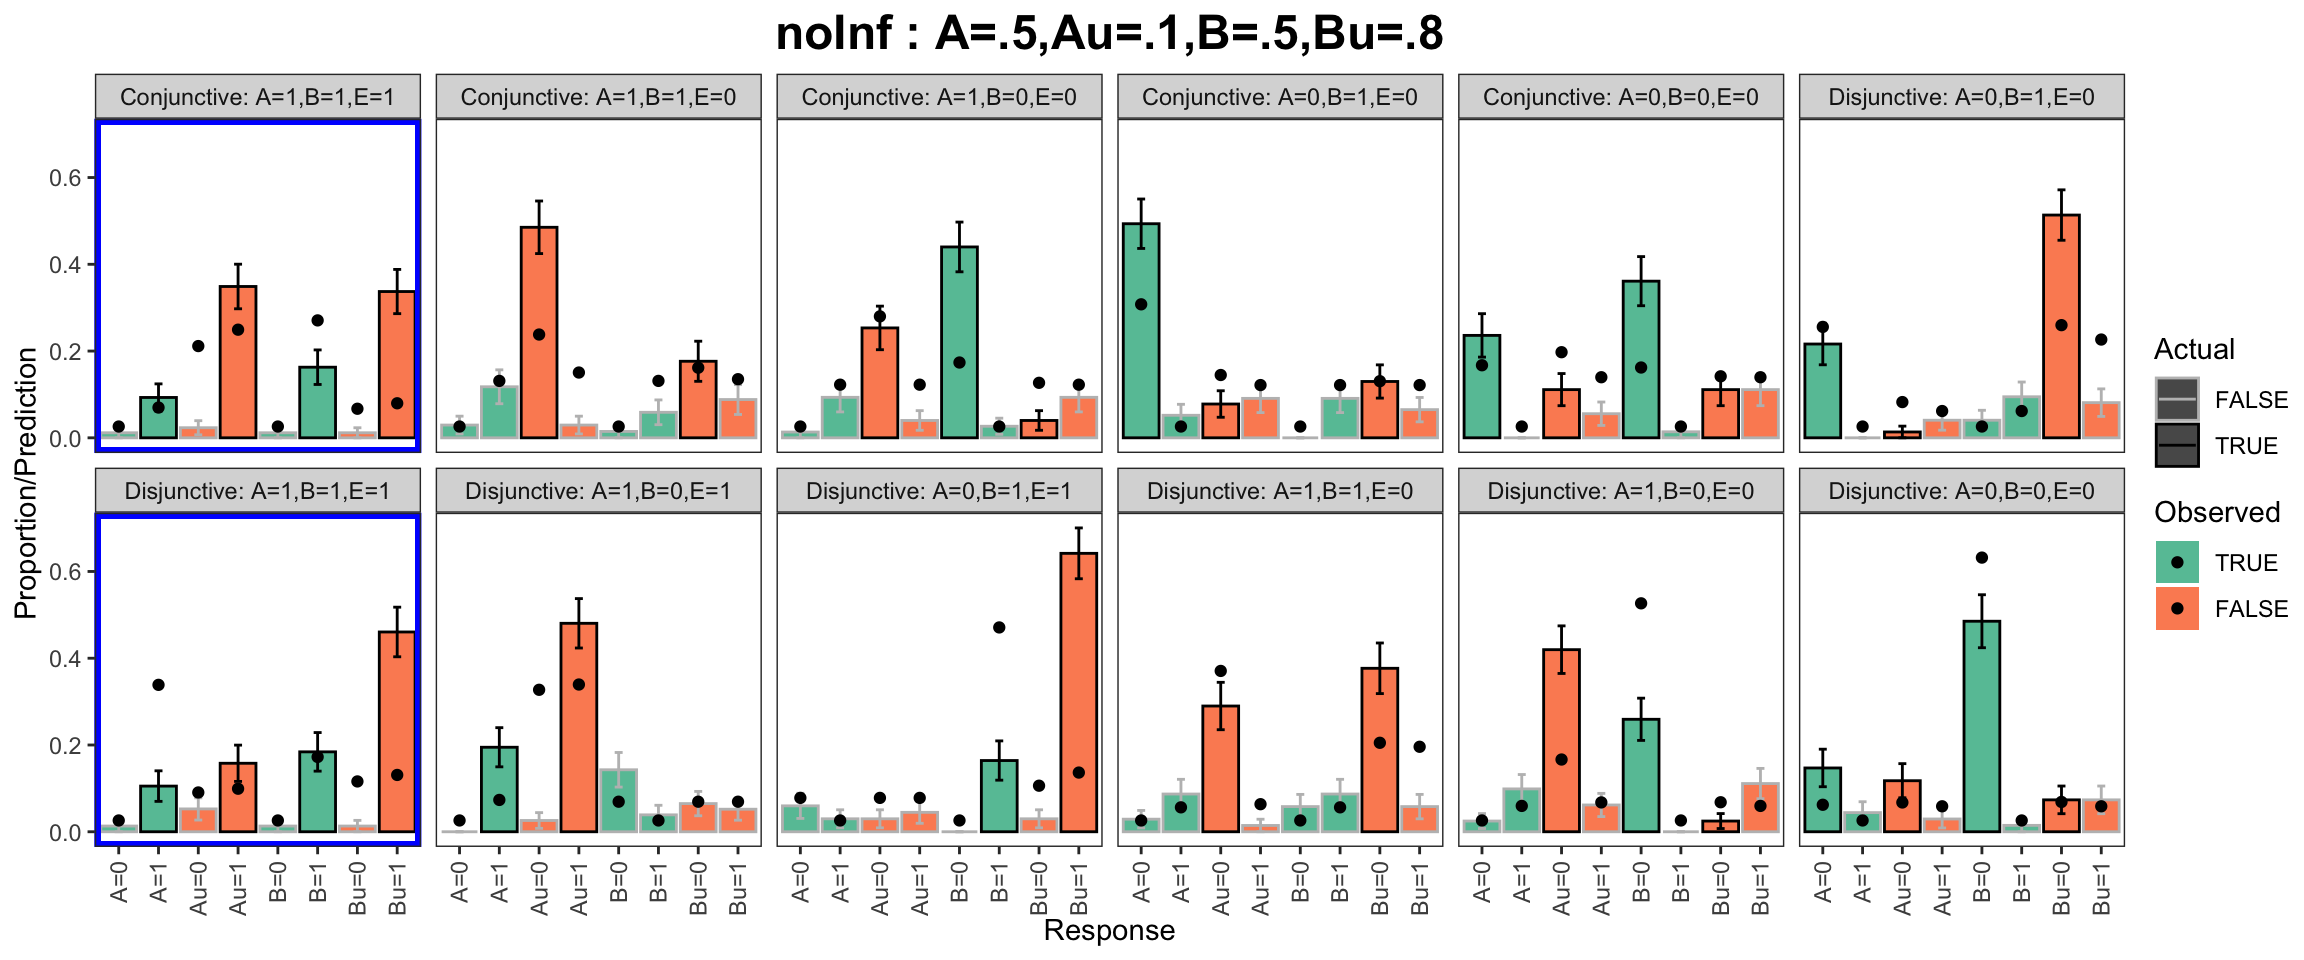
\includegraphics[keepaspectratio]{reportingFigs16m_files/figure-latex/unnamed-chunk-7-8.pdf}}
\pandocbounded{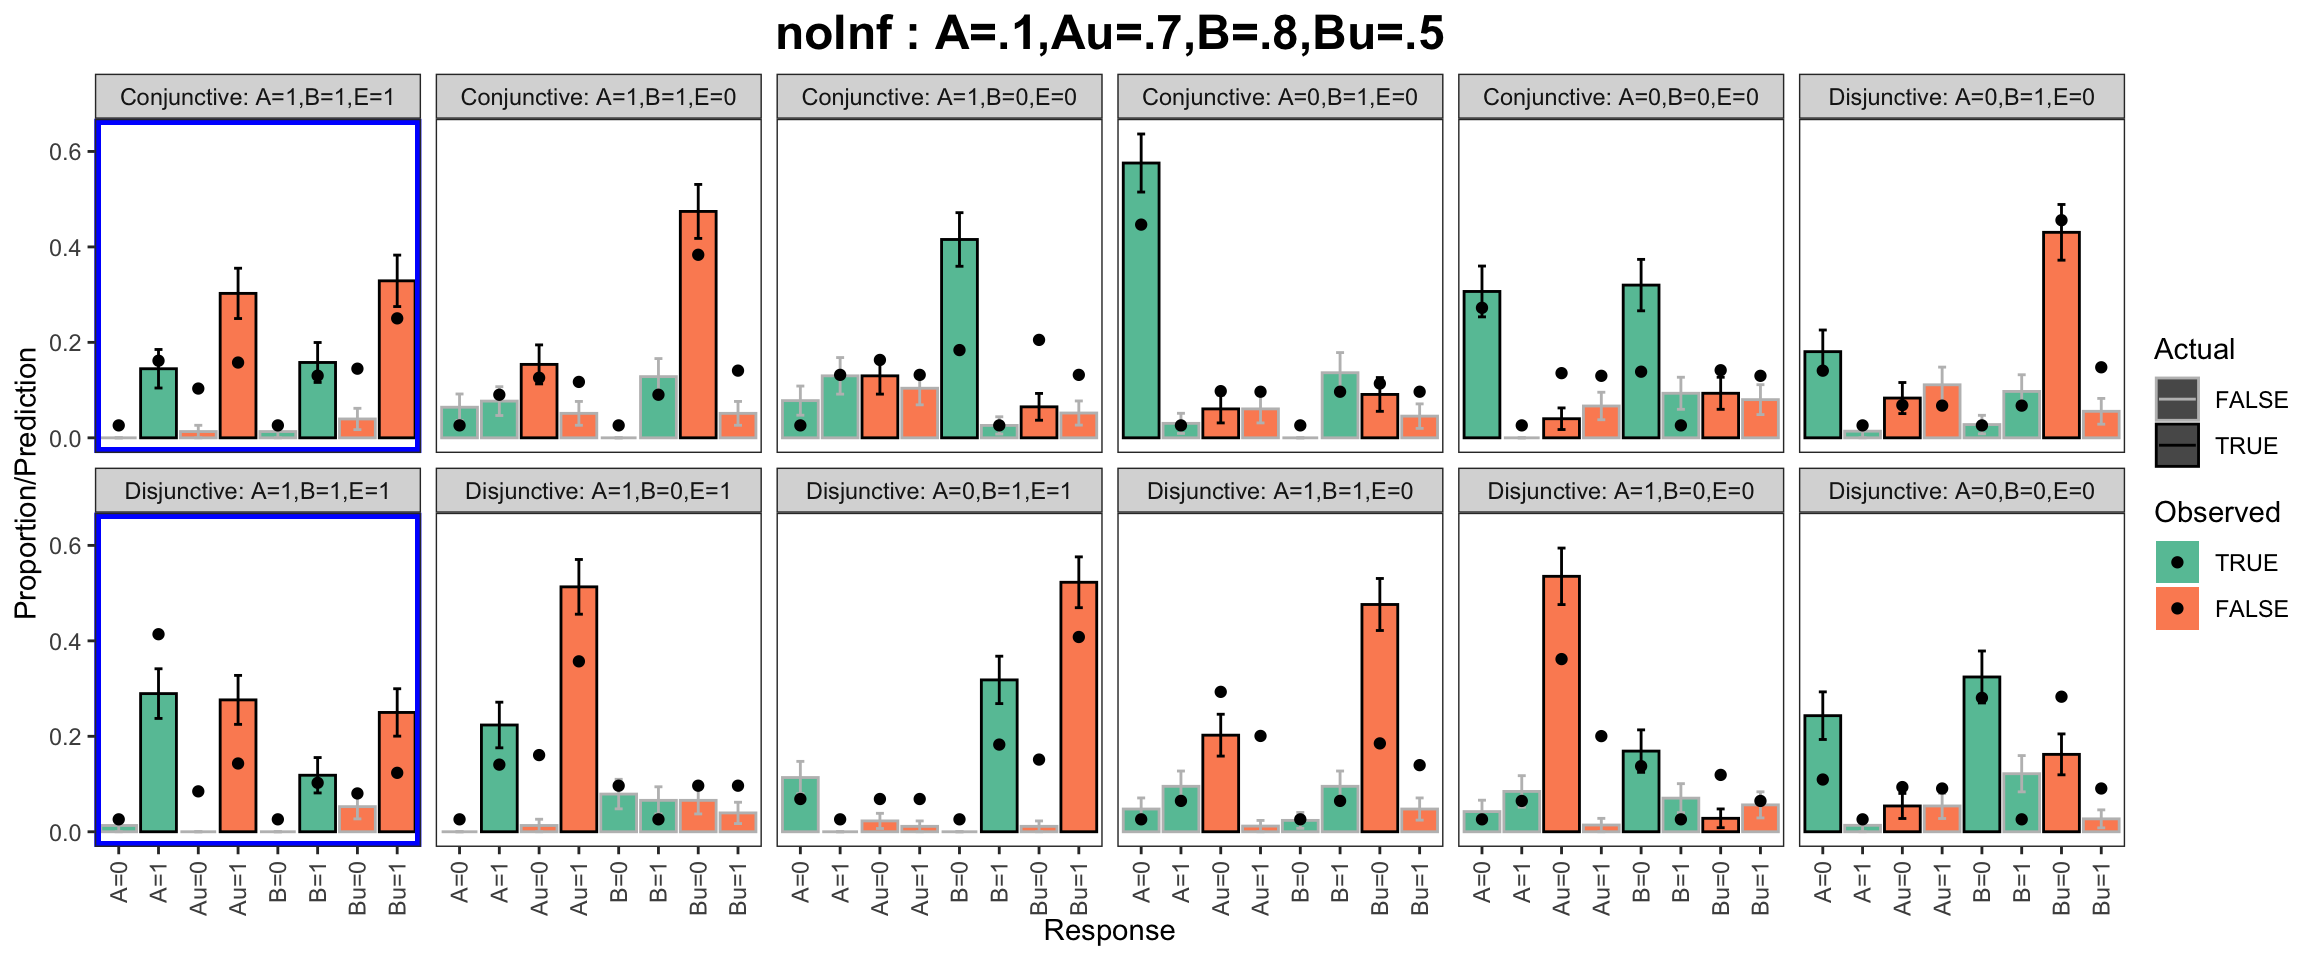
\includegraphics[keepaspectratio]{reportingFigs16m_files/figure-latex/unnamed-chunk-7-9.pdf}}
\pandocbounded{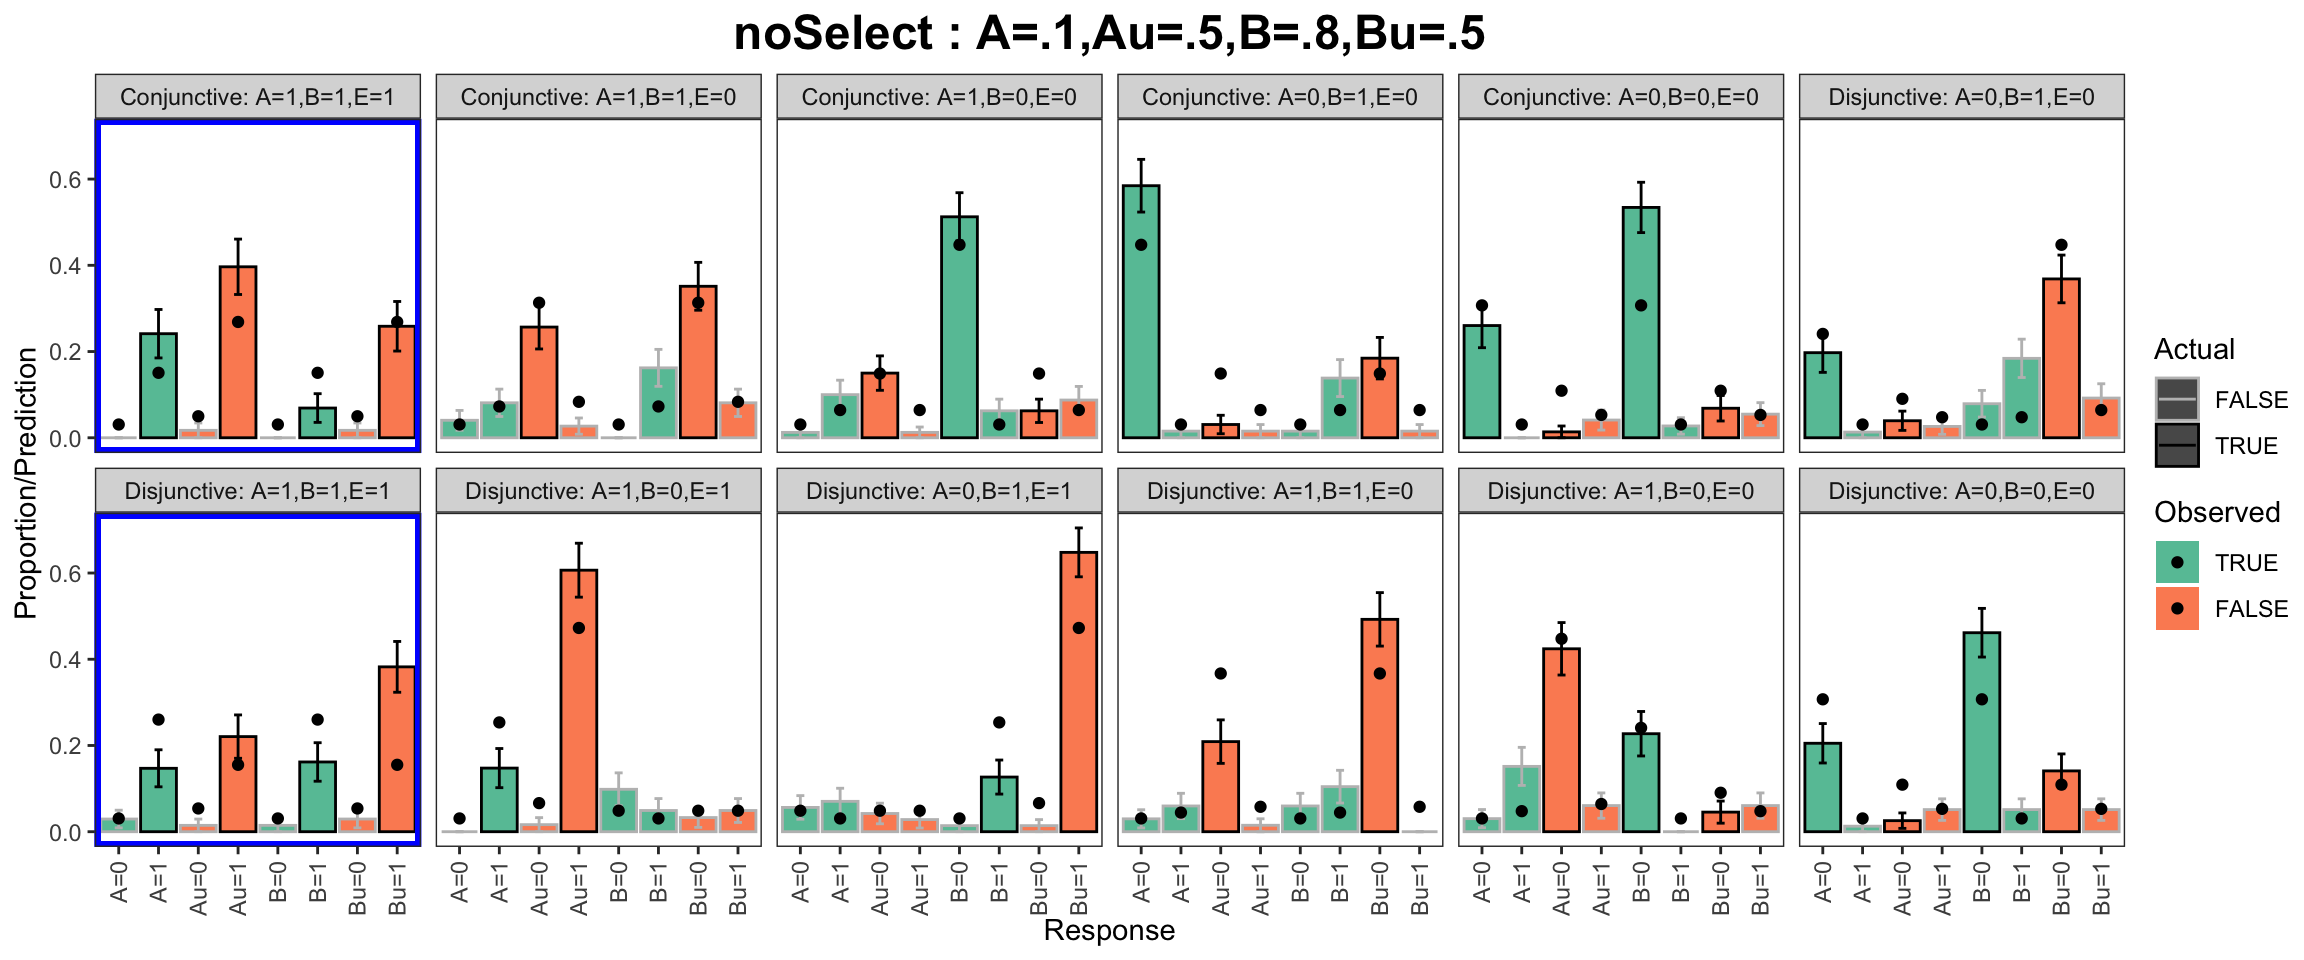
\includegraphics[keepaspectratio]{reportingFigs16m_files/figure-latex/unnamed-chunk-7-10.pdf}}
\pandocbounded{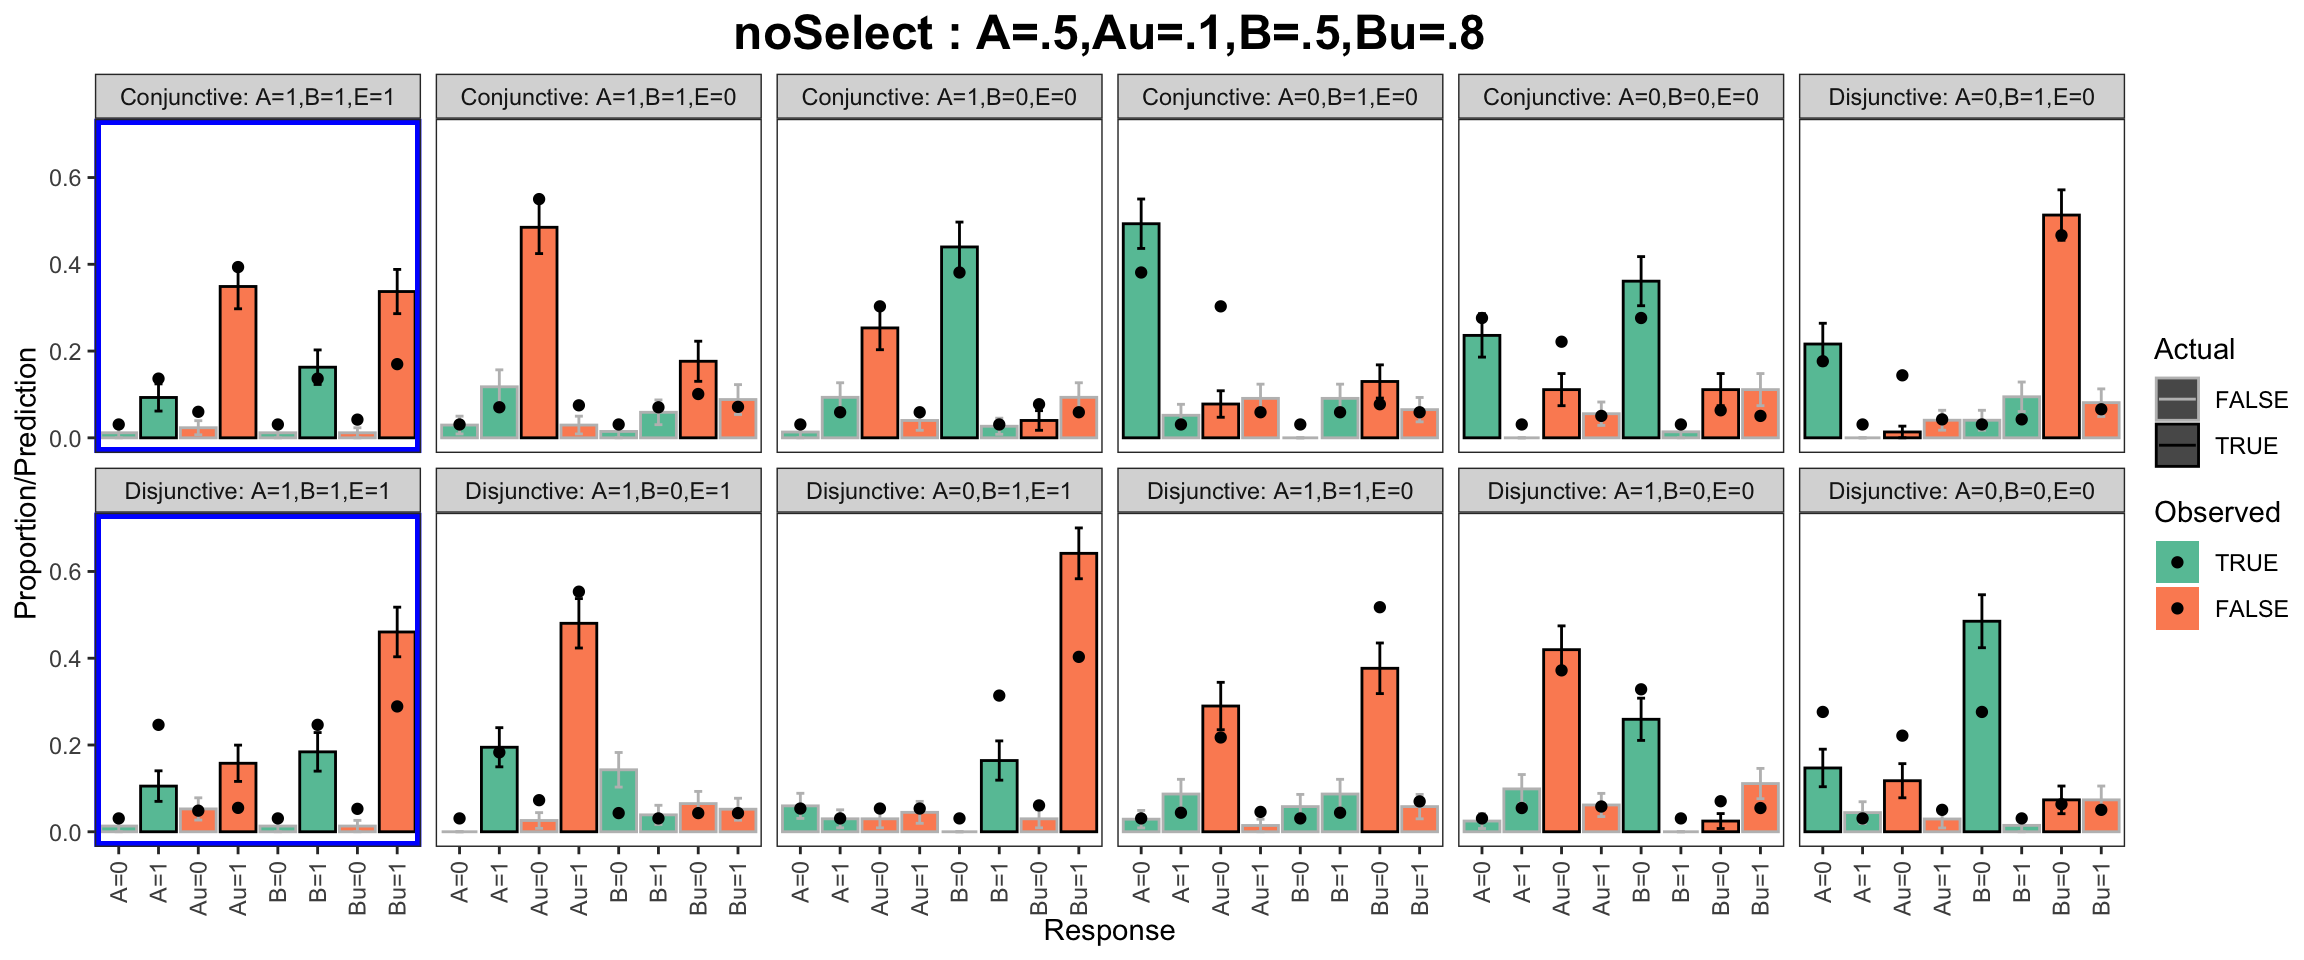
\includegraphics[keepaspectratio]{reportingFigs16m_files/figure-latex/unnamed-chunk-7-11.pdf}}
\pandocbounded{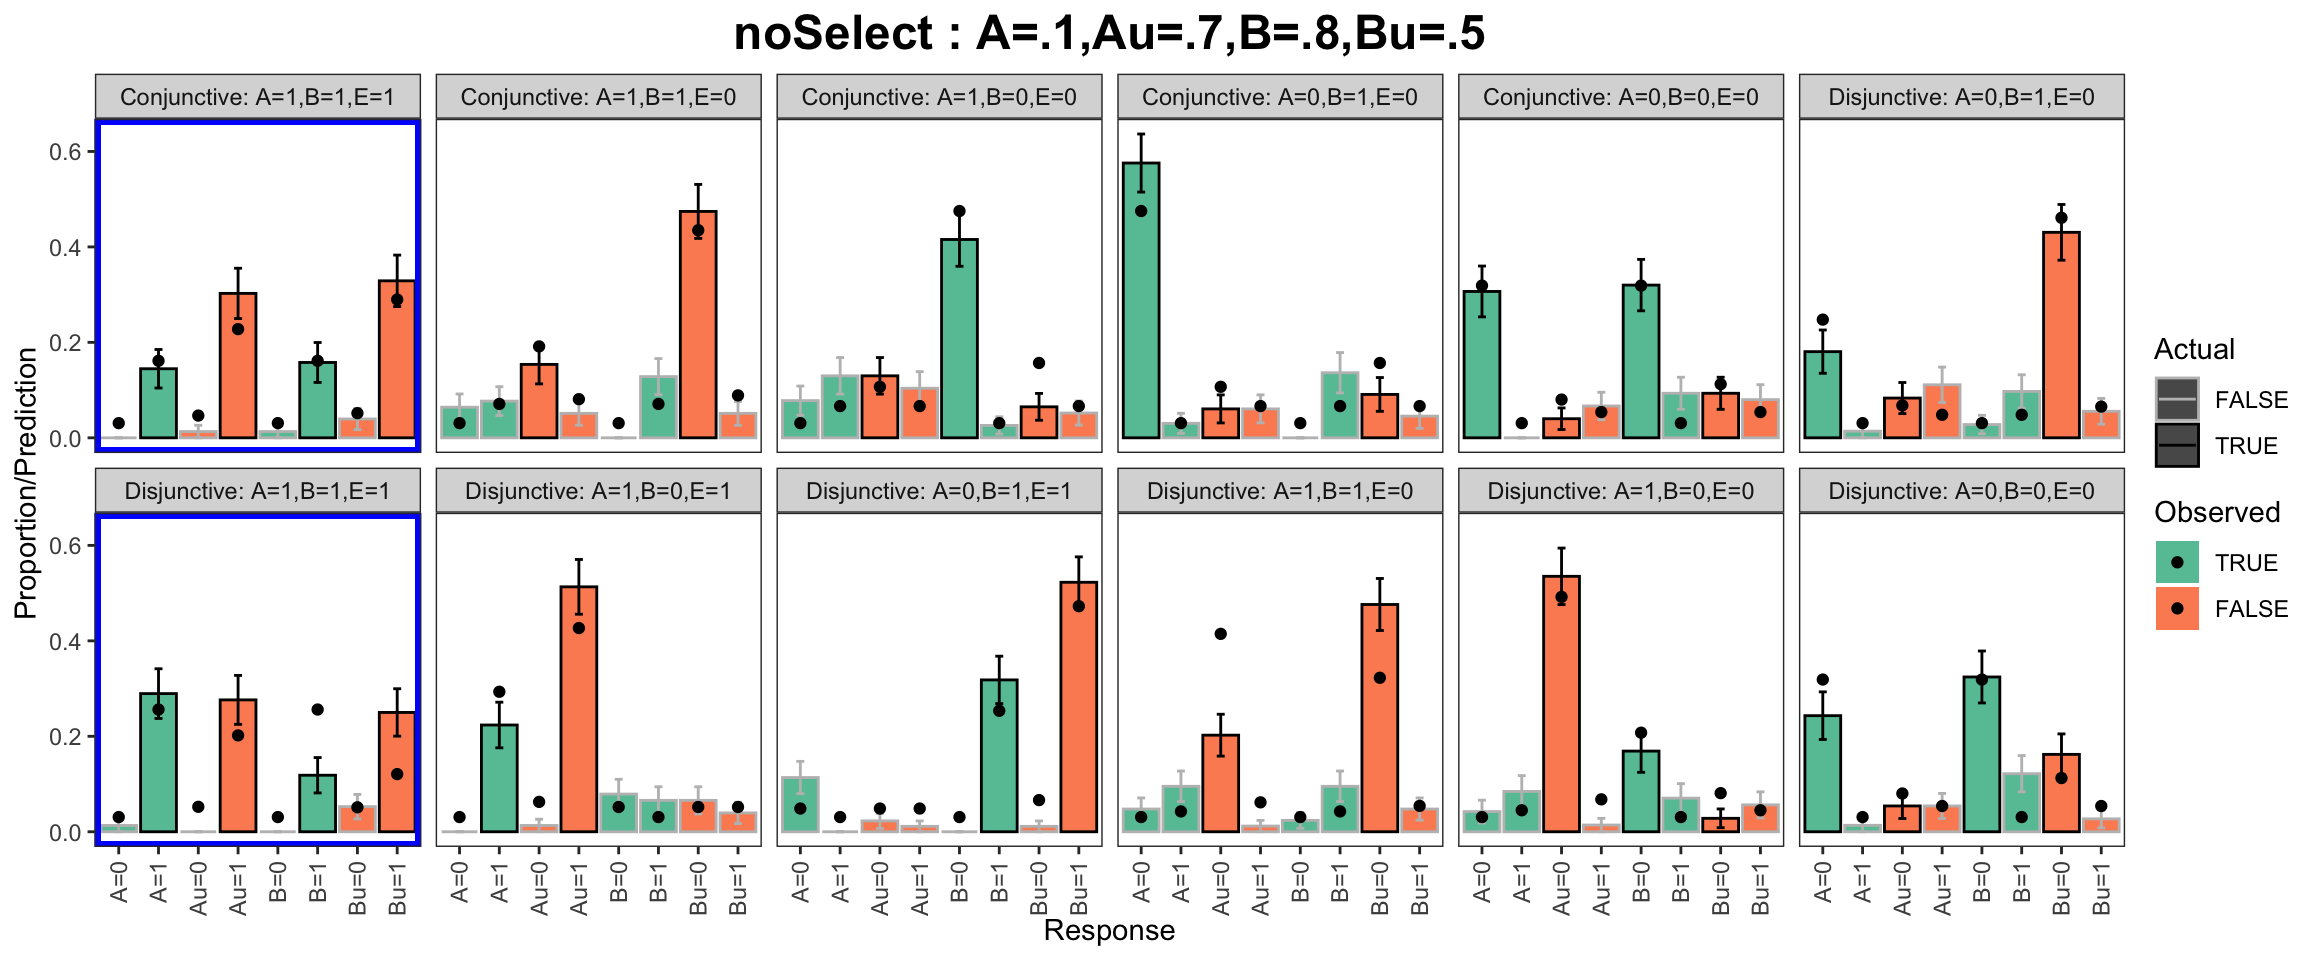
\includegraphics[keepaspectratio]{reportingFigs16m_files/figure-latex/unnamed-chunk-7-12.pdf}}
\pandocbounded{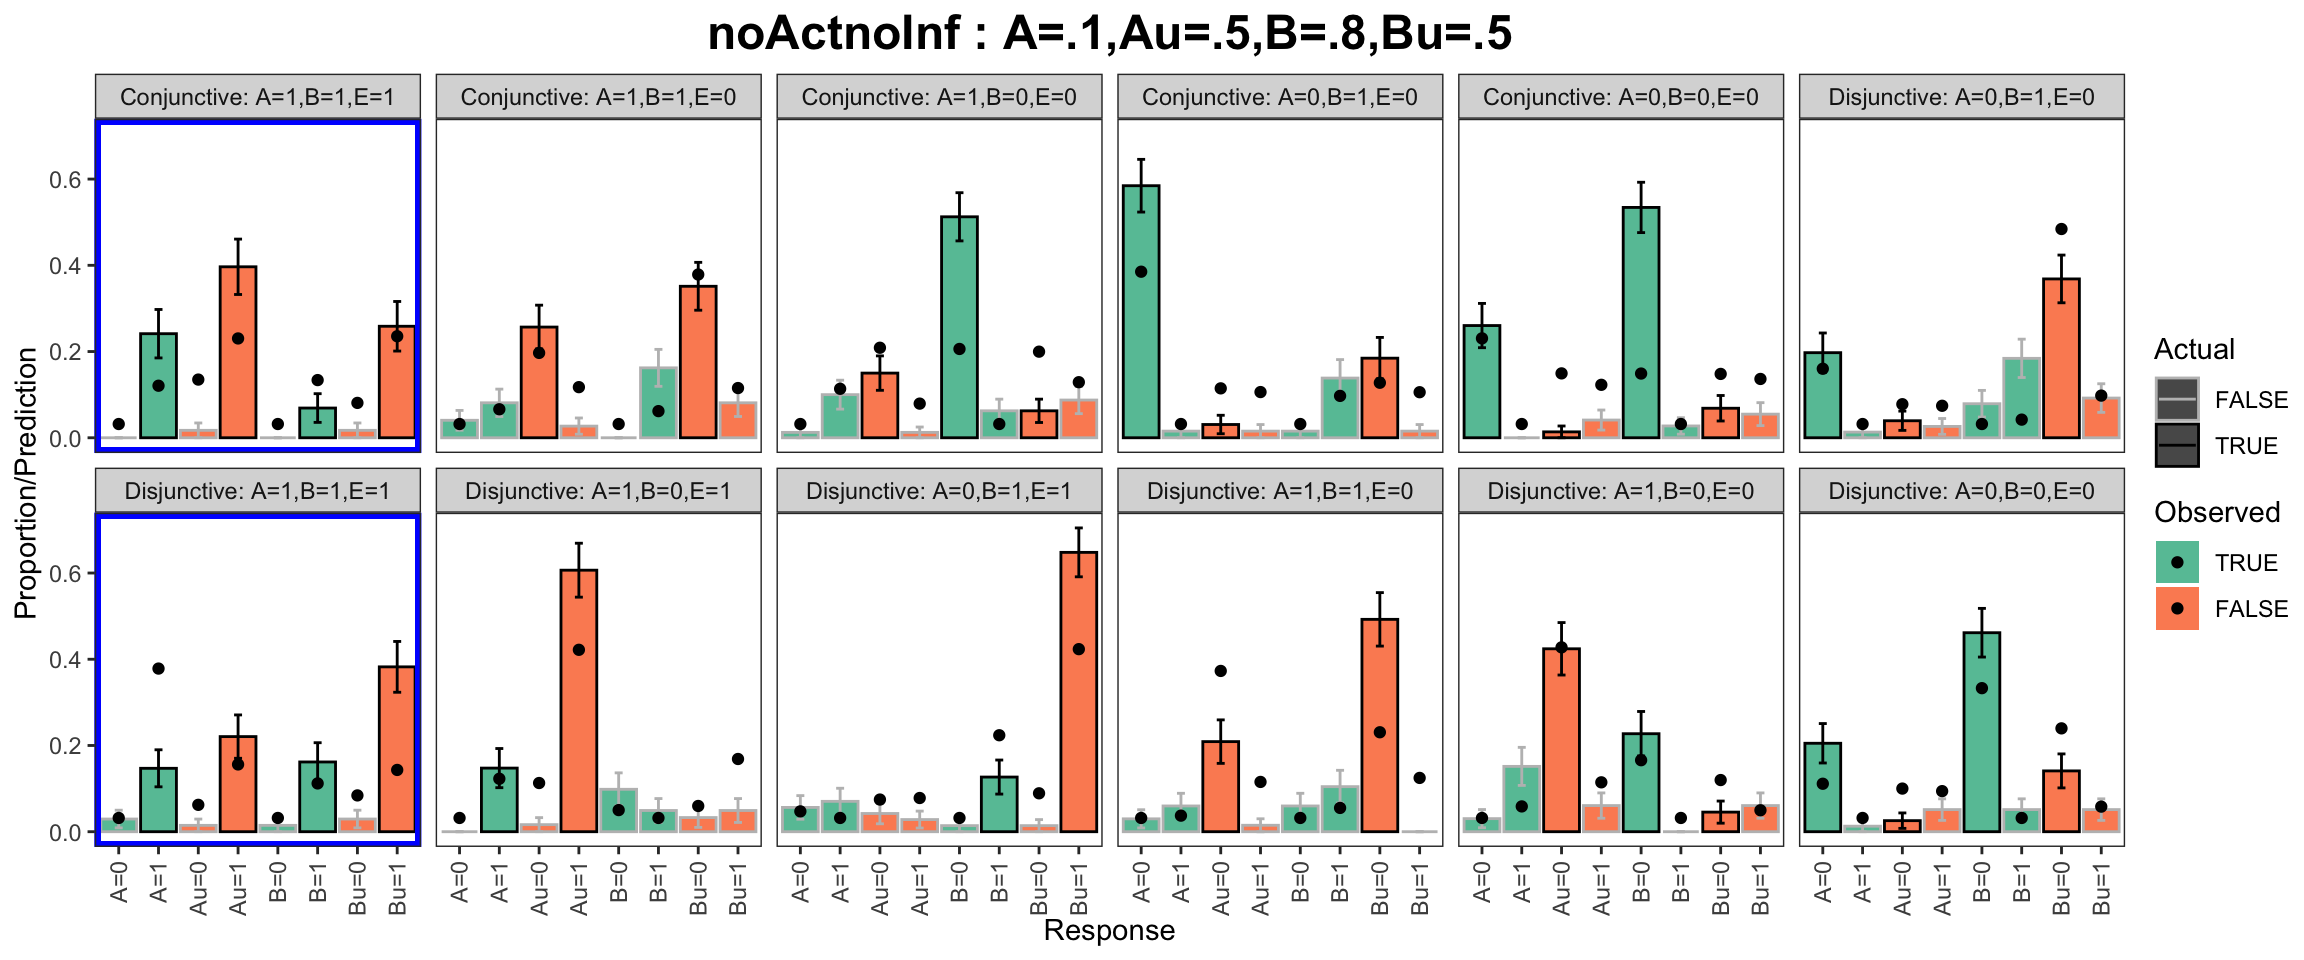
\includegraphics[keepaspectratio]{reportingFigs16m_files/figure-latex/unnamed-chunk-7-13.pdf}}
\pandocbounded{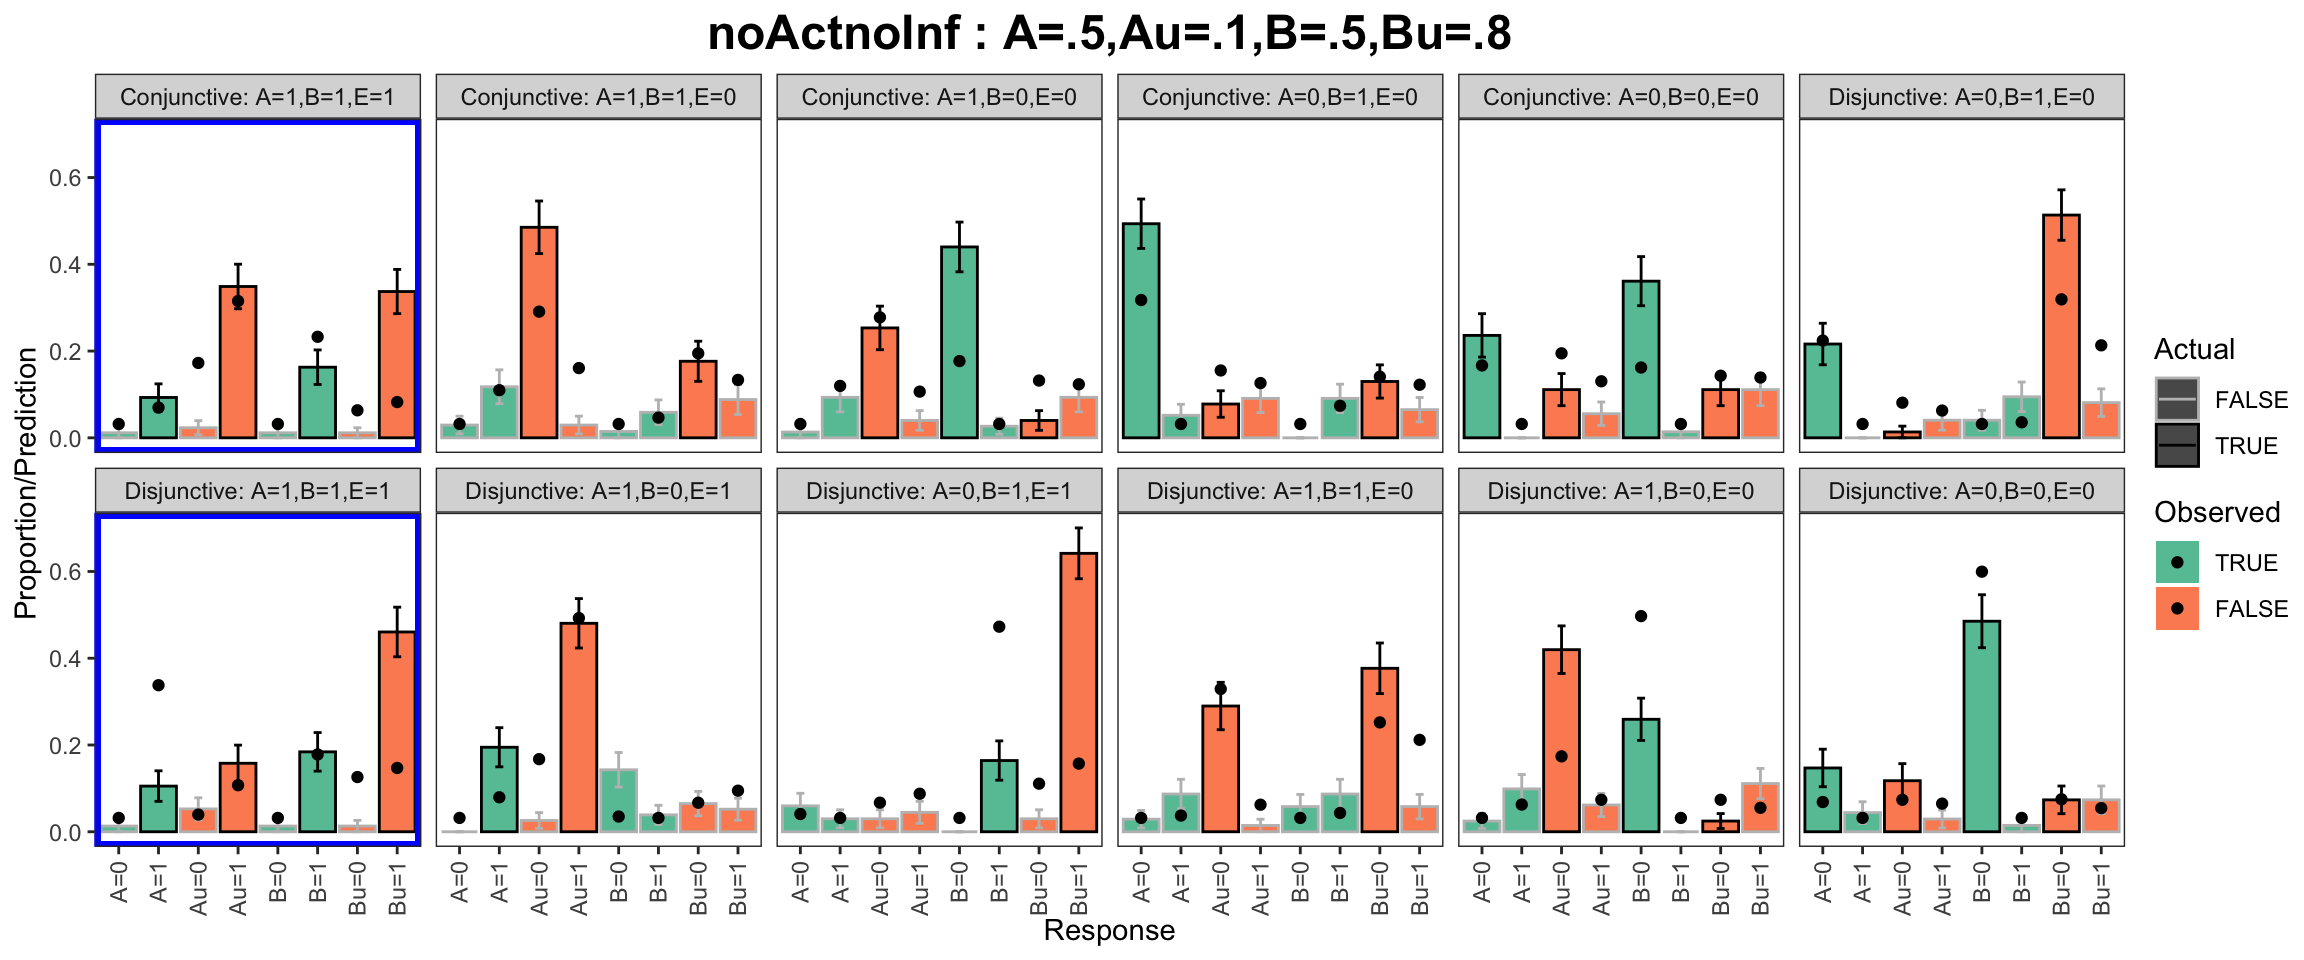
\includegraphics[keepaspectratio]{reportingFigs16m_files/figure-latex/unnamed-chunk-7-14.pdf}}
\pandocbounded{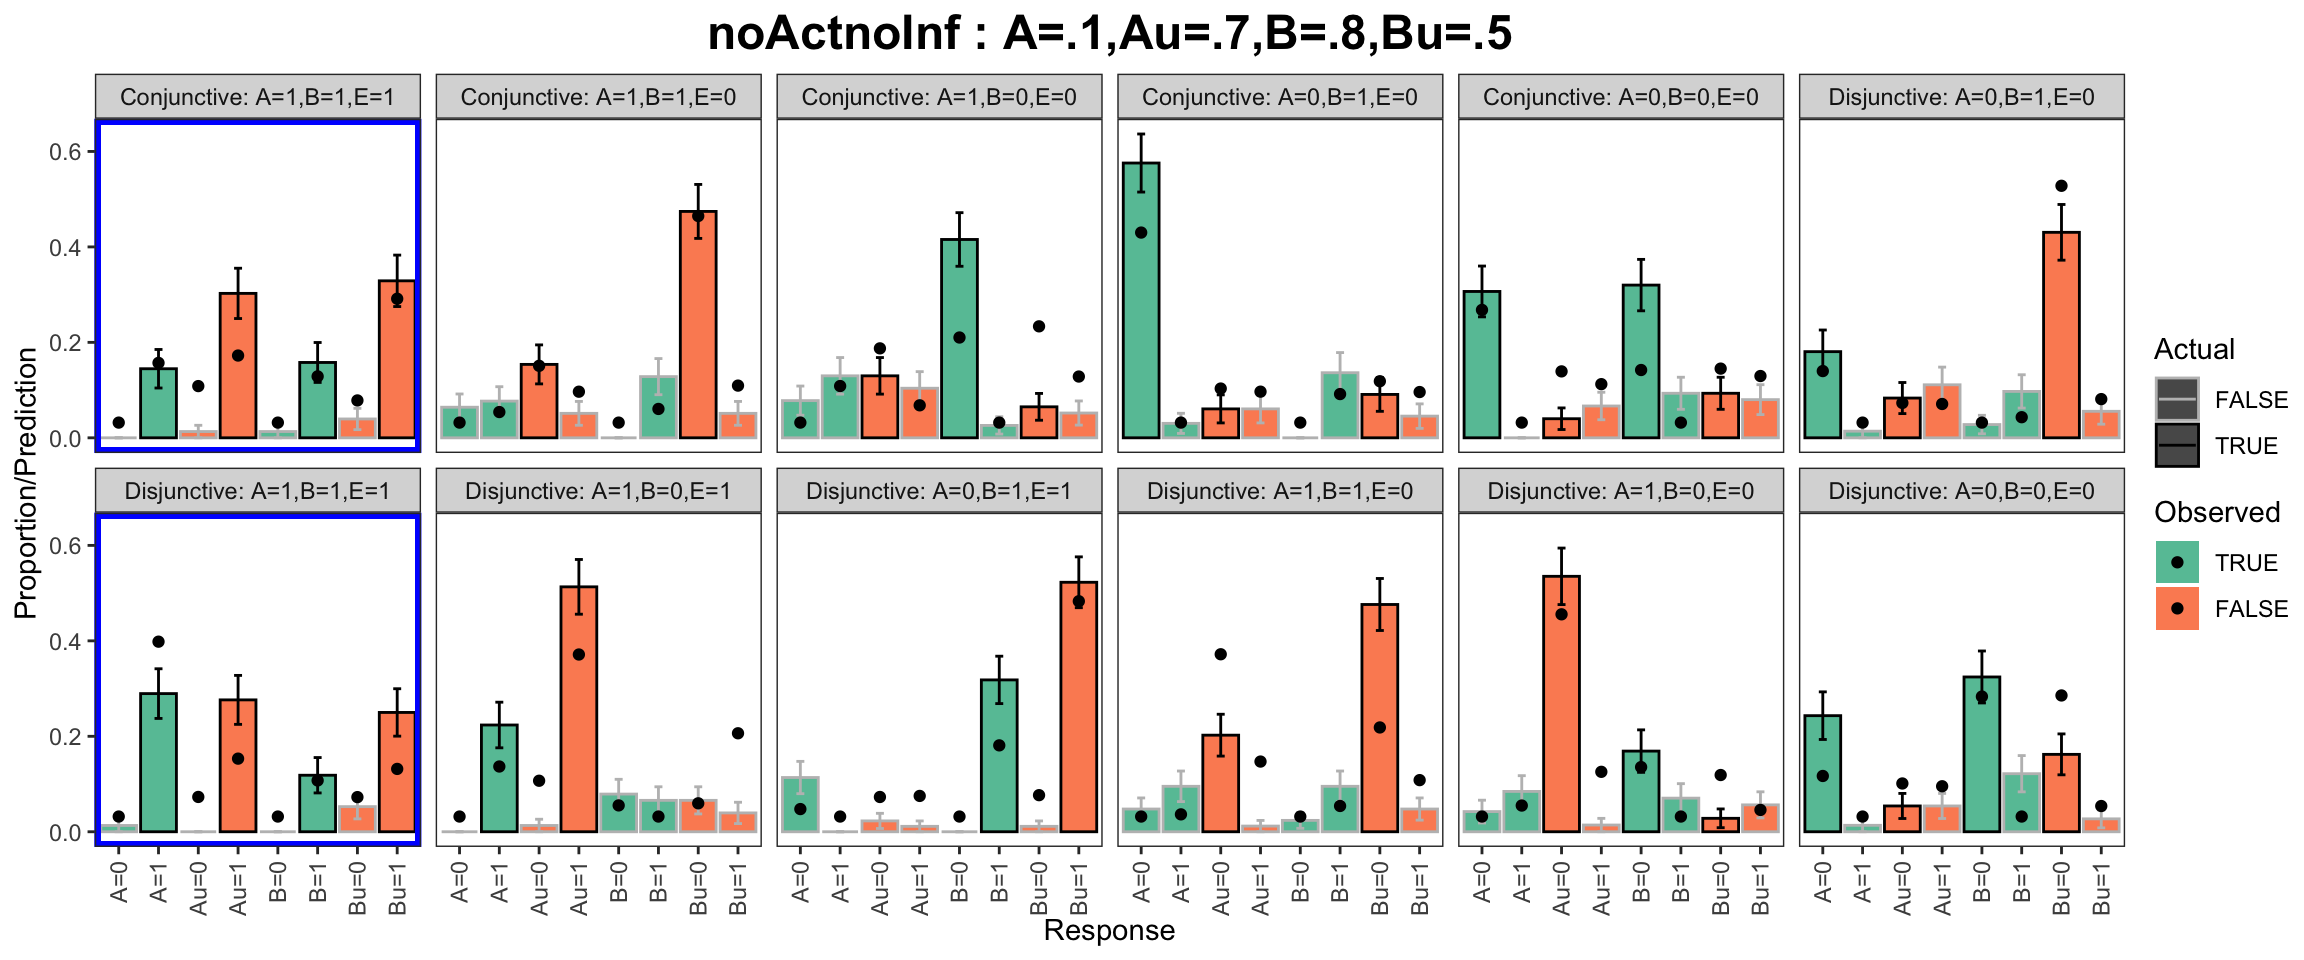
\includegraphics[keepaspectratio]{reportingFigs16m_files/figure-latex/unnamed-chunk-7-15.pdf}}
\pandocbounded{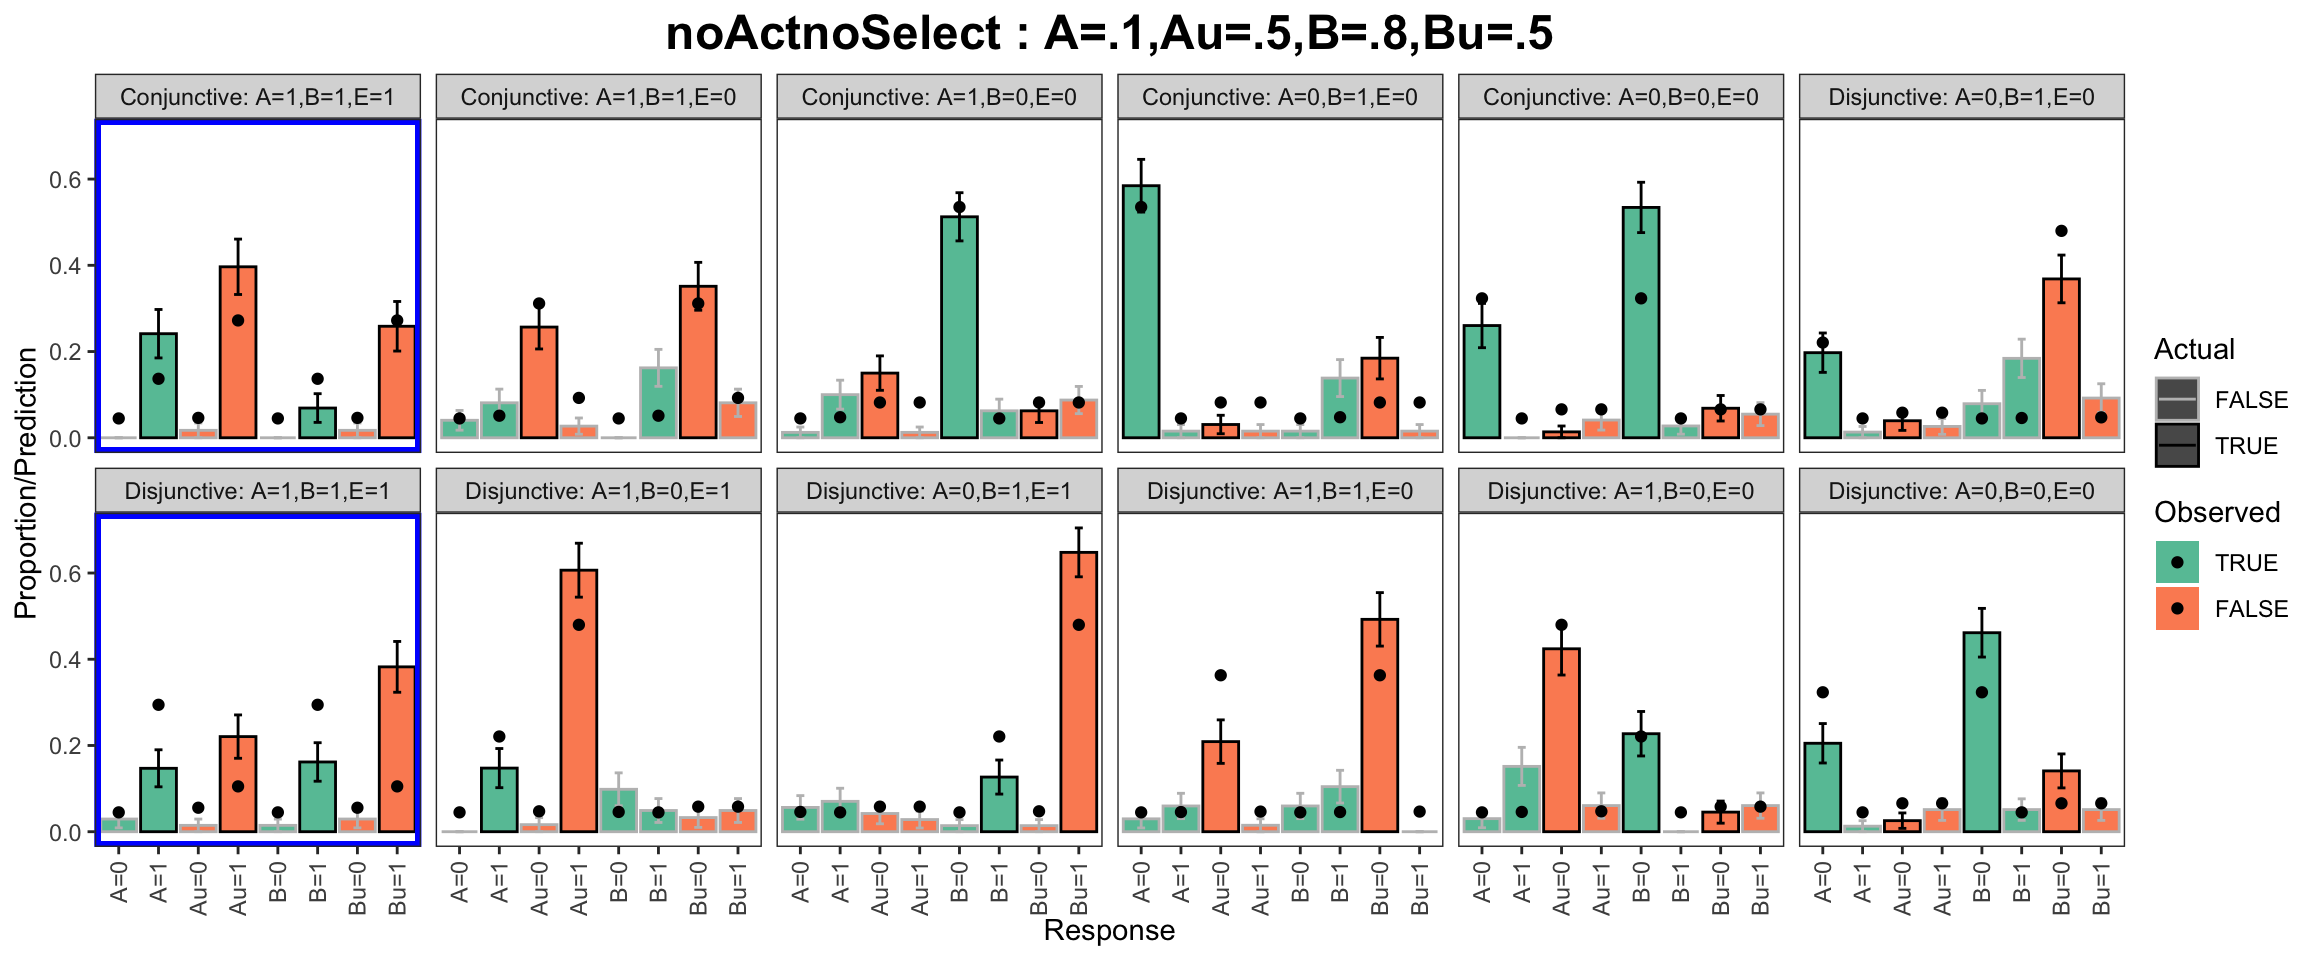
\includegraphics[keepaspectratio]{reportingFigs16m_files/figure-latex/unnamed-chunk-7-16.pdf}}
\pandocbounded{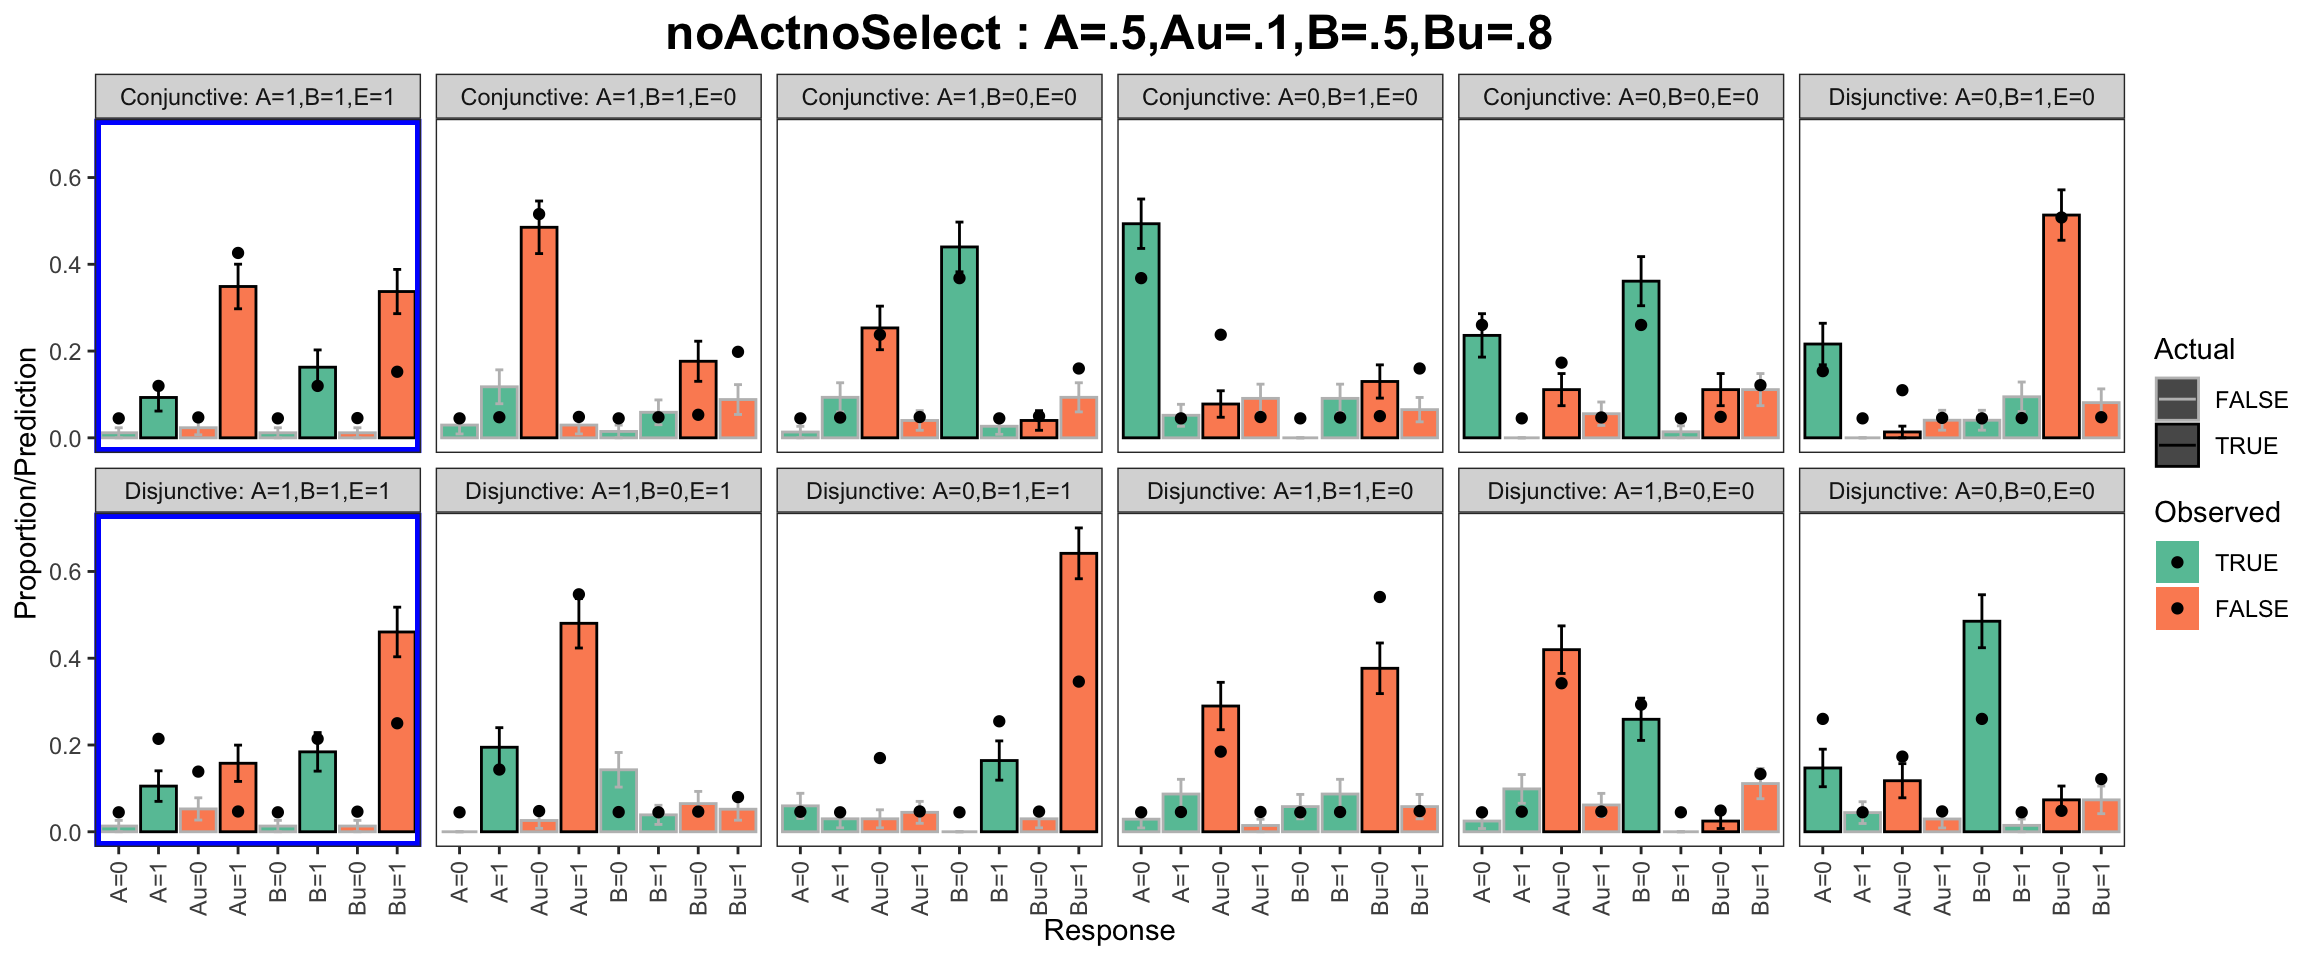
\includegraphics[keepaspectratio]{reportingFigs16m_files/figure-latex/unnamed-chunk-7-17.pdf}}
\pandocbounded{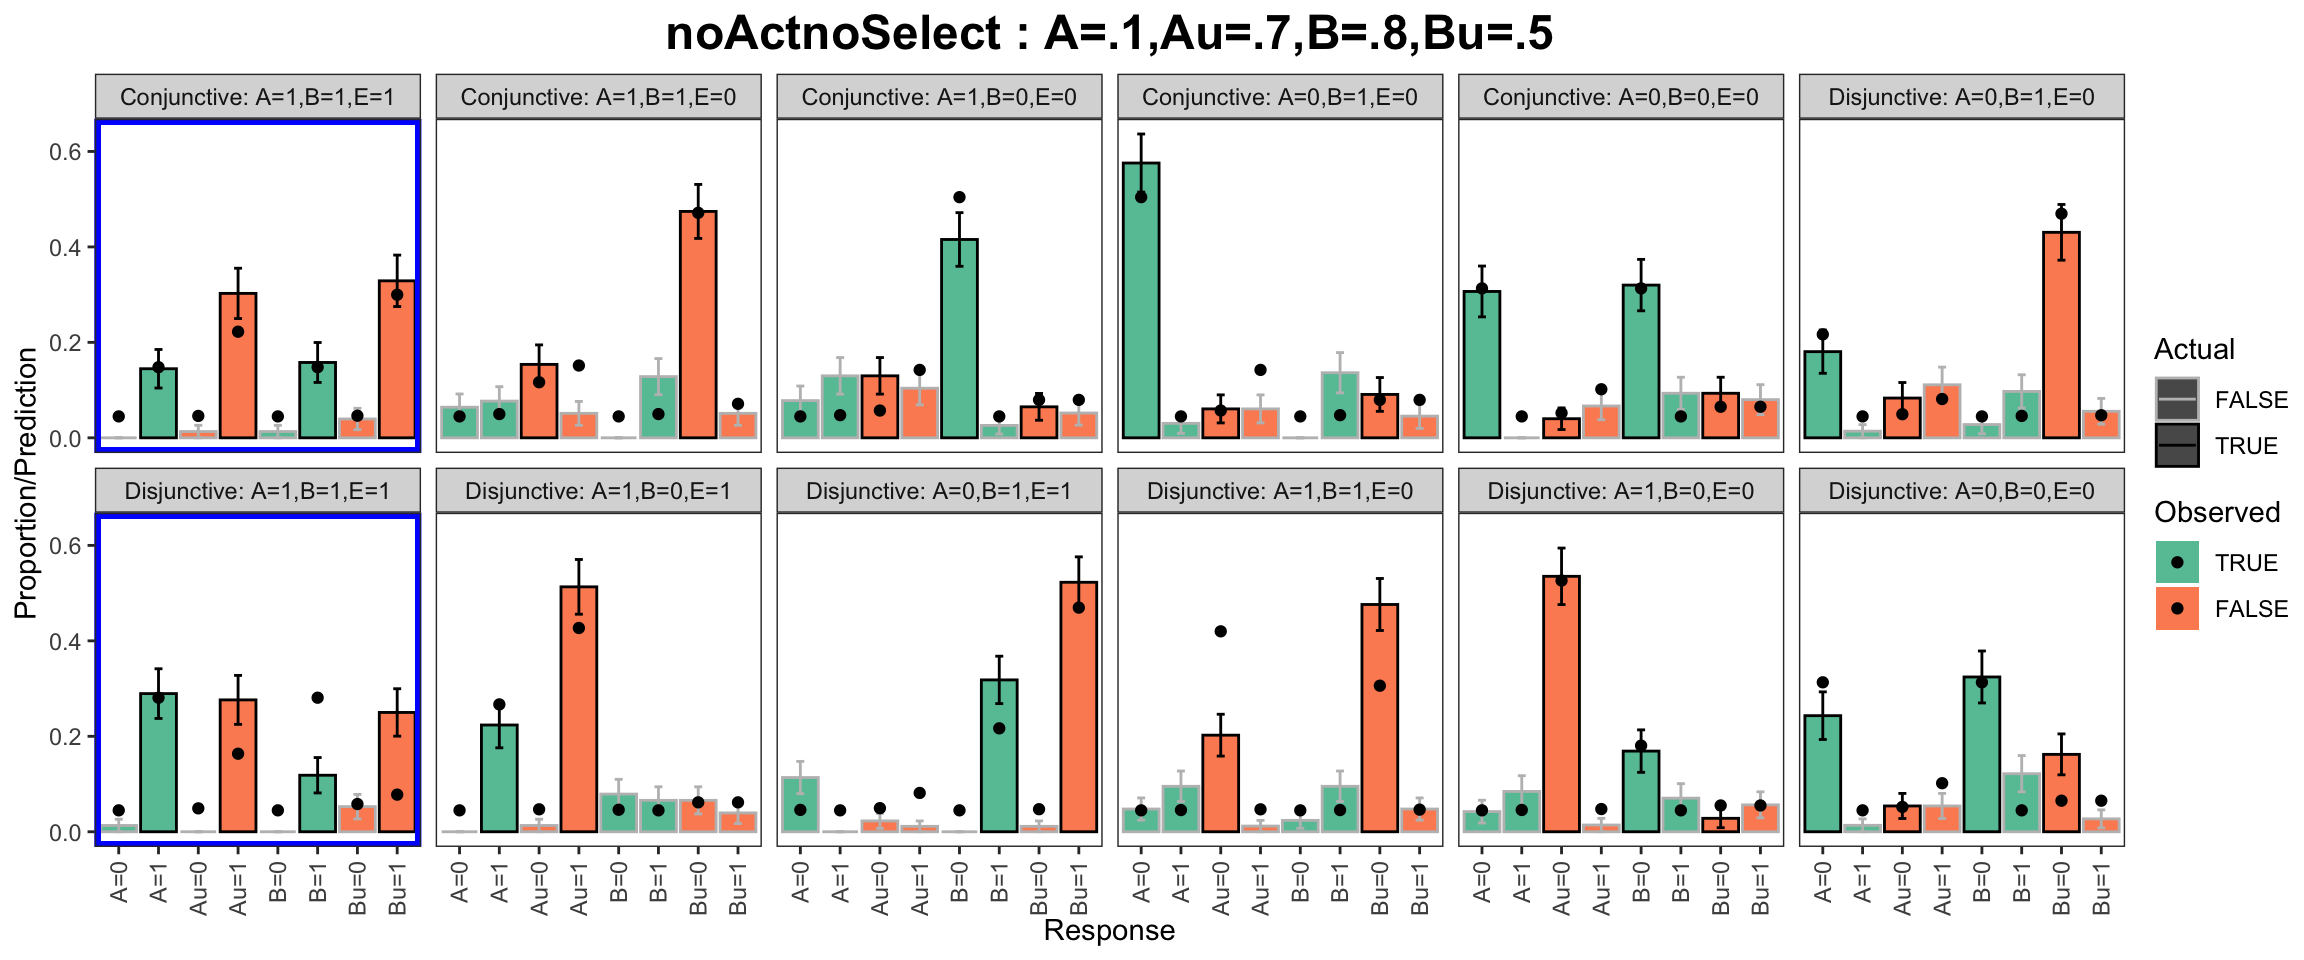
\includegraphics[keepaspectratio]{reportingFigs16m_files/figure-latex/unnamed-chunk-7-18.pdf}}
\pandocbounded{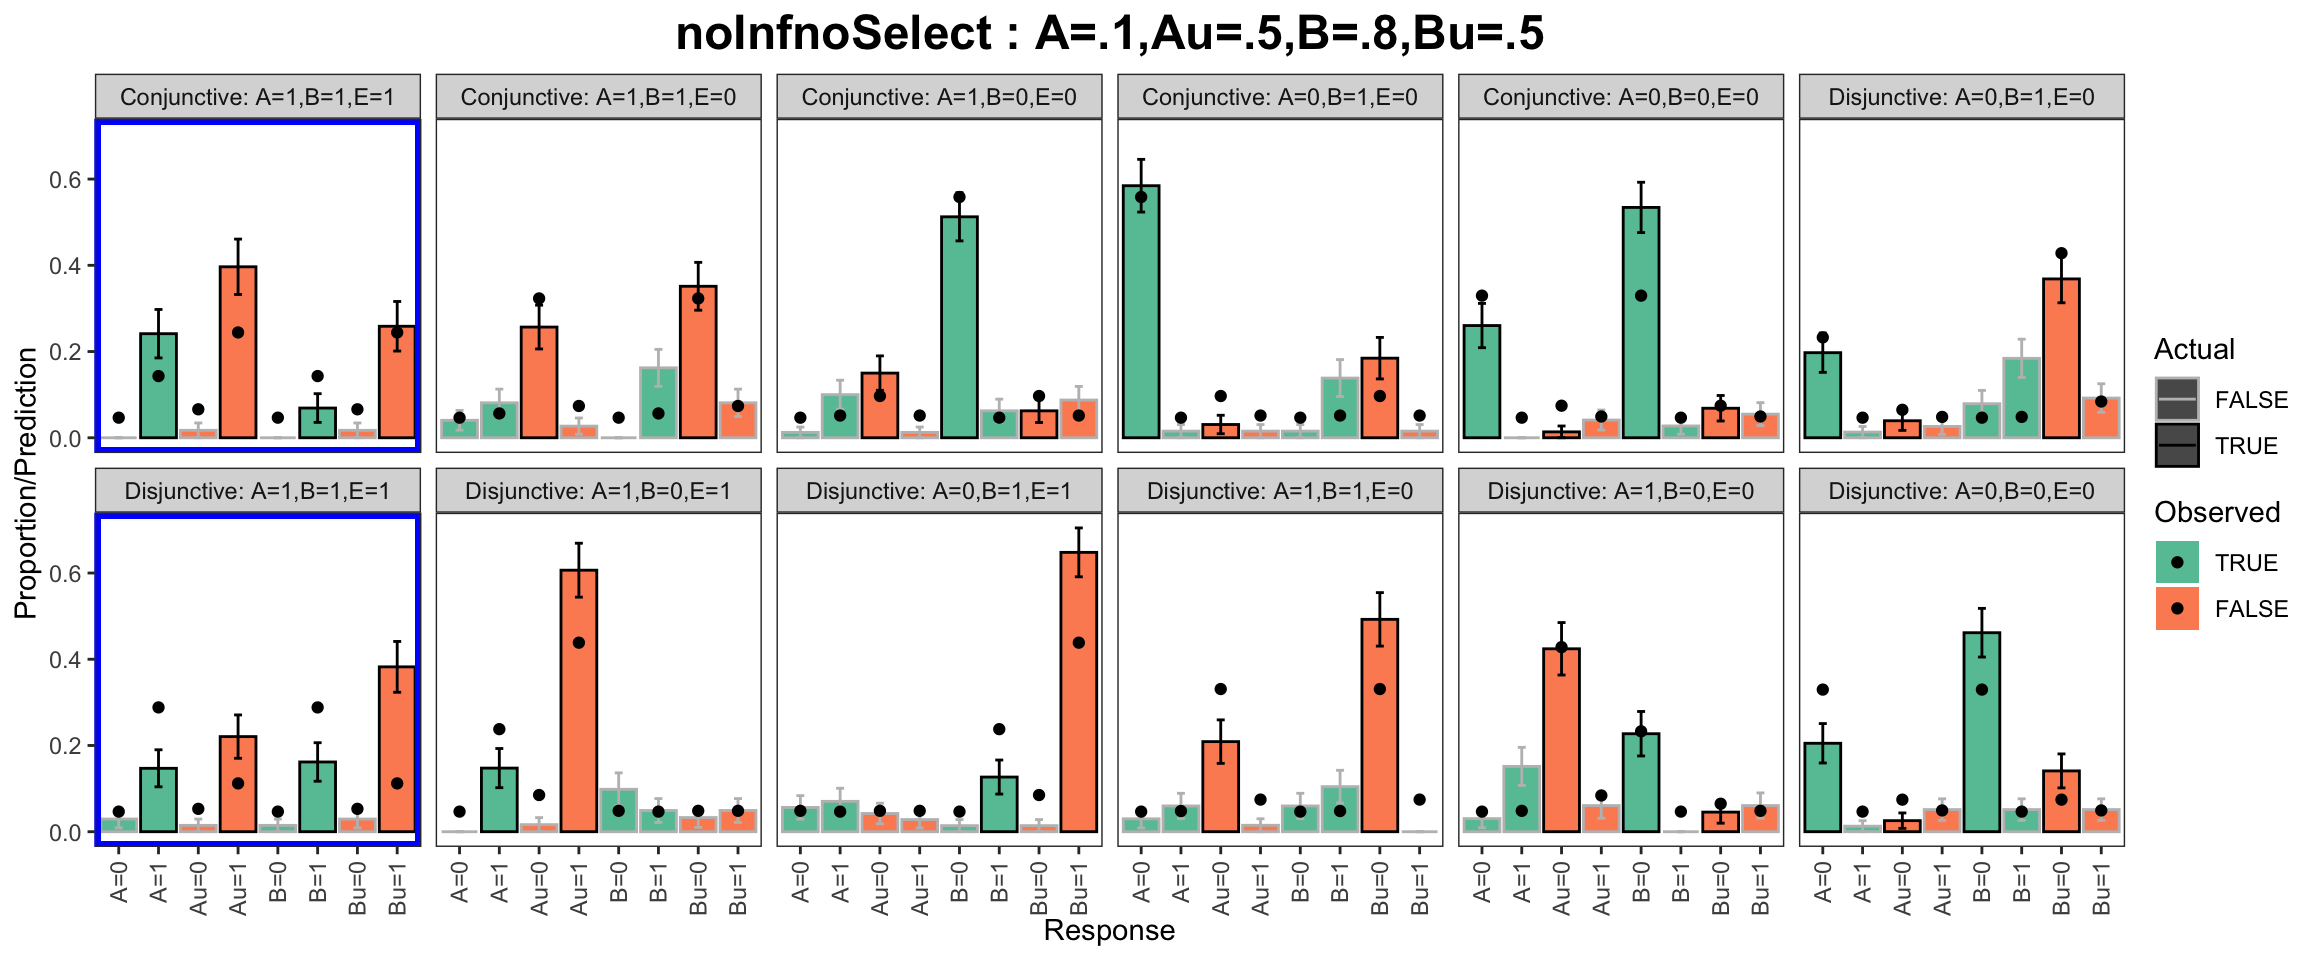
\includegraphics[keepaspectratio]{reportingFigs16m_files/figure-latex/unnamed-chunk-7-19.pdf}}
\pandocbounded{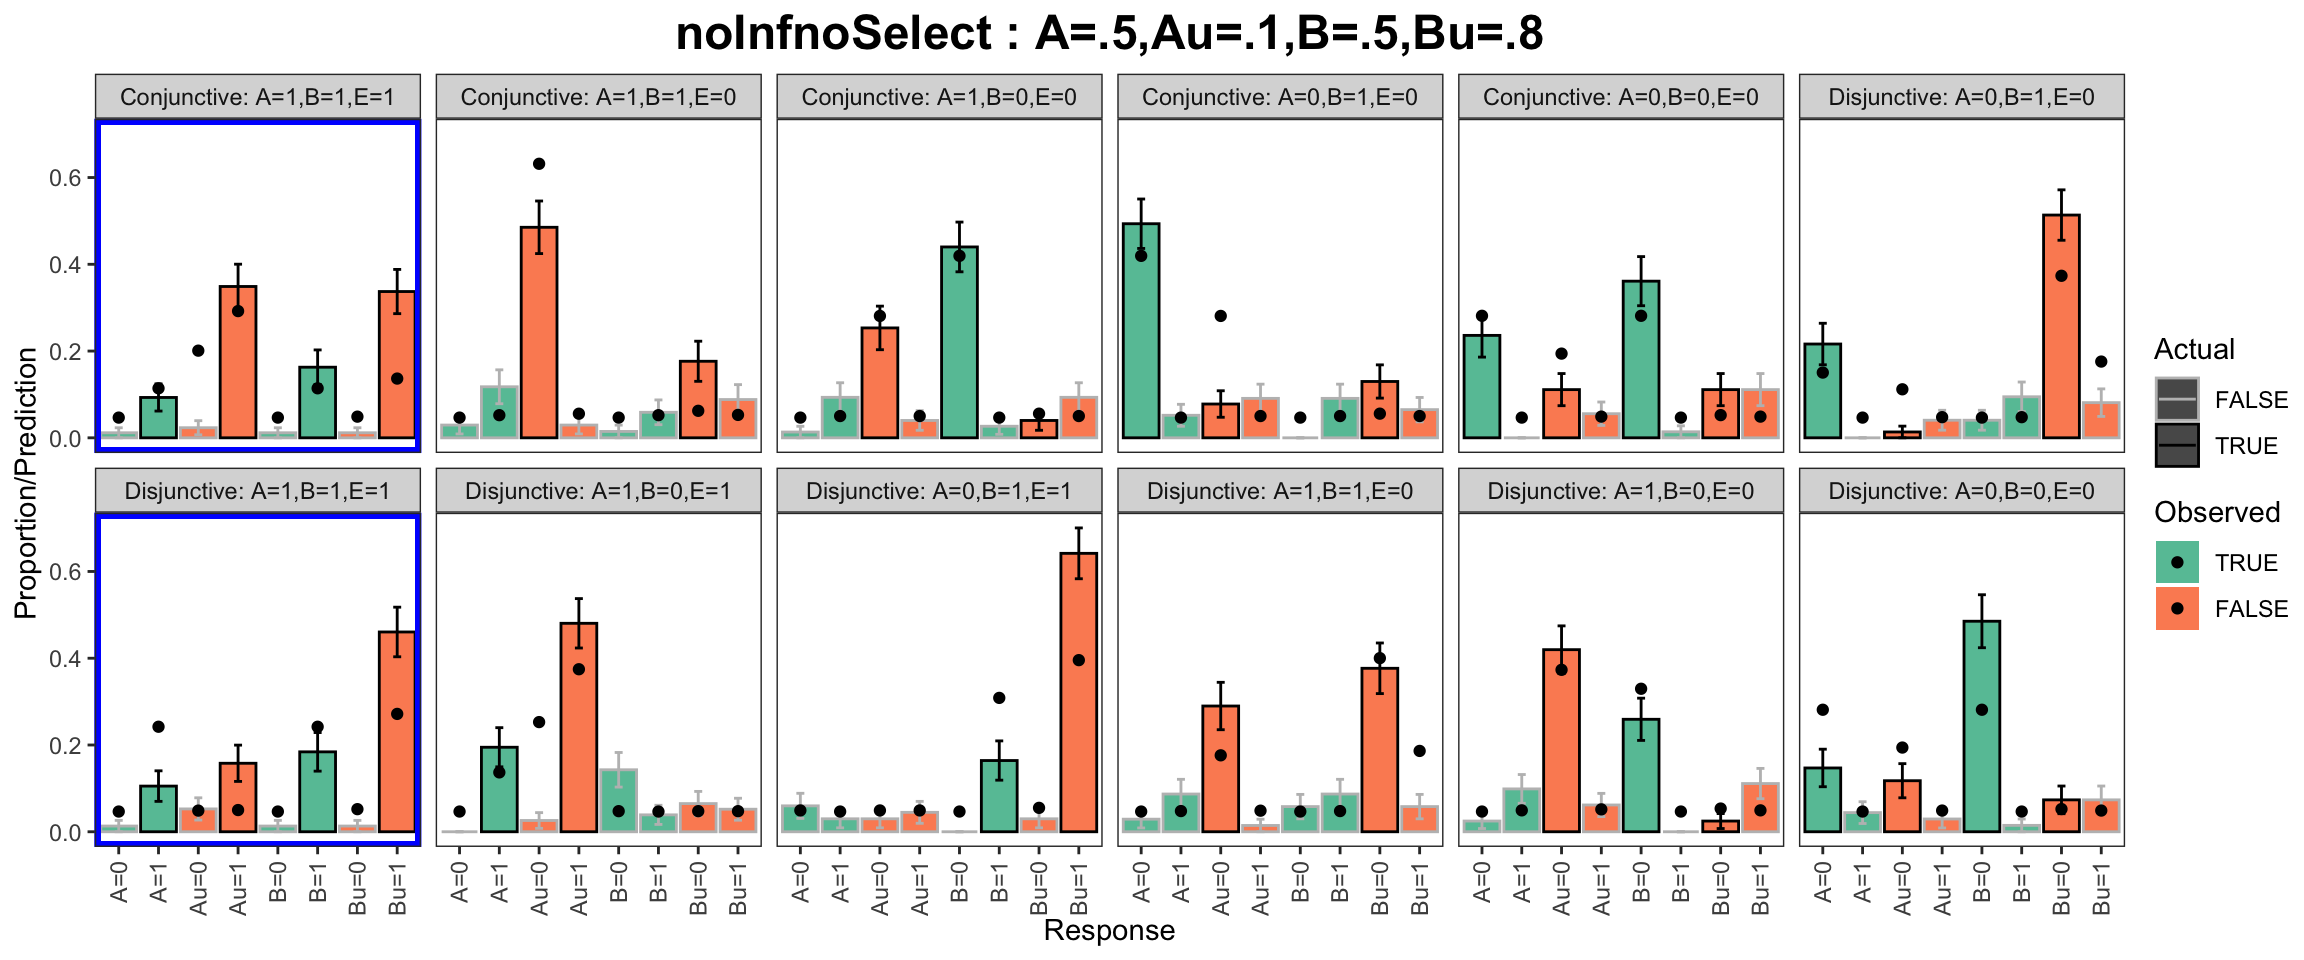
\includegraphics[keepaspectratio]{reportingFigs16m_files/figure-latex/unnamed-chunk-7-20.pdf}}
\pandocbounded{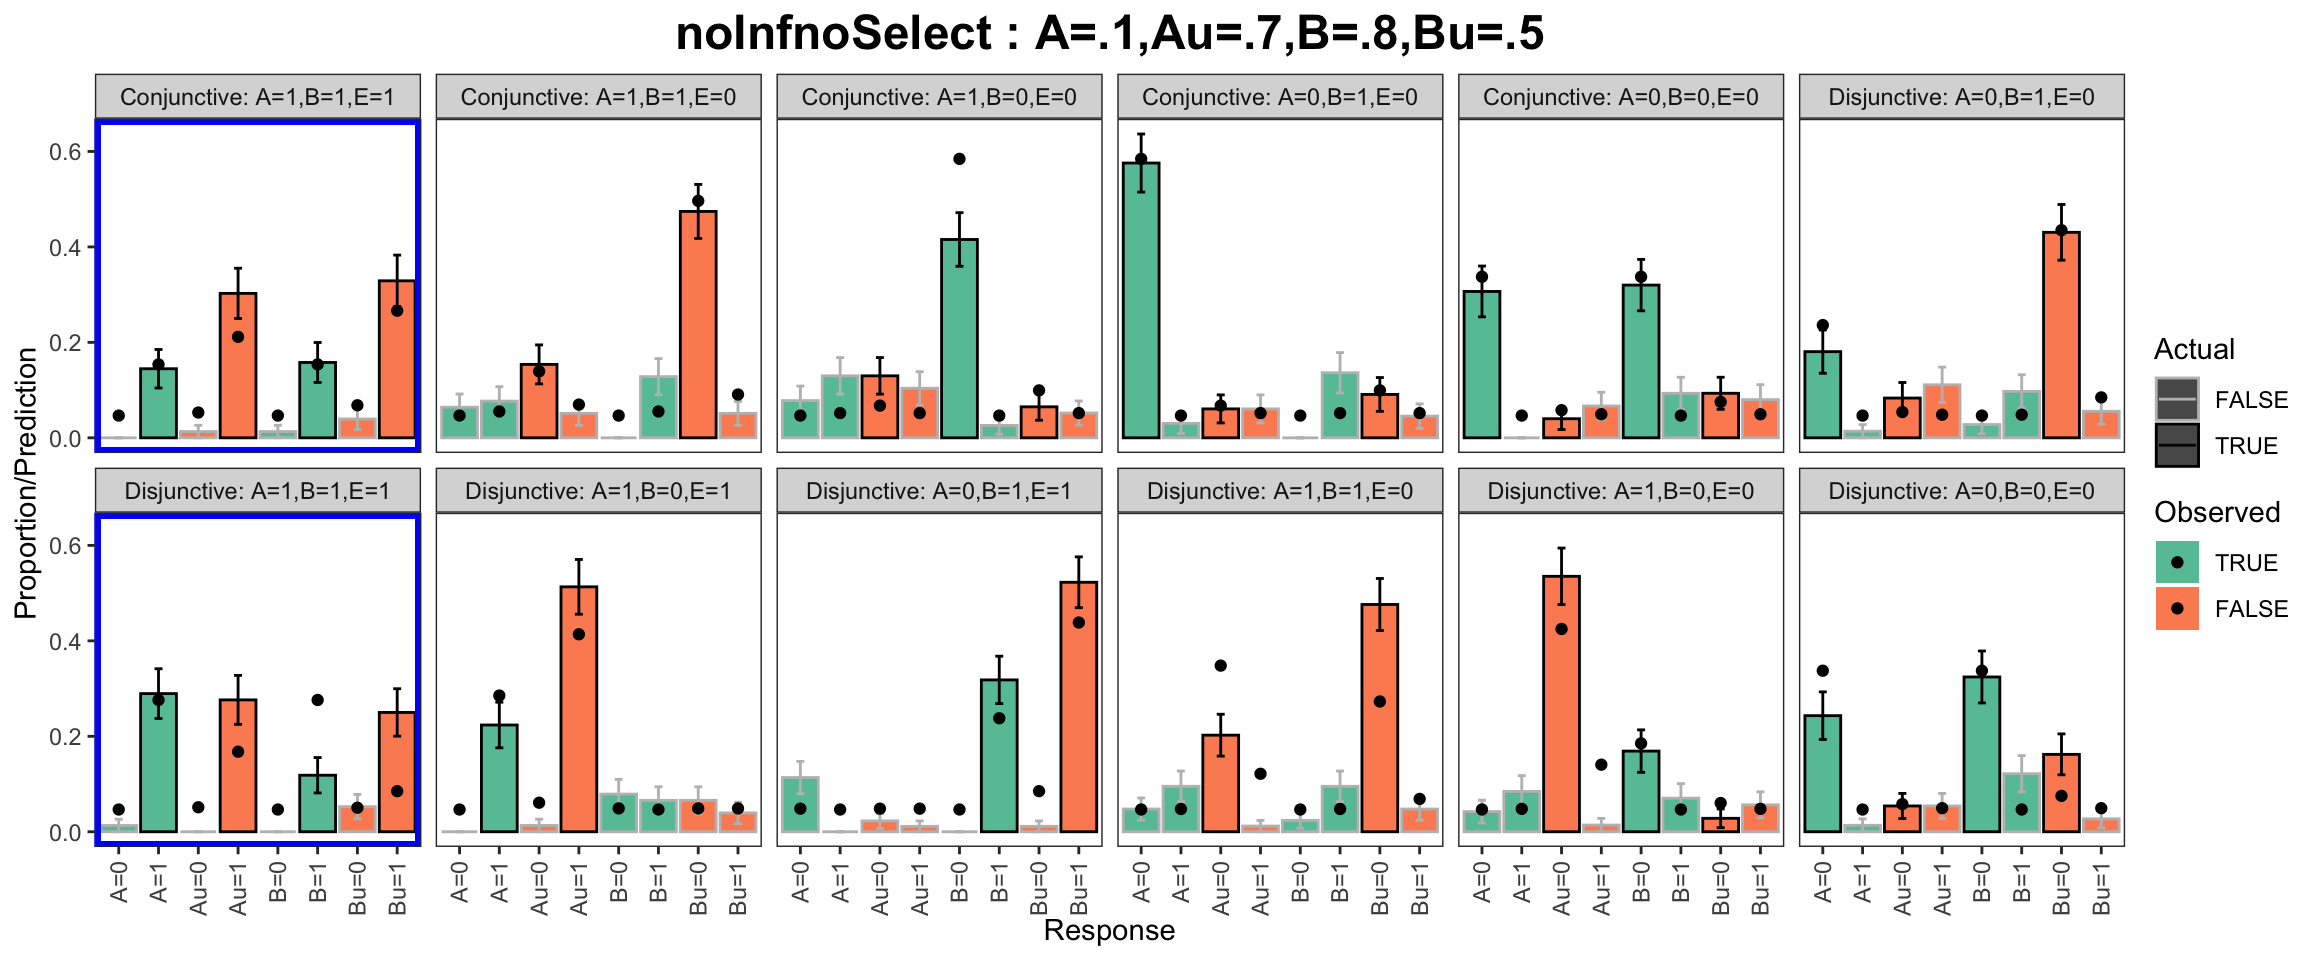
\includegraphics[keepaspectratio]{reportingFigs16m_files/figure-latex/unnamed-chunk-7-21.pdf}}
\pandocbounded{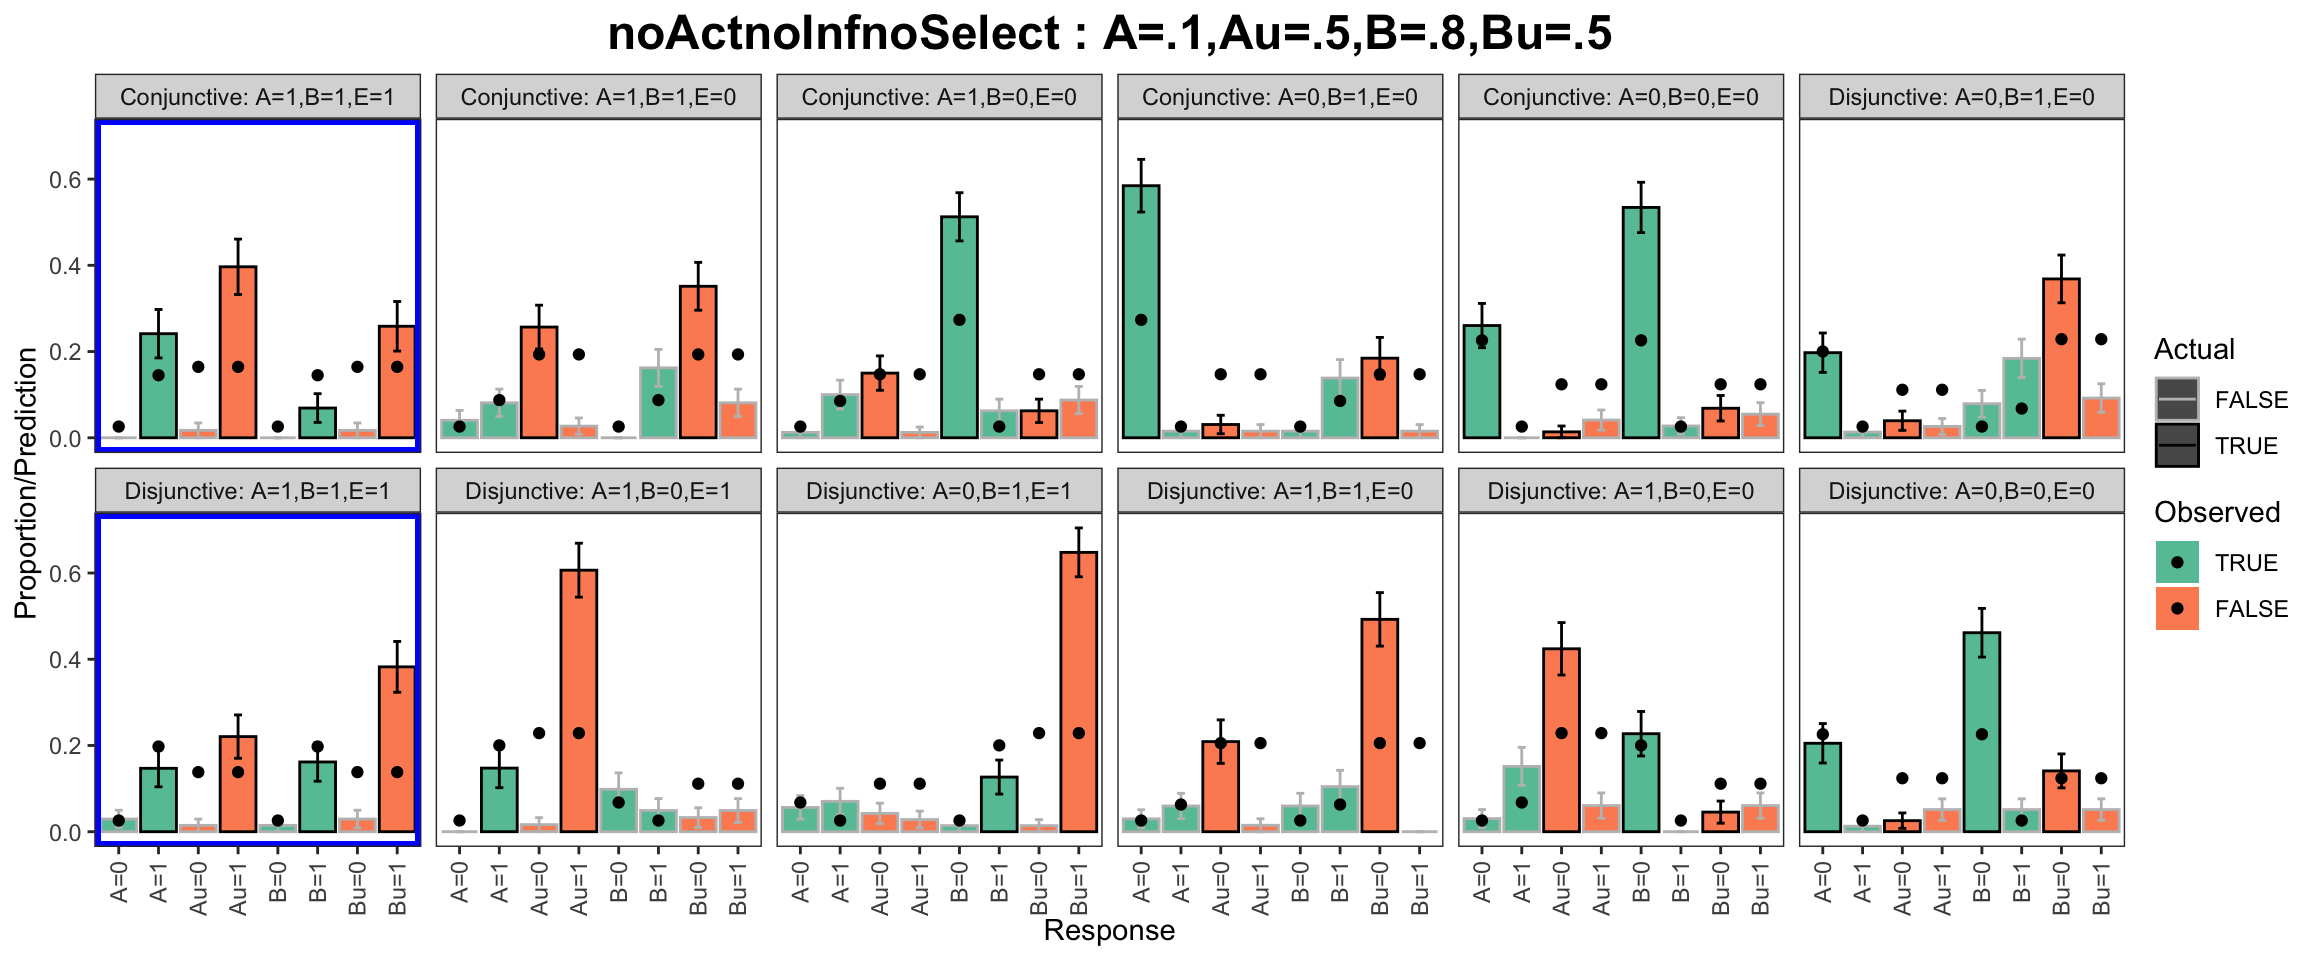
\includegraphics[keepaspectratio]{reportingFigs16m_files/figure-latex/unnamed-chunk-7-22.pdf}}
\pandocbounded{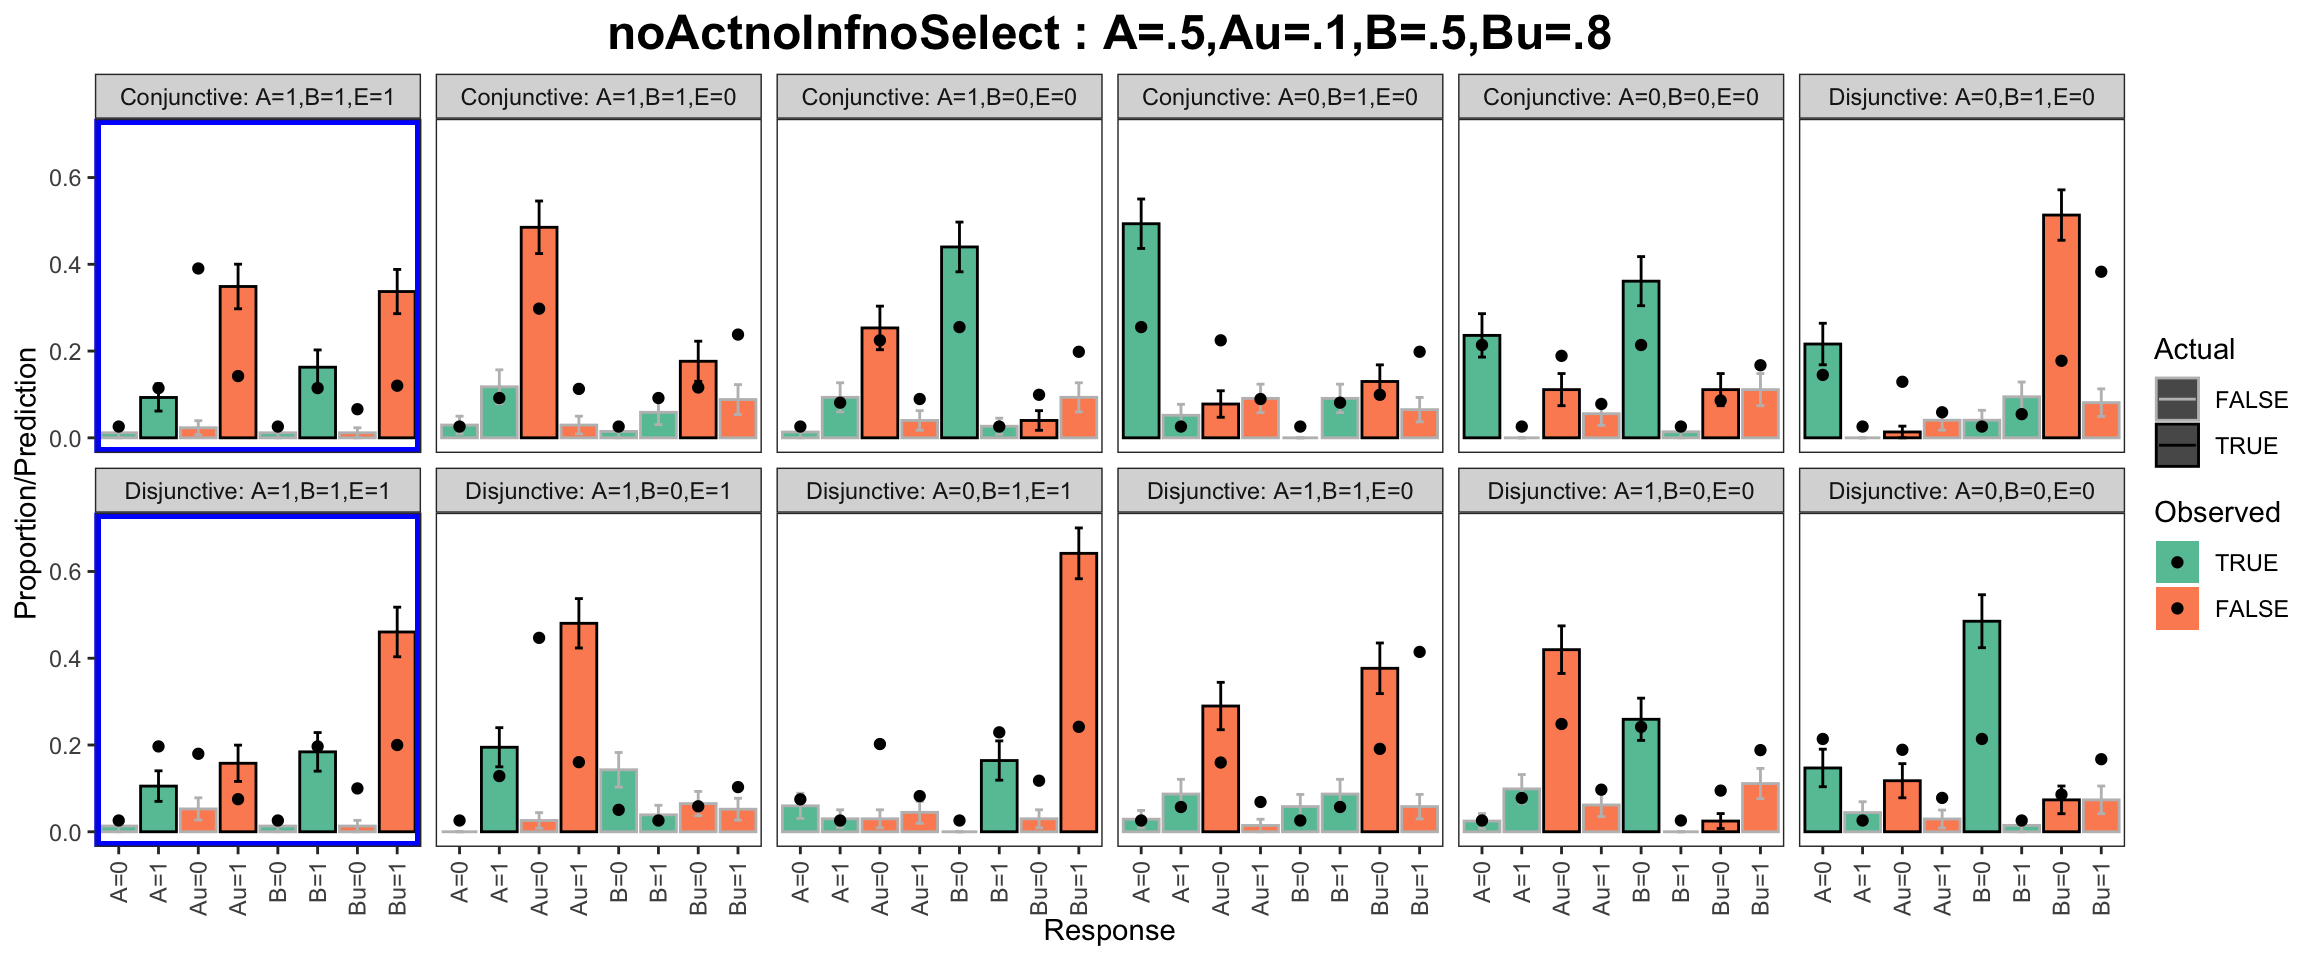
\includegraphics[keepaspectratio]{reportingFigs16m_files/figure-latex/unnamed-chunk-7-23.pdf}}
\pandocbounded{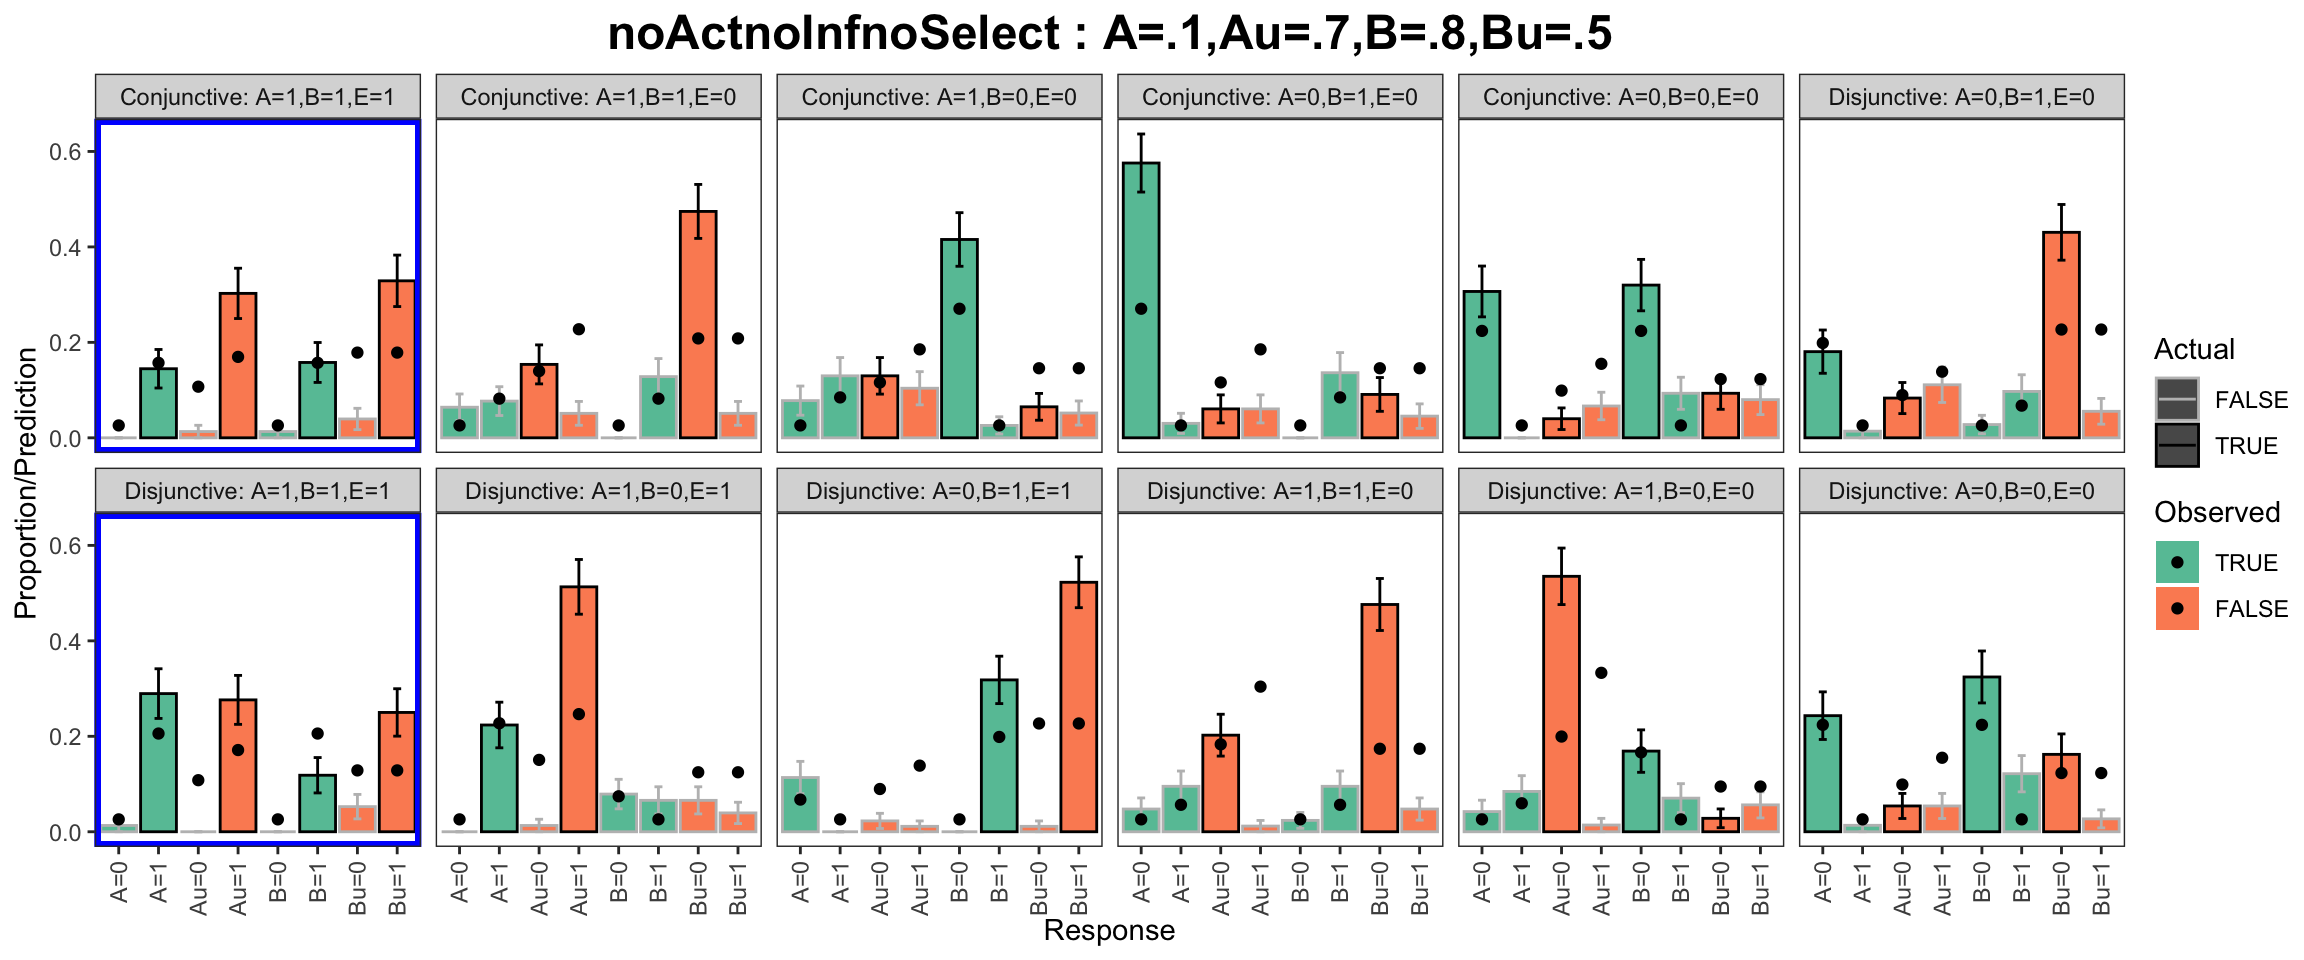
\includegraphics[keepaspectratio]{reportingFigs16m_files/figure-latex/unnamed-chunk-7-24.pdf}}
\pandocbounded{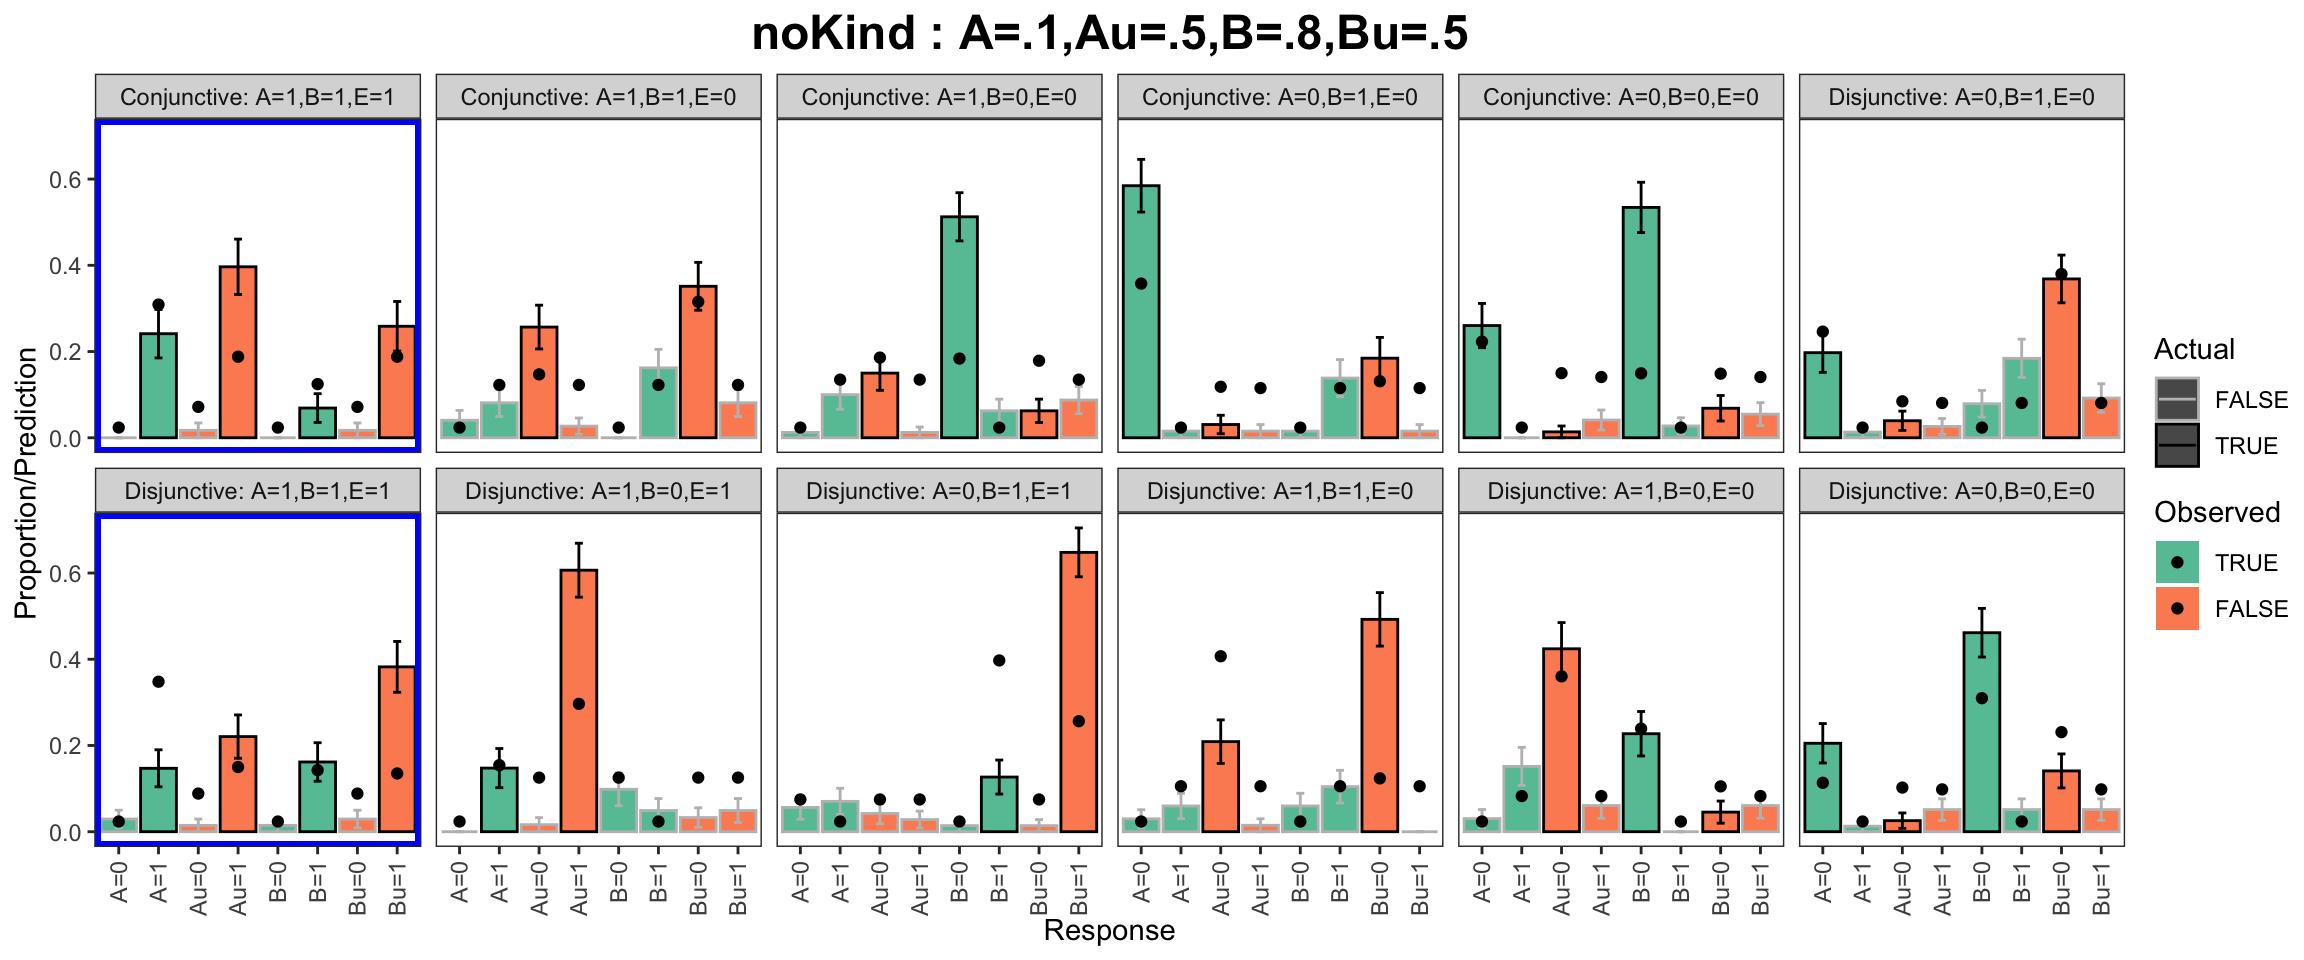
\includegraphics[keepaspectratio]{reportingFigs16m_files/figure-latex/unnamed-chunk-7-25.pdf}}
\pandocbounded{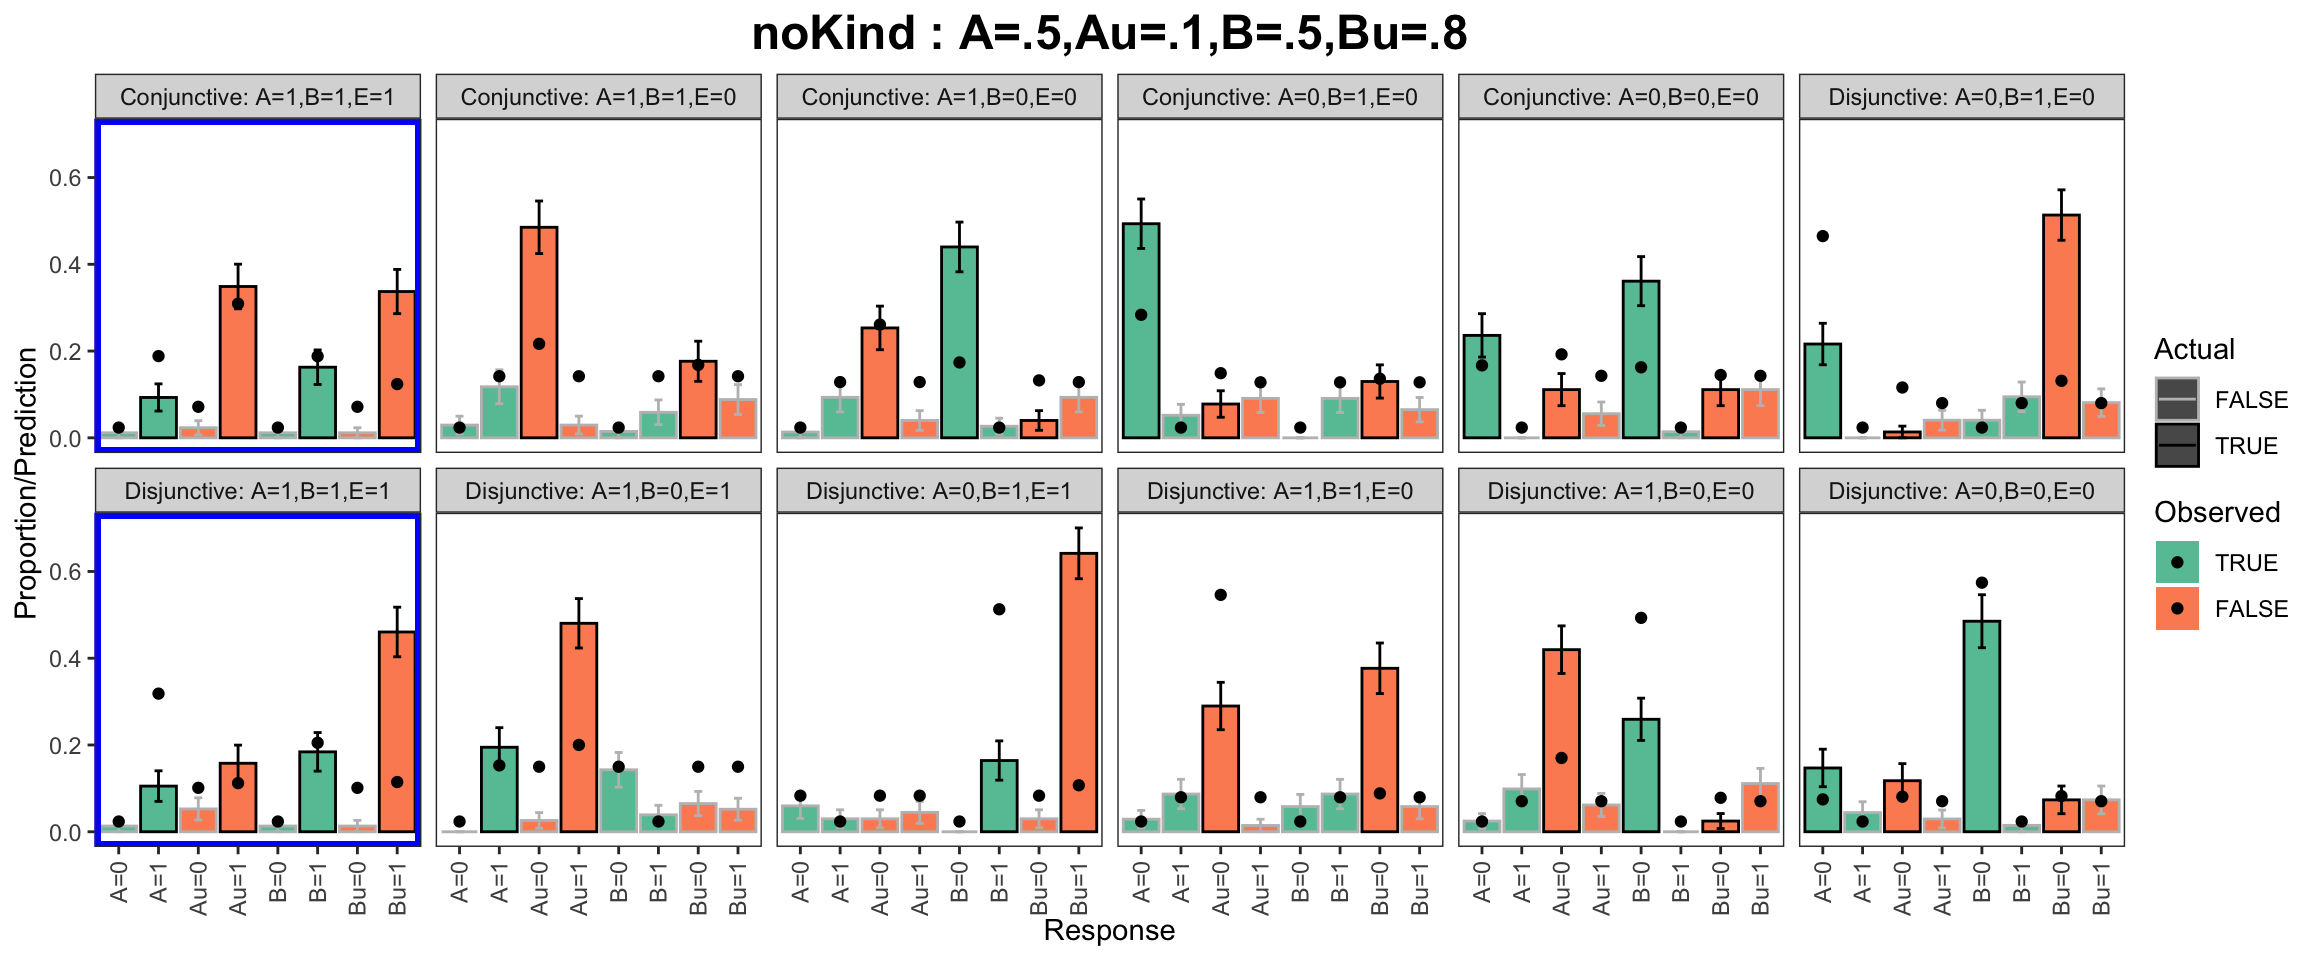
\includegraphics[keepaspectratio]{reportingFigs16m_files/figure-latex/unnamed-chunk-7-26.pdf}}
\pandocbounded{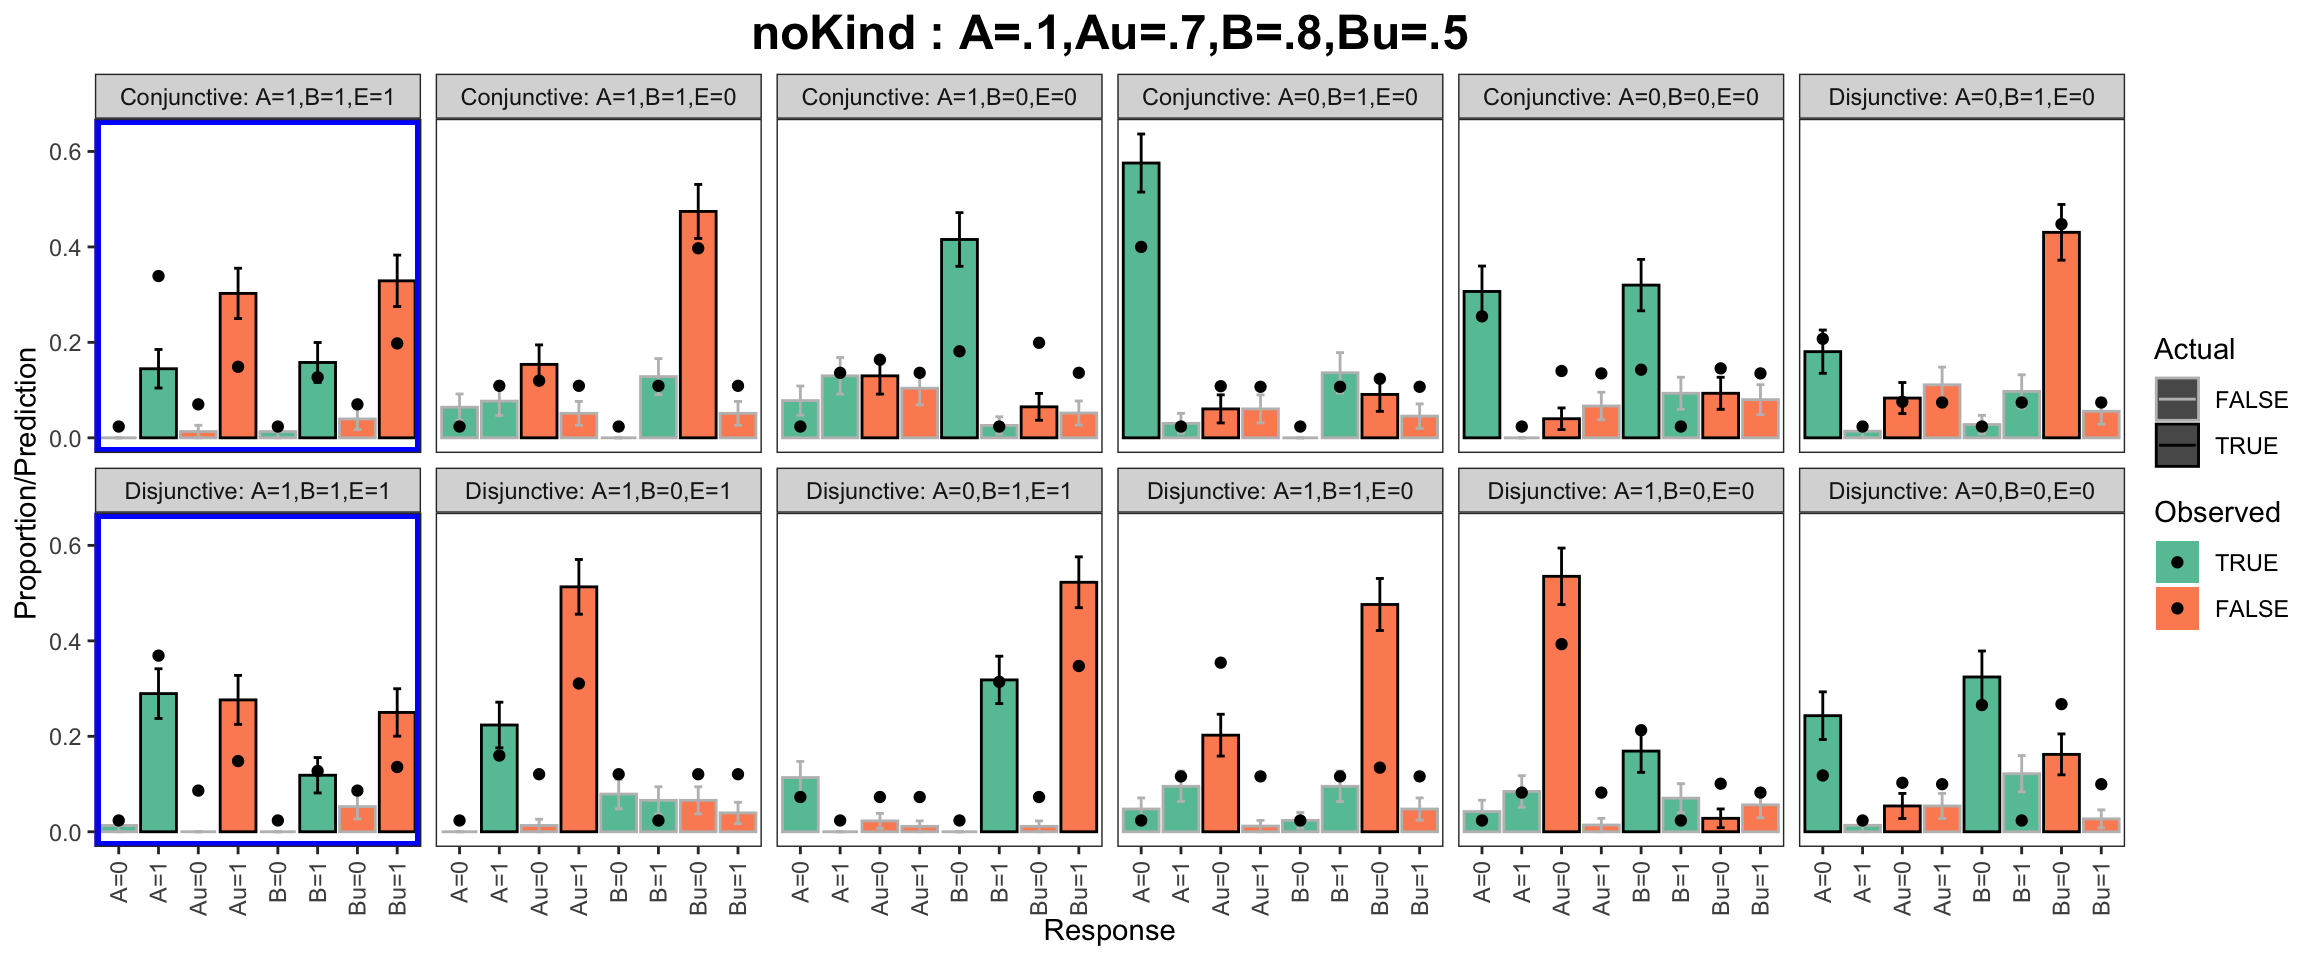
\includegraphics[keepaspectratio]{reportingFigs16m_files/figure-latex/unnamed-chunk-7-27.pdf}}
\pandocbounded{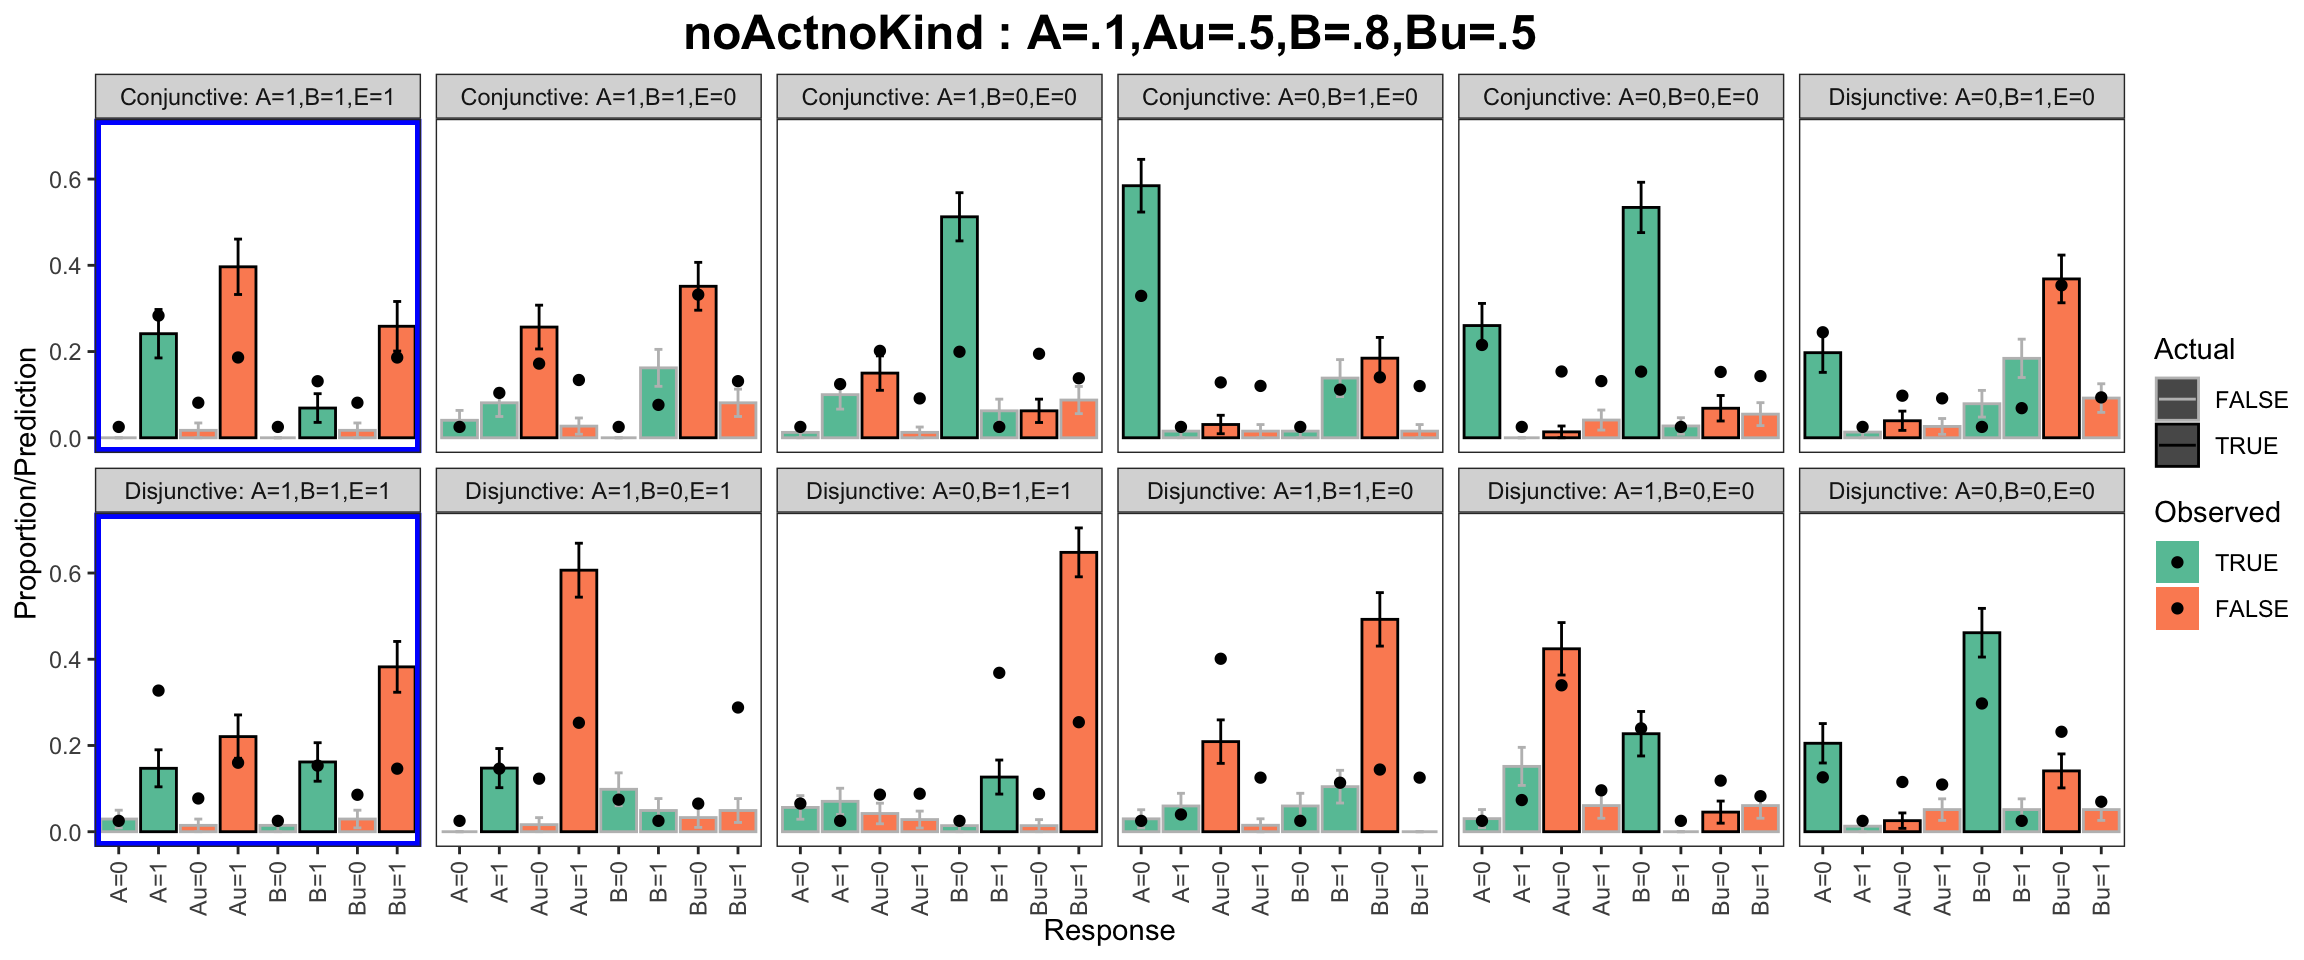
\includegraphics[keepaspectratio]{reportingFigs16m_files/figure-latex/unnamed-chunk-7-28.pdf}}
\pandocbounded{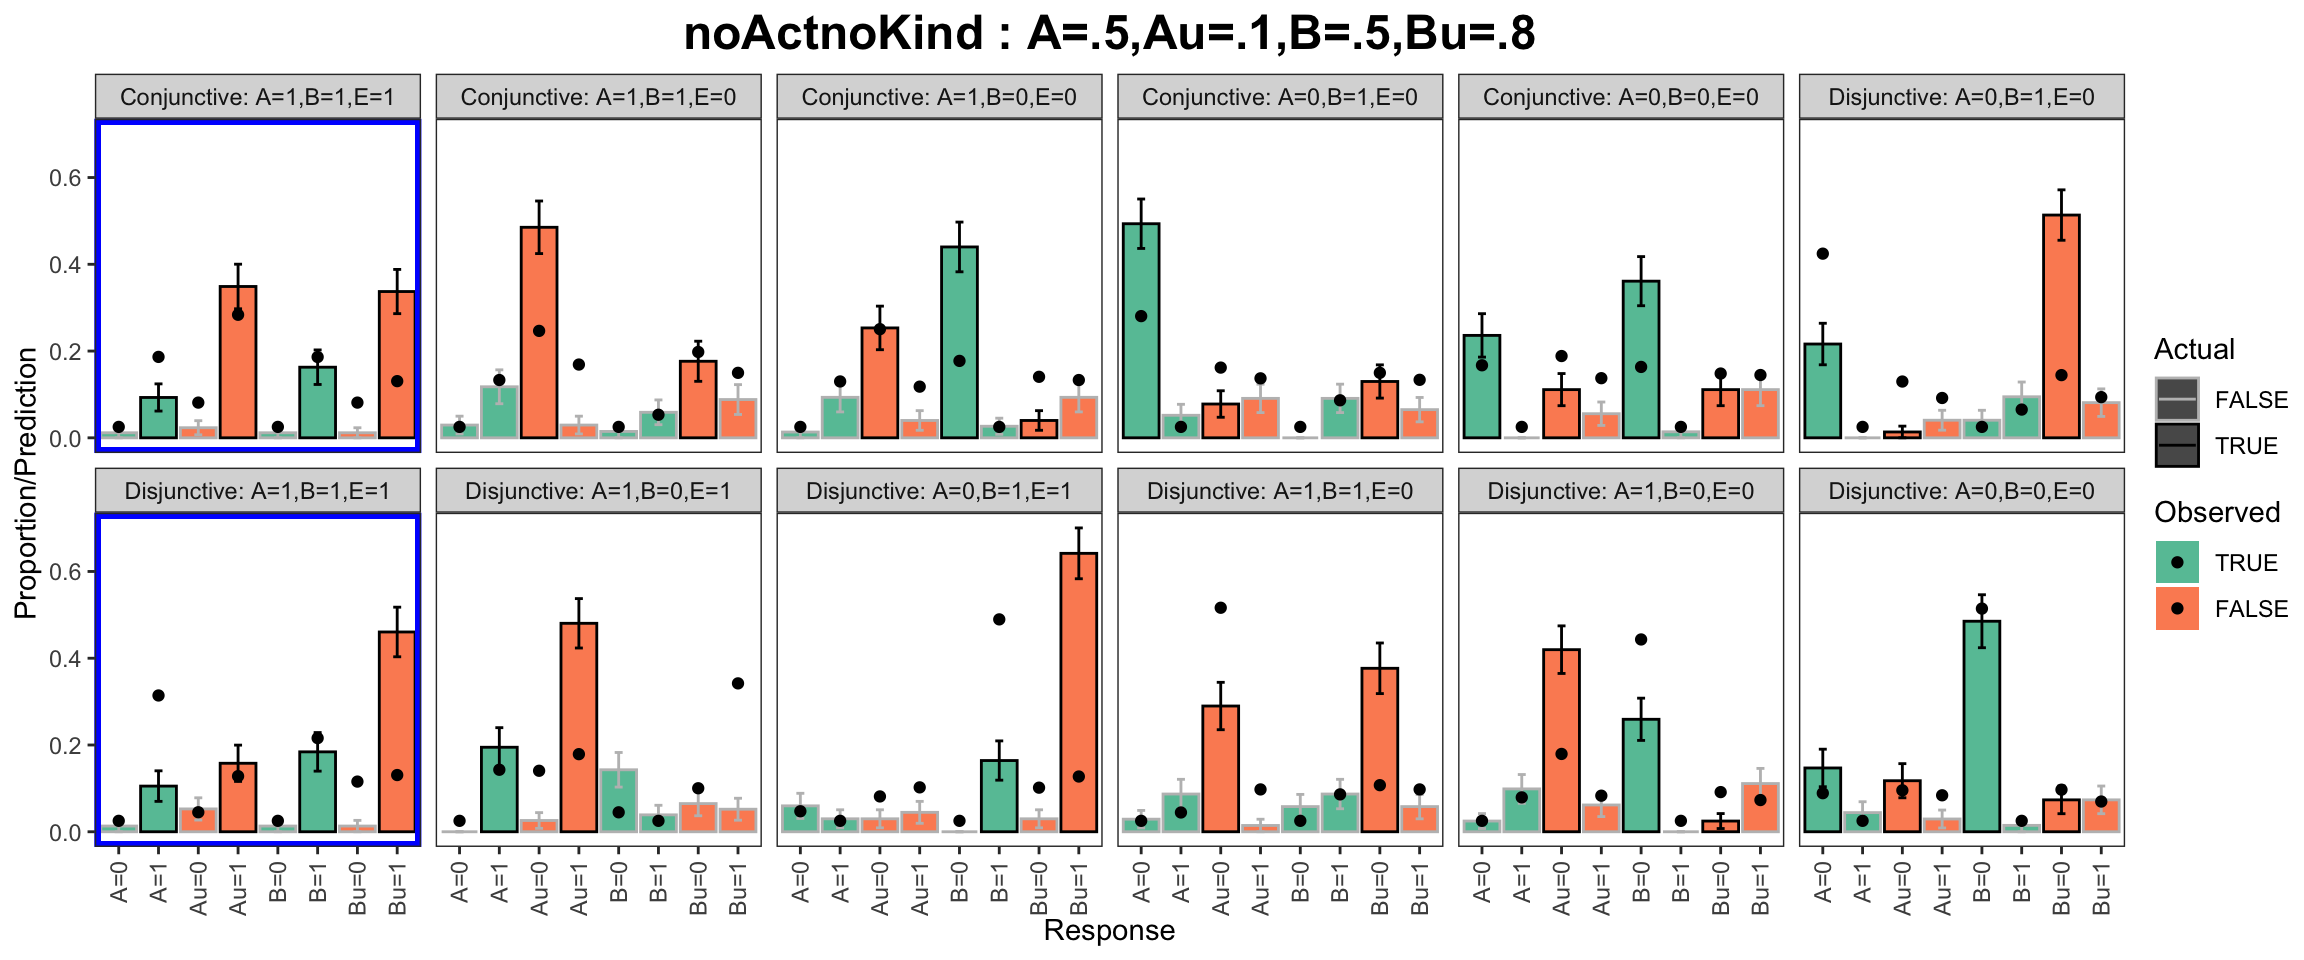
\includegraphics[keepaspectratio]{reportingFigs16m_files/figure-latex/unnamed-chunk-7-29.pdf}}
\pandocbounded{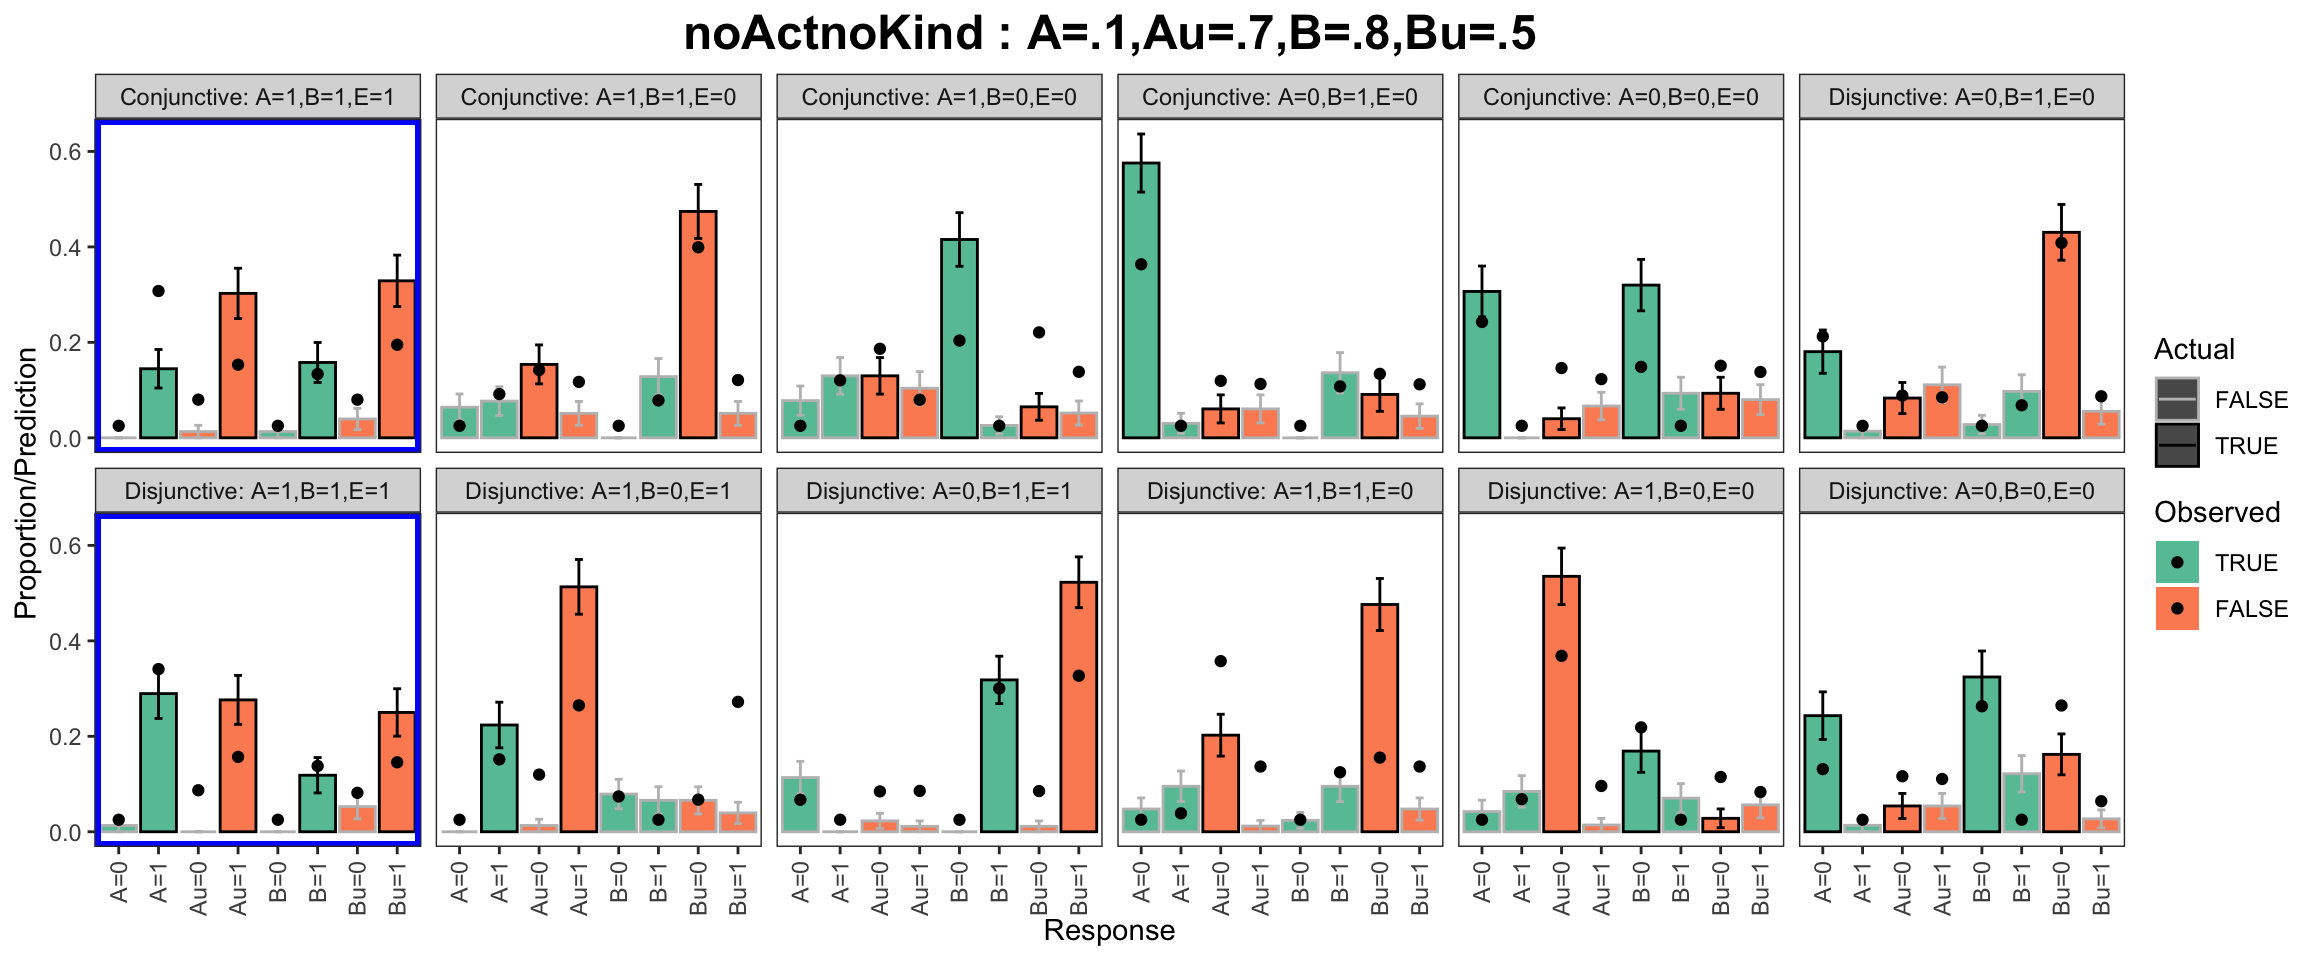
\includegraphics[keepaspectratio]{reportingFigs16m_files/figure-latex/unnamed-chunk-7-30.pdf}}
\pandocbounded{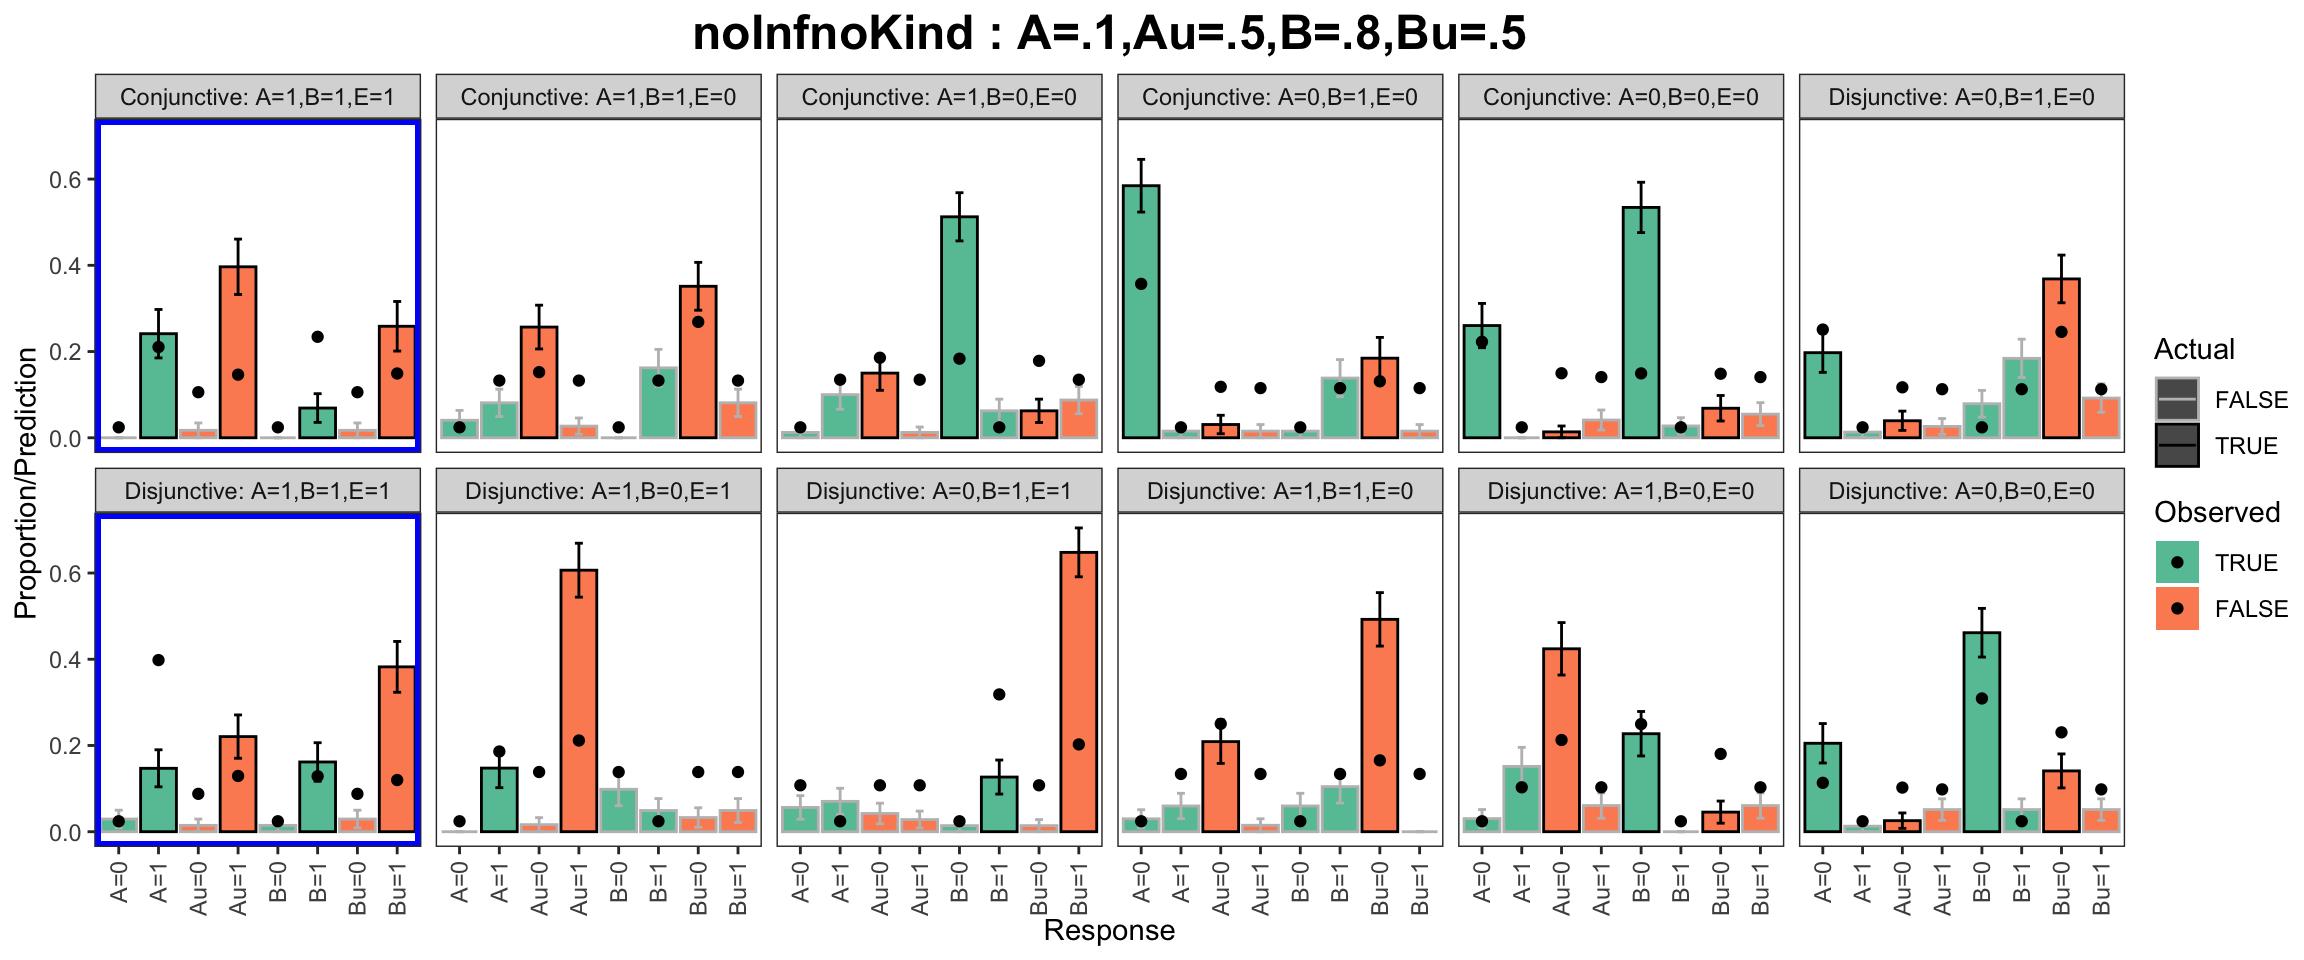
\includegraphics[keepaspectratio]{reportingFigs16m_files/figure-latex/unnamed-chunk-7-31.pdf}}
\pandocbounded{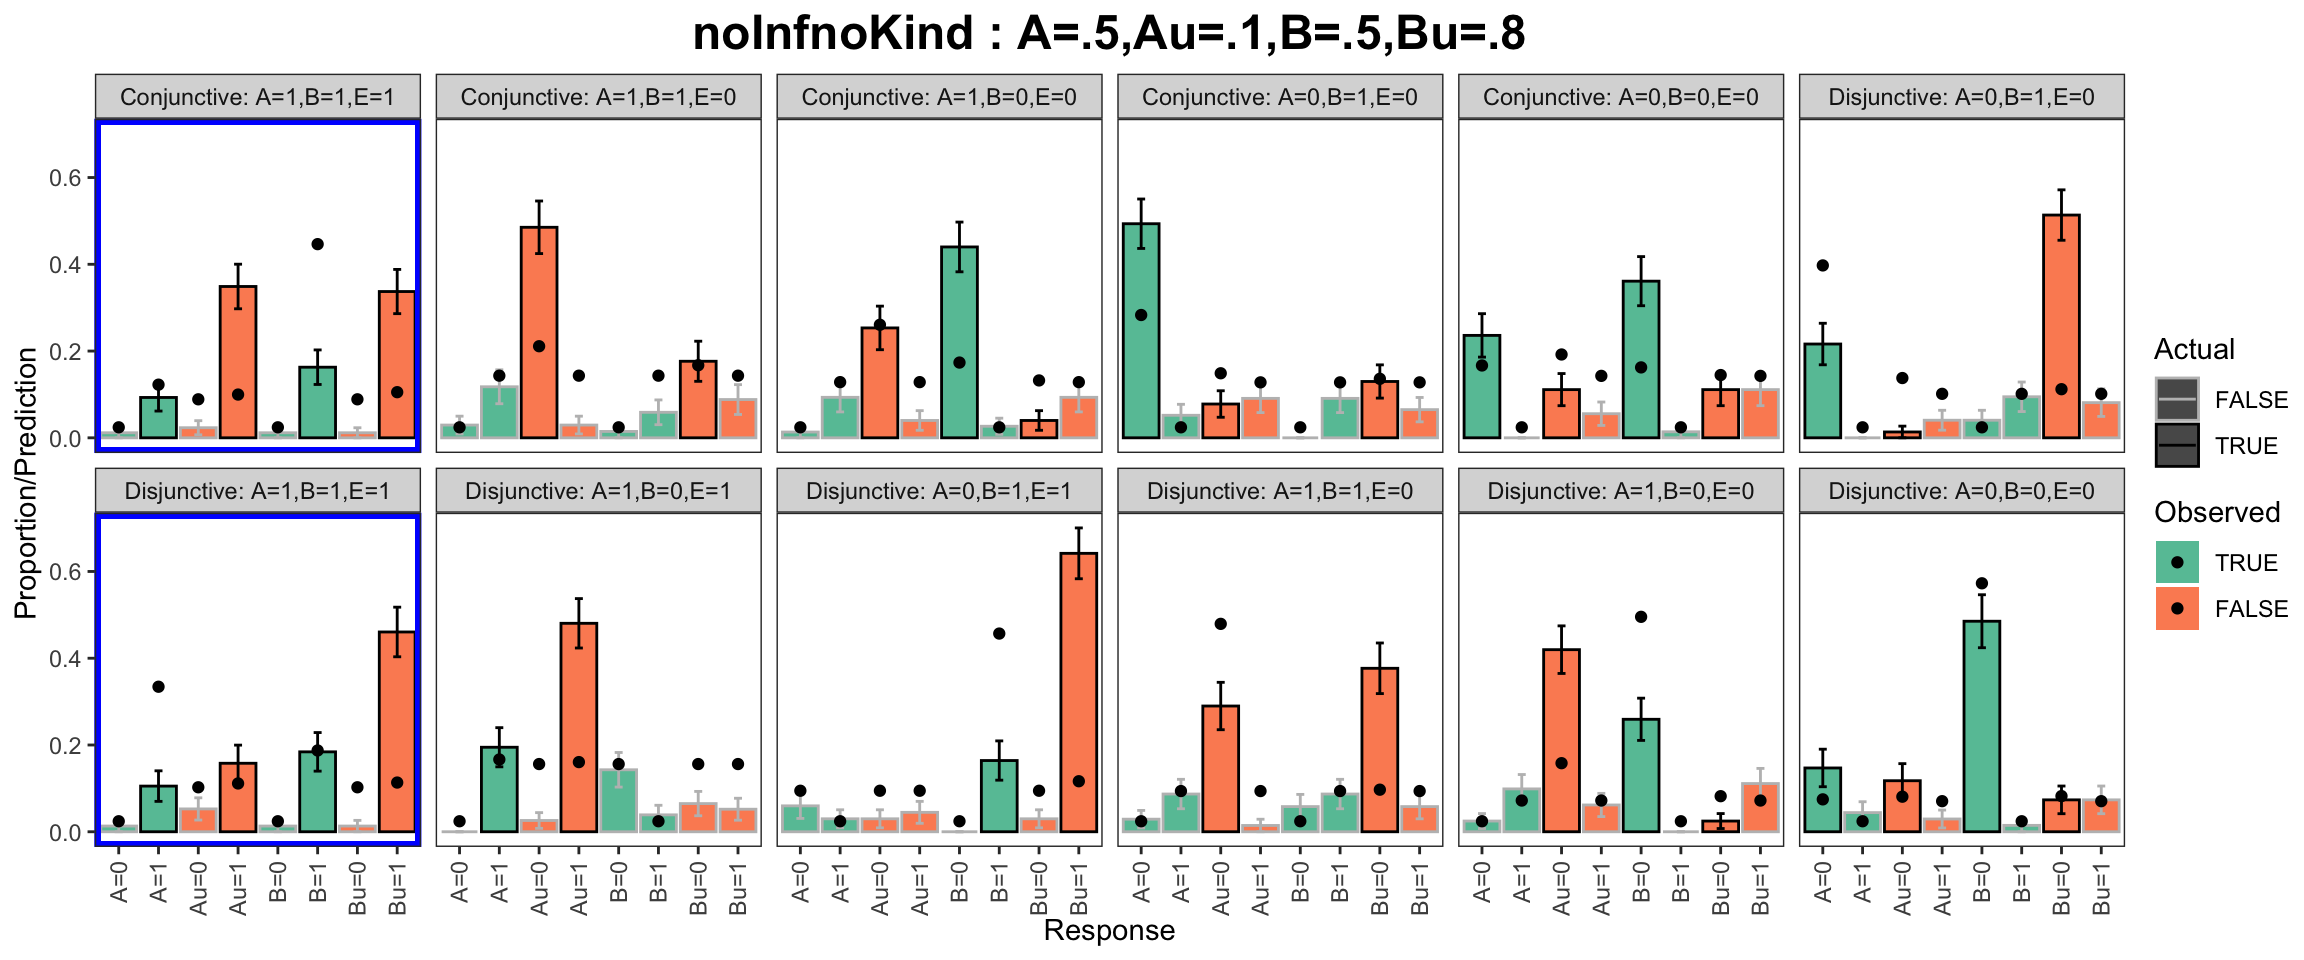
\includegraphics[keepaspectratio]{reportingFigs16m_files/figure-latex/unnamed-chunk-7-32.pdf}}
\pandocbounded{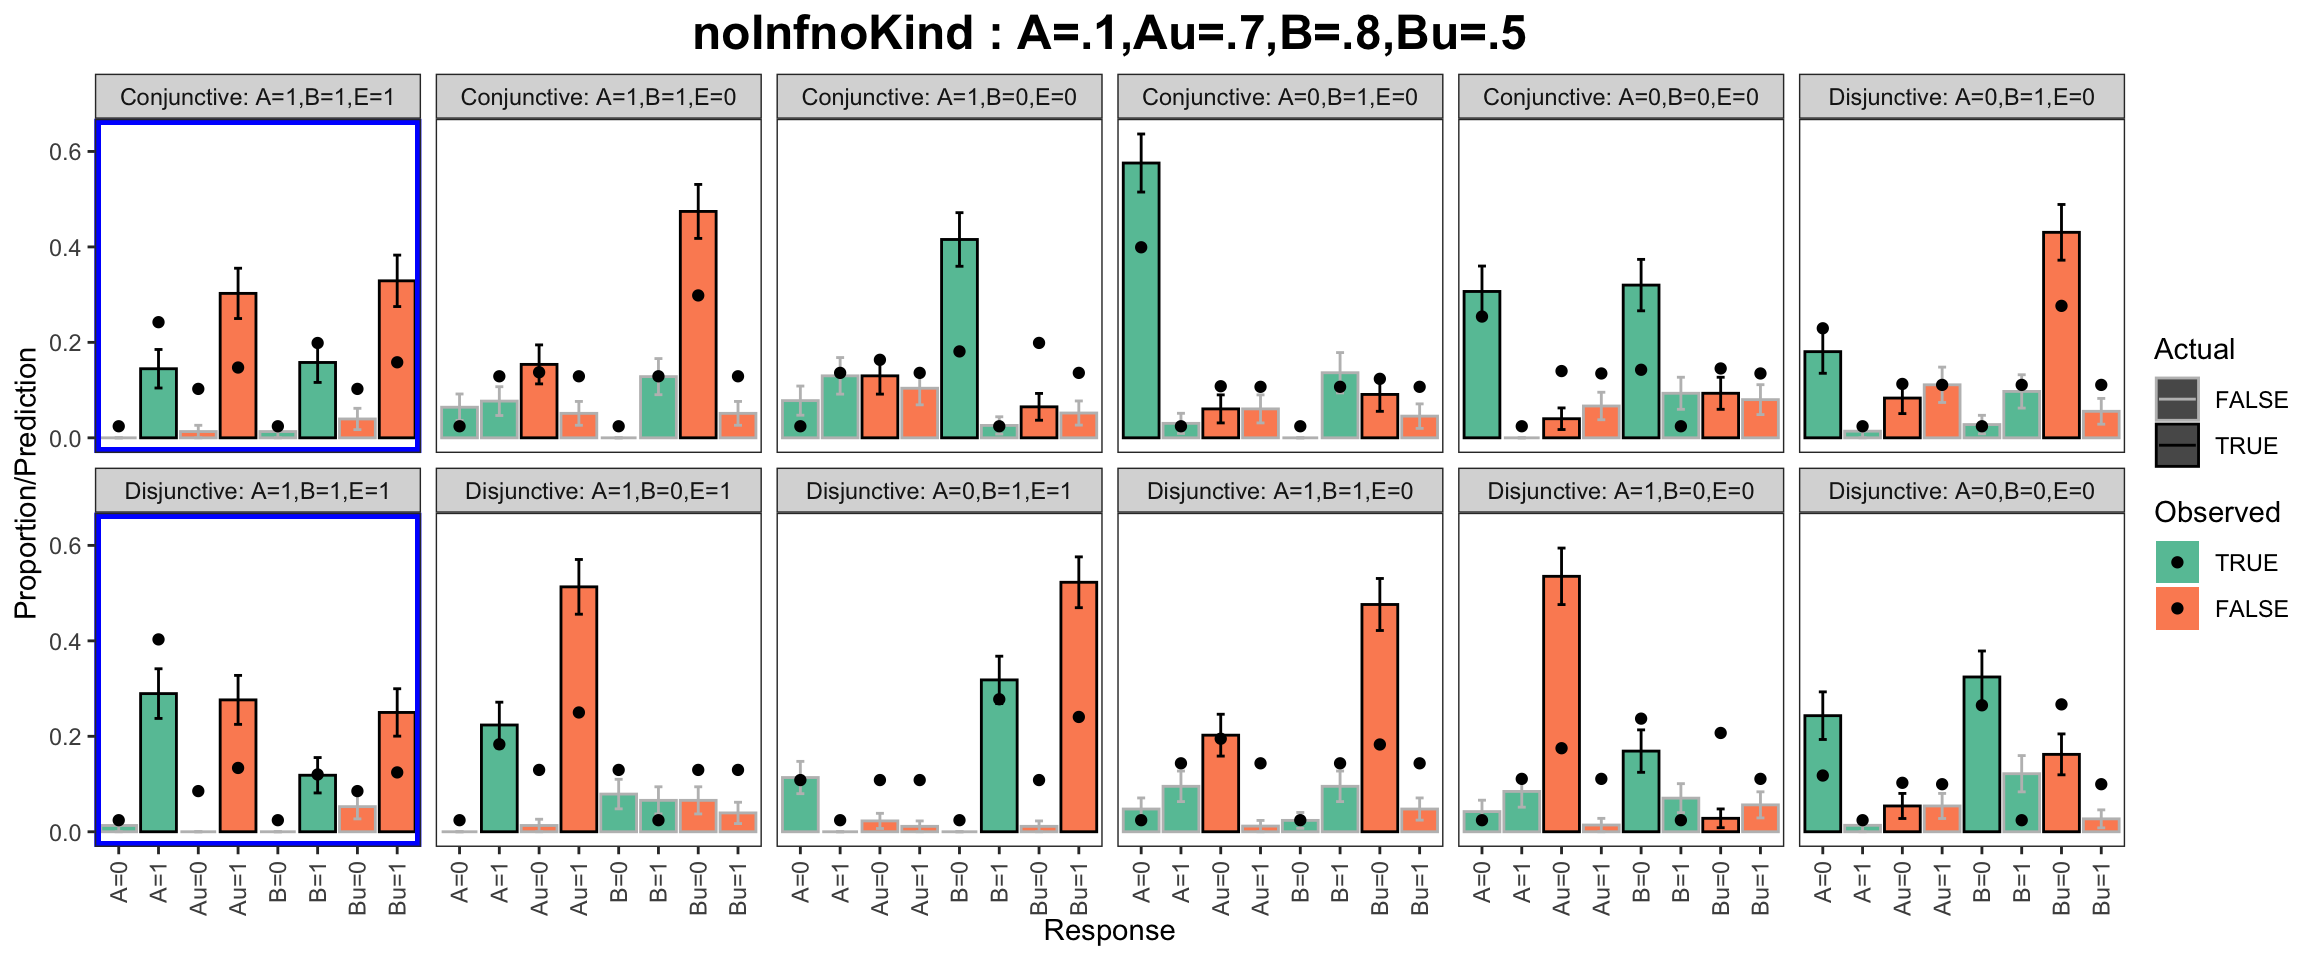
\includegraphics[keepaspectratio]{reportingFigs16m_files/figure-latex/unnamed-chunk-7-33.pdf}}
\pandocbounded{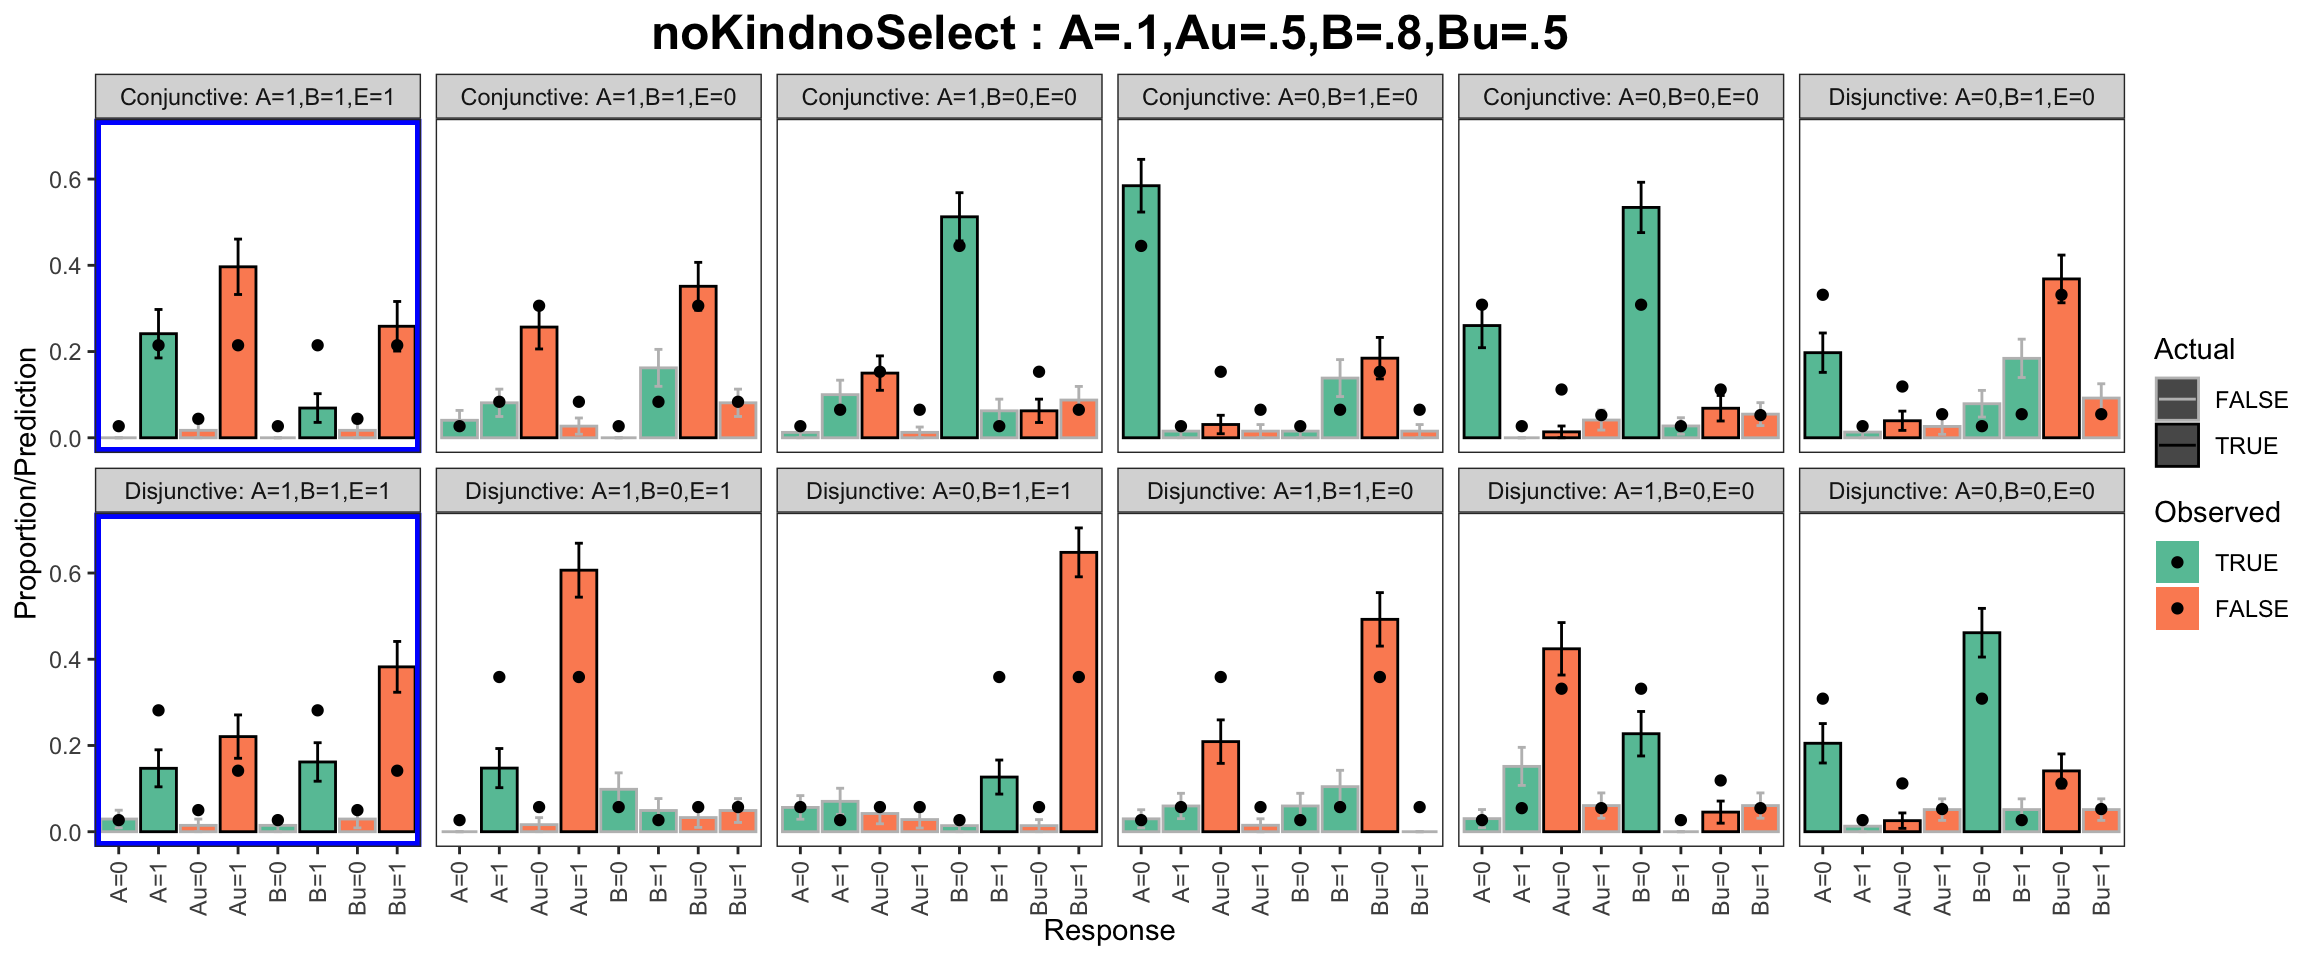
\includegraphics[keepaspectratio]{reportingFigs16m_files/figure-latex/unnamed-chunk-7-34.pdf}}
\pandocbounded{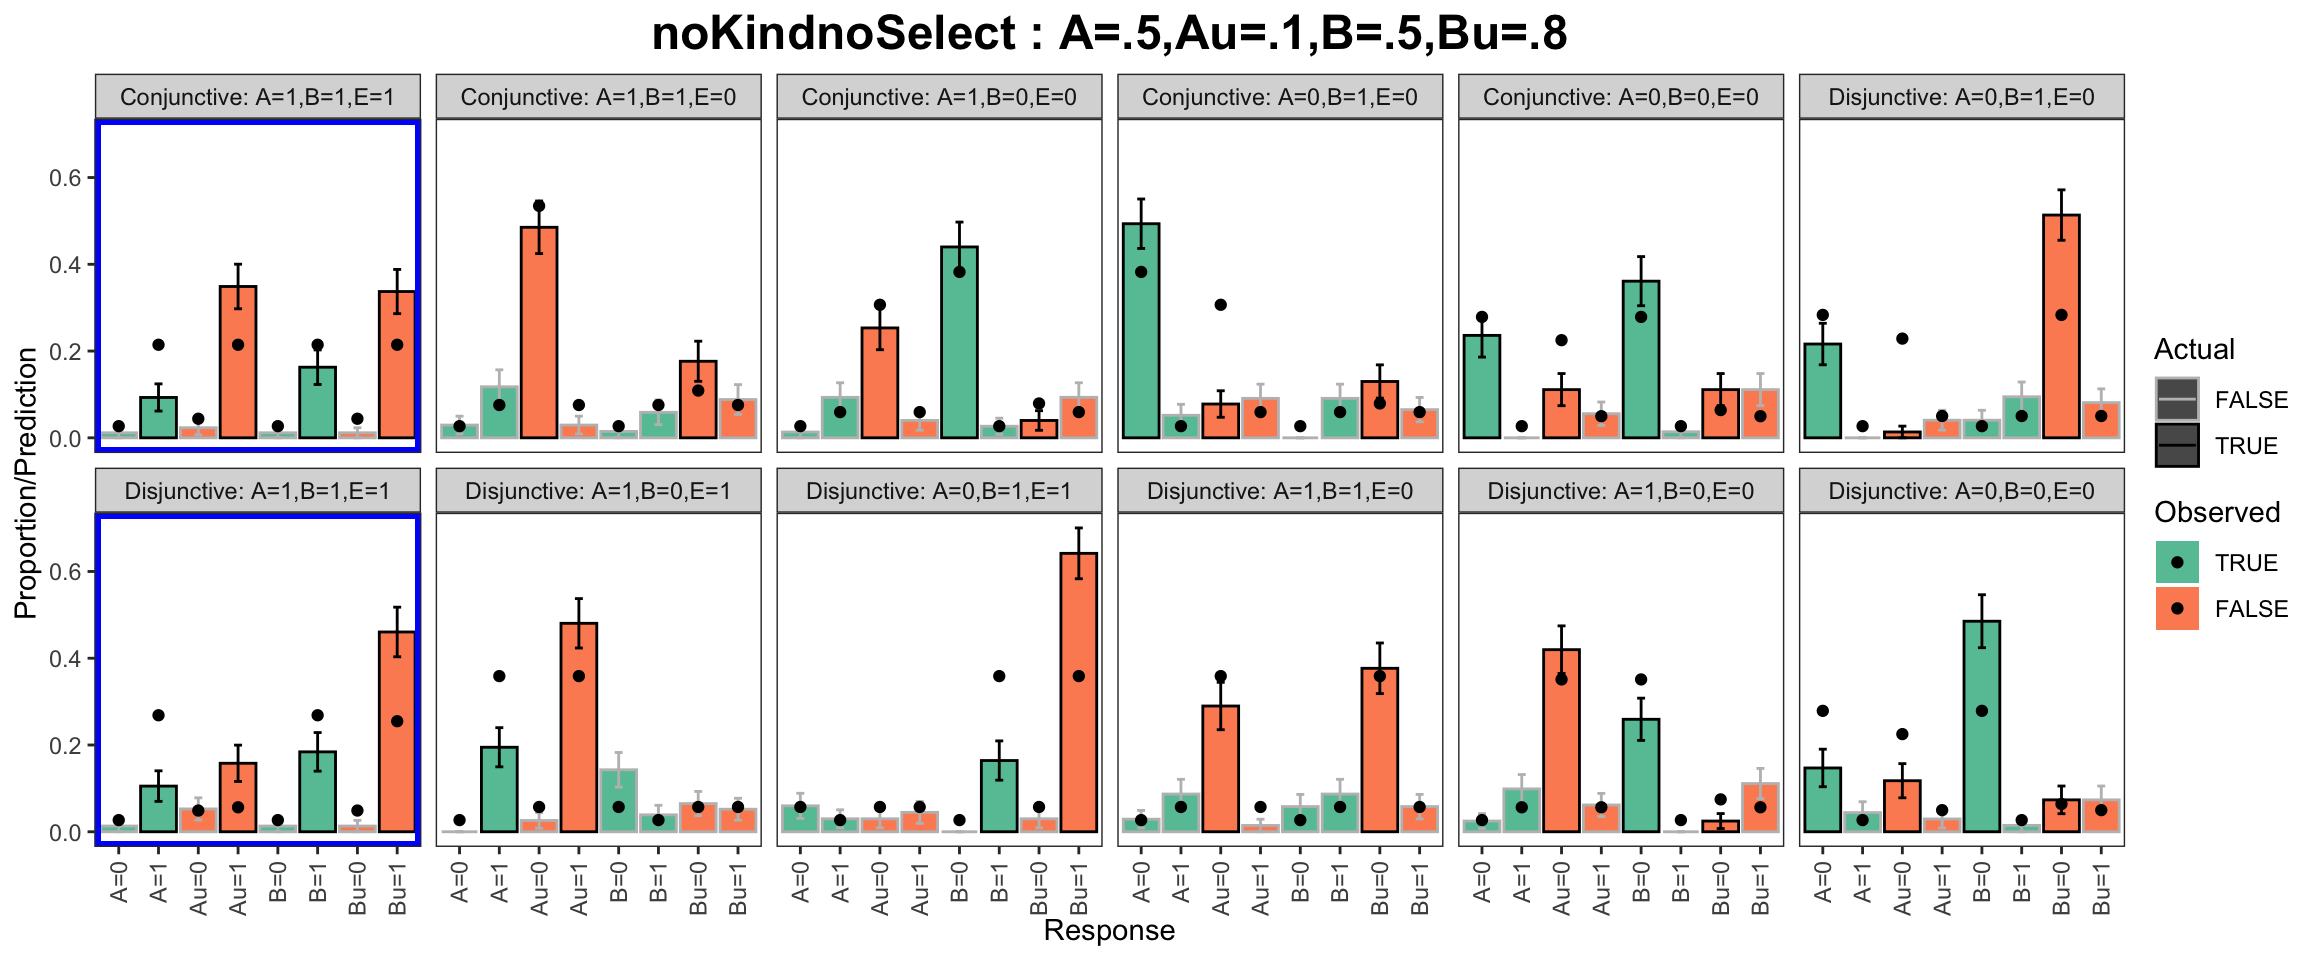
\includegraphics[keepaspectratio]{reportingFigs16m_files/figure-latex/unnamed-chunk-7-35.pdf}}
\pandocbounded{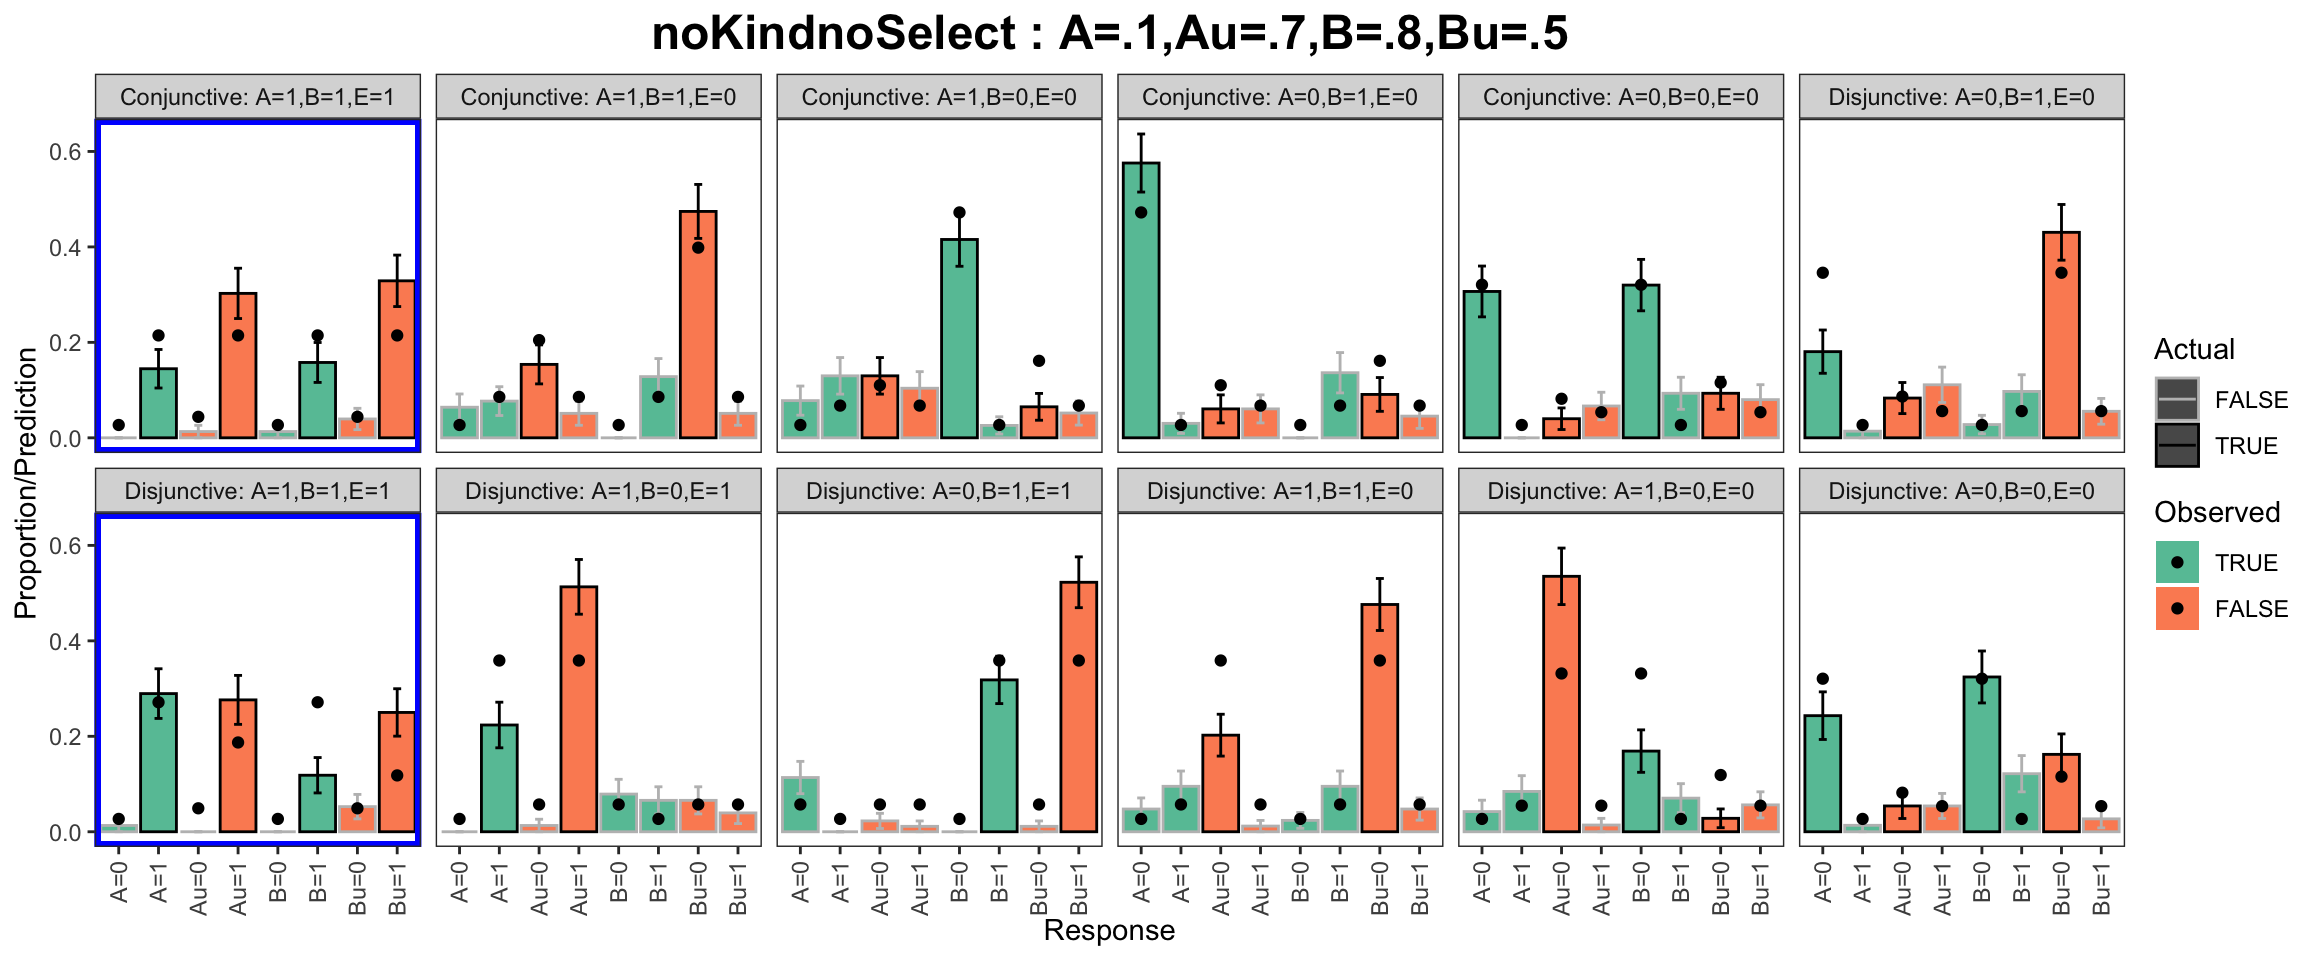
\includegraphics[keepaspectratio]{reportingFigs16m_files/figure-latex/unnamed-chunk-7-36.pdf}}
\pandocbounded{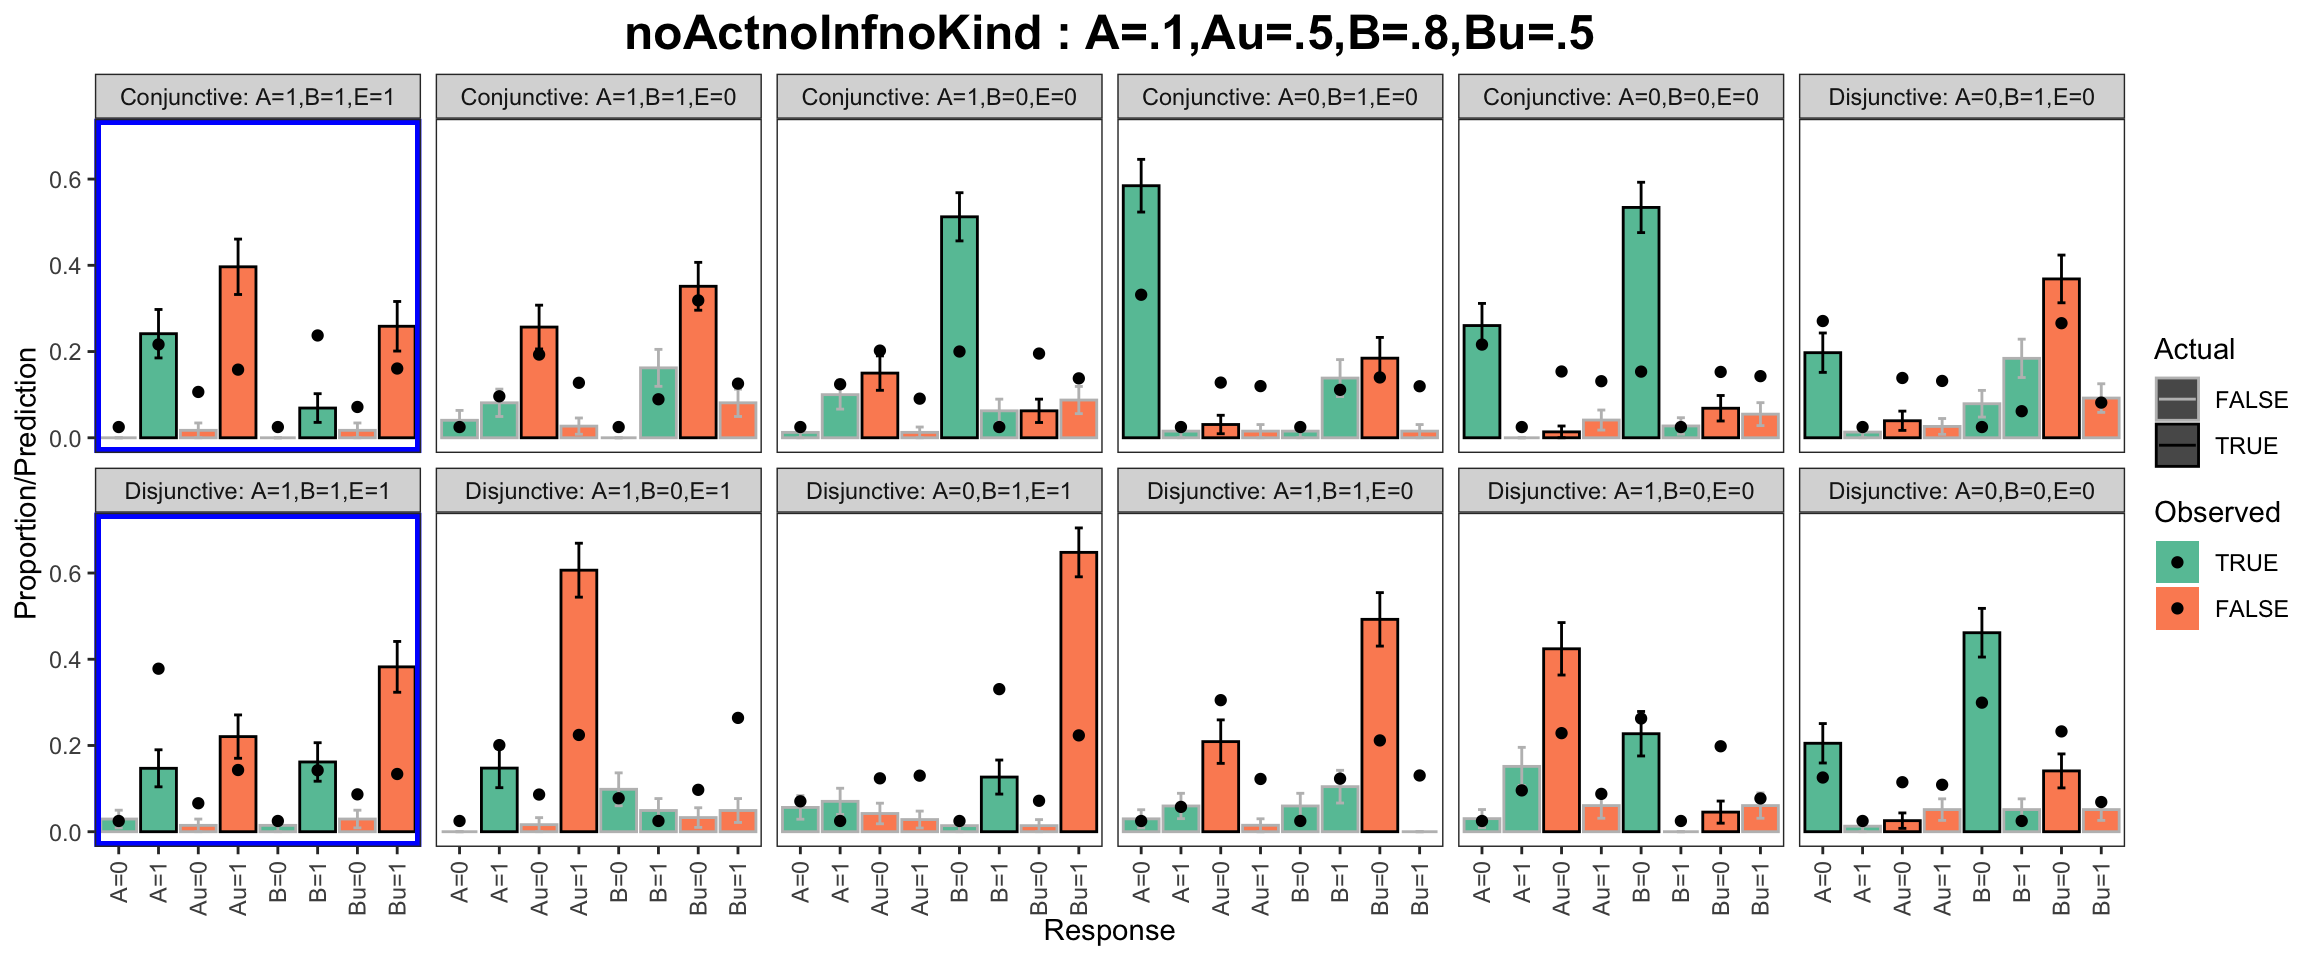
\includegraphics[keepaspectratio]{reportingFigs16m_files/figure-latex/unnamed-chunk-7-37.pdf}}
\pandocbounded{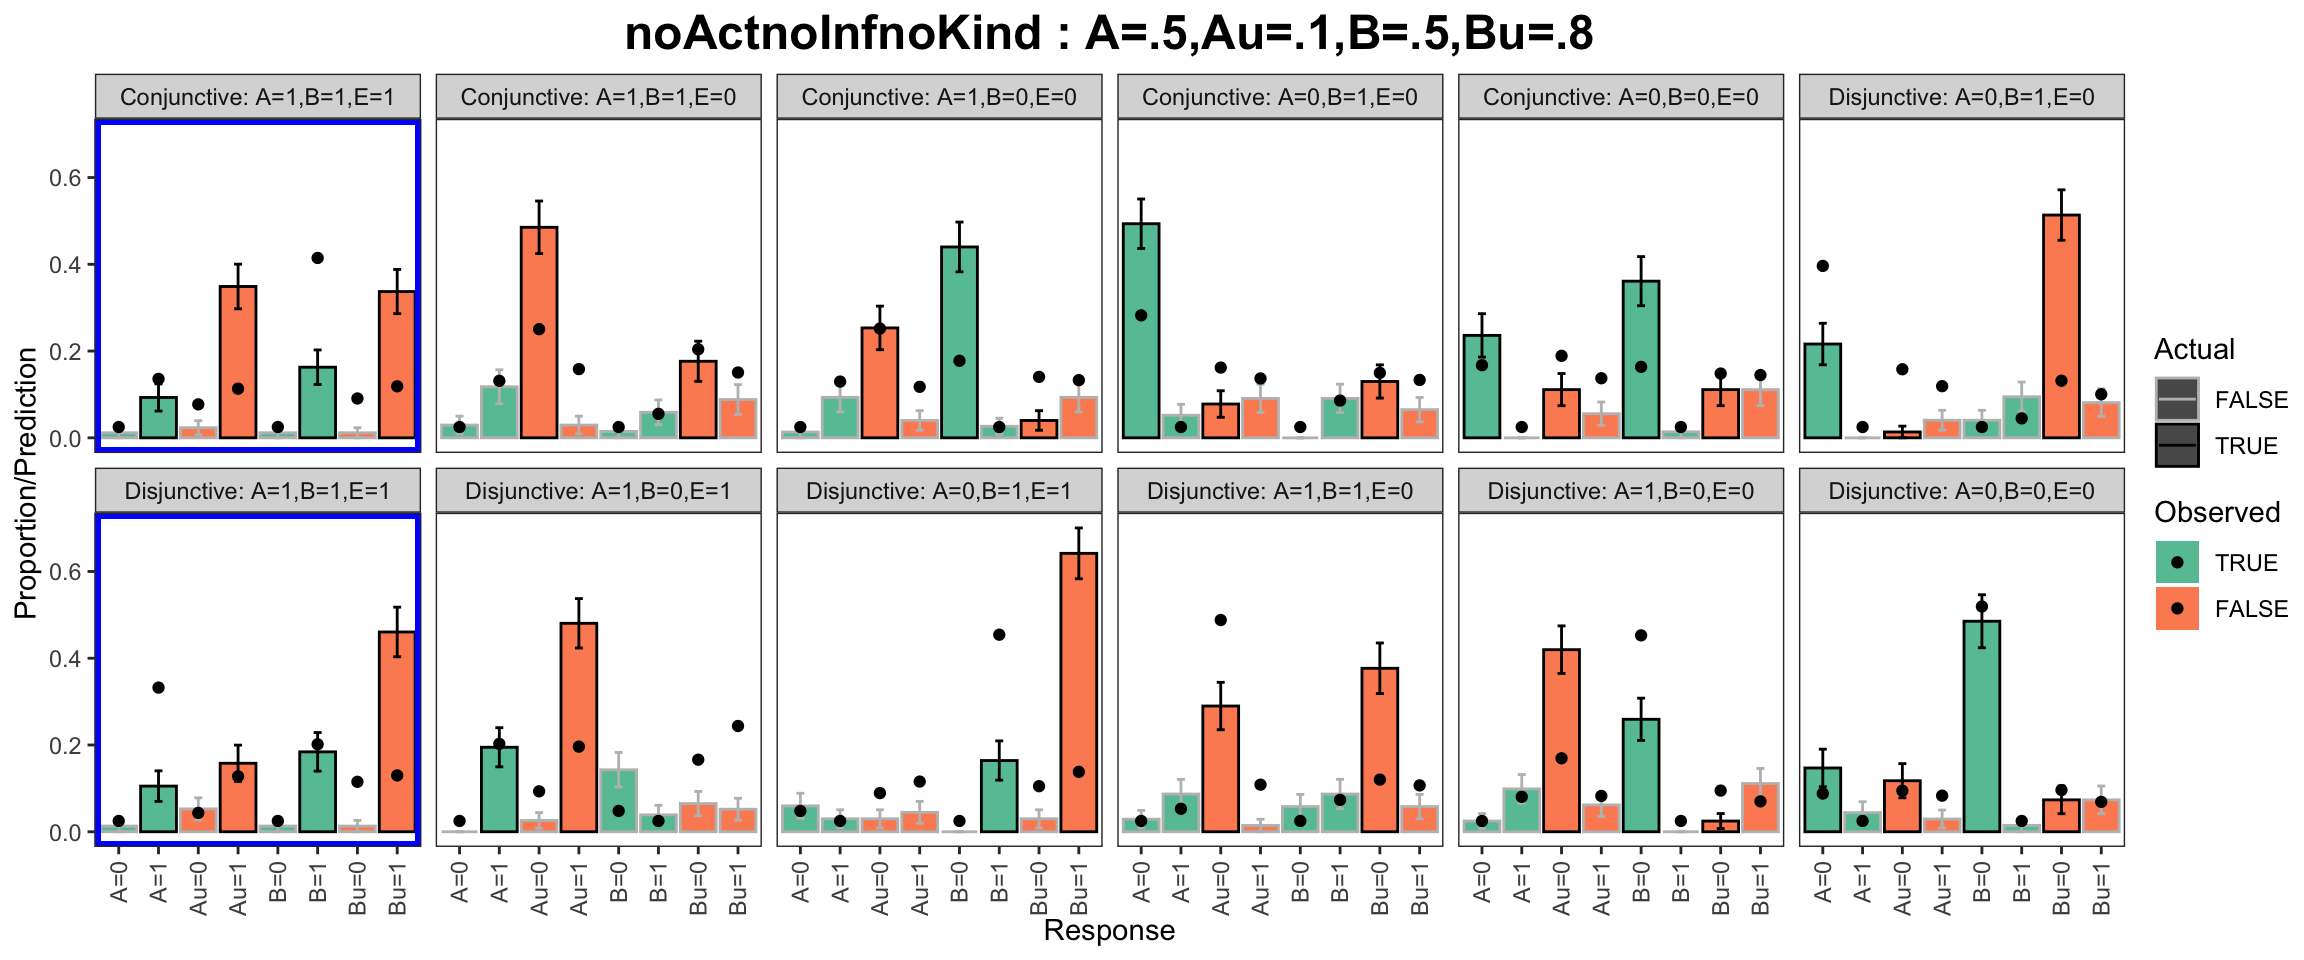
\includegraphics[keepaspectratio]{reportingFigs16m_files/figure-latex/unnamed-chunk-7-38.pdf}}
\pandocbounded{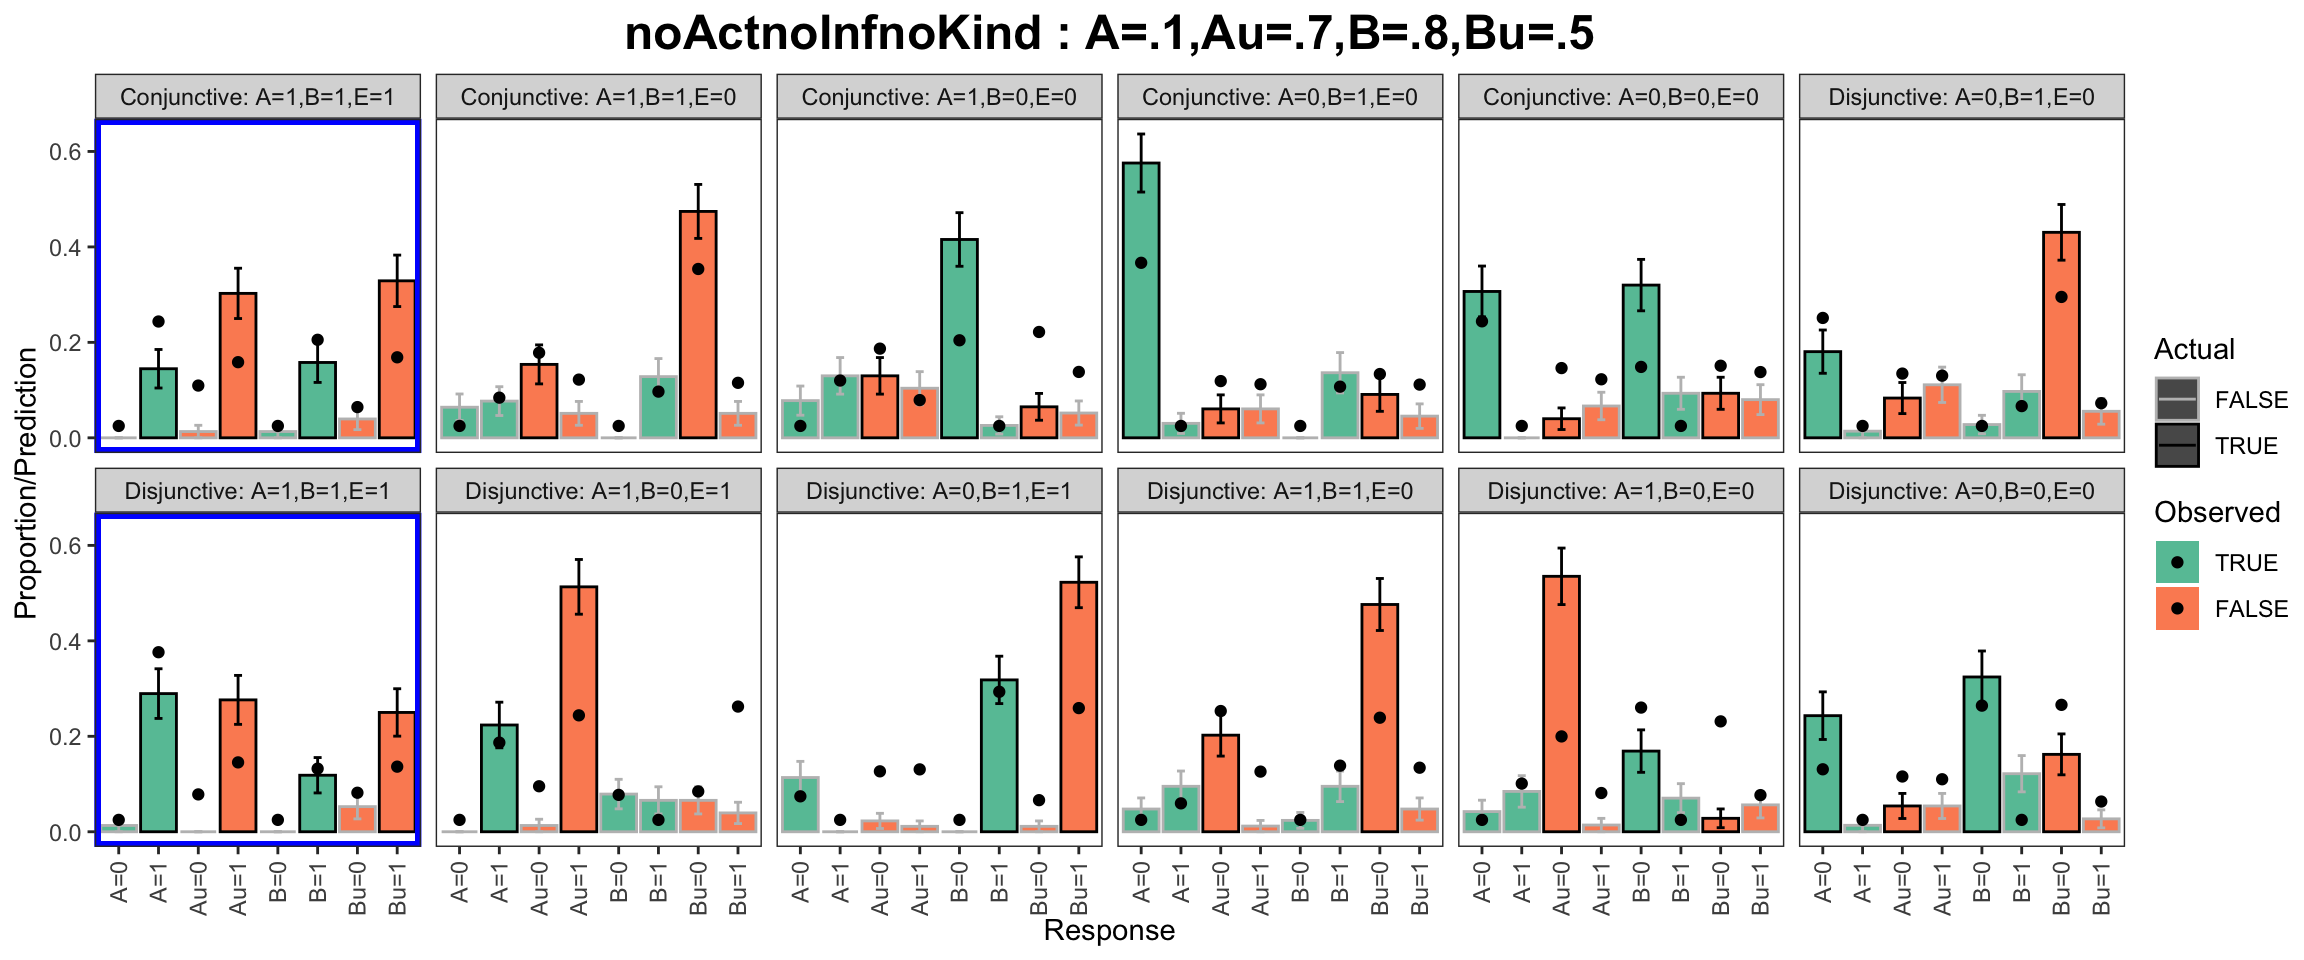
\includegraphics[keepaspectratio]{reportingFigs16m_files/figure-latex/unnamed-chunk-7-39.pdf}}
\pandocbounded{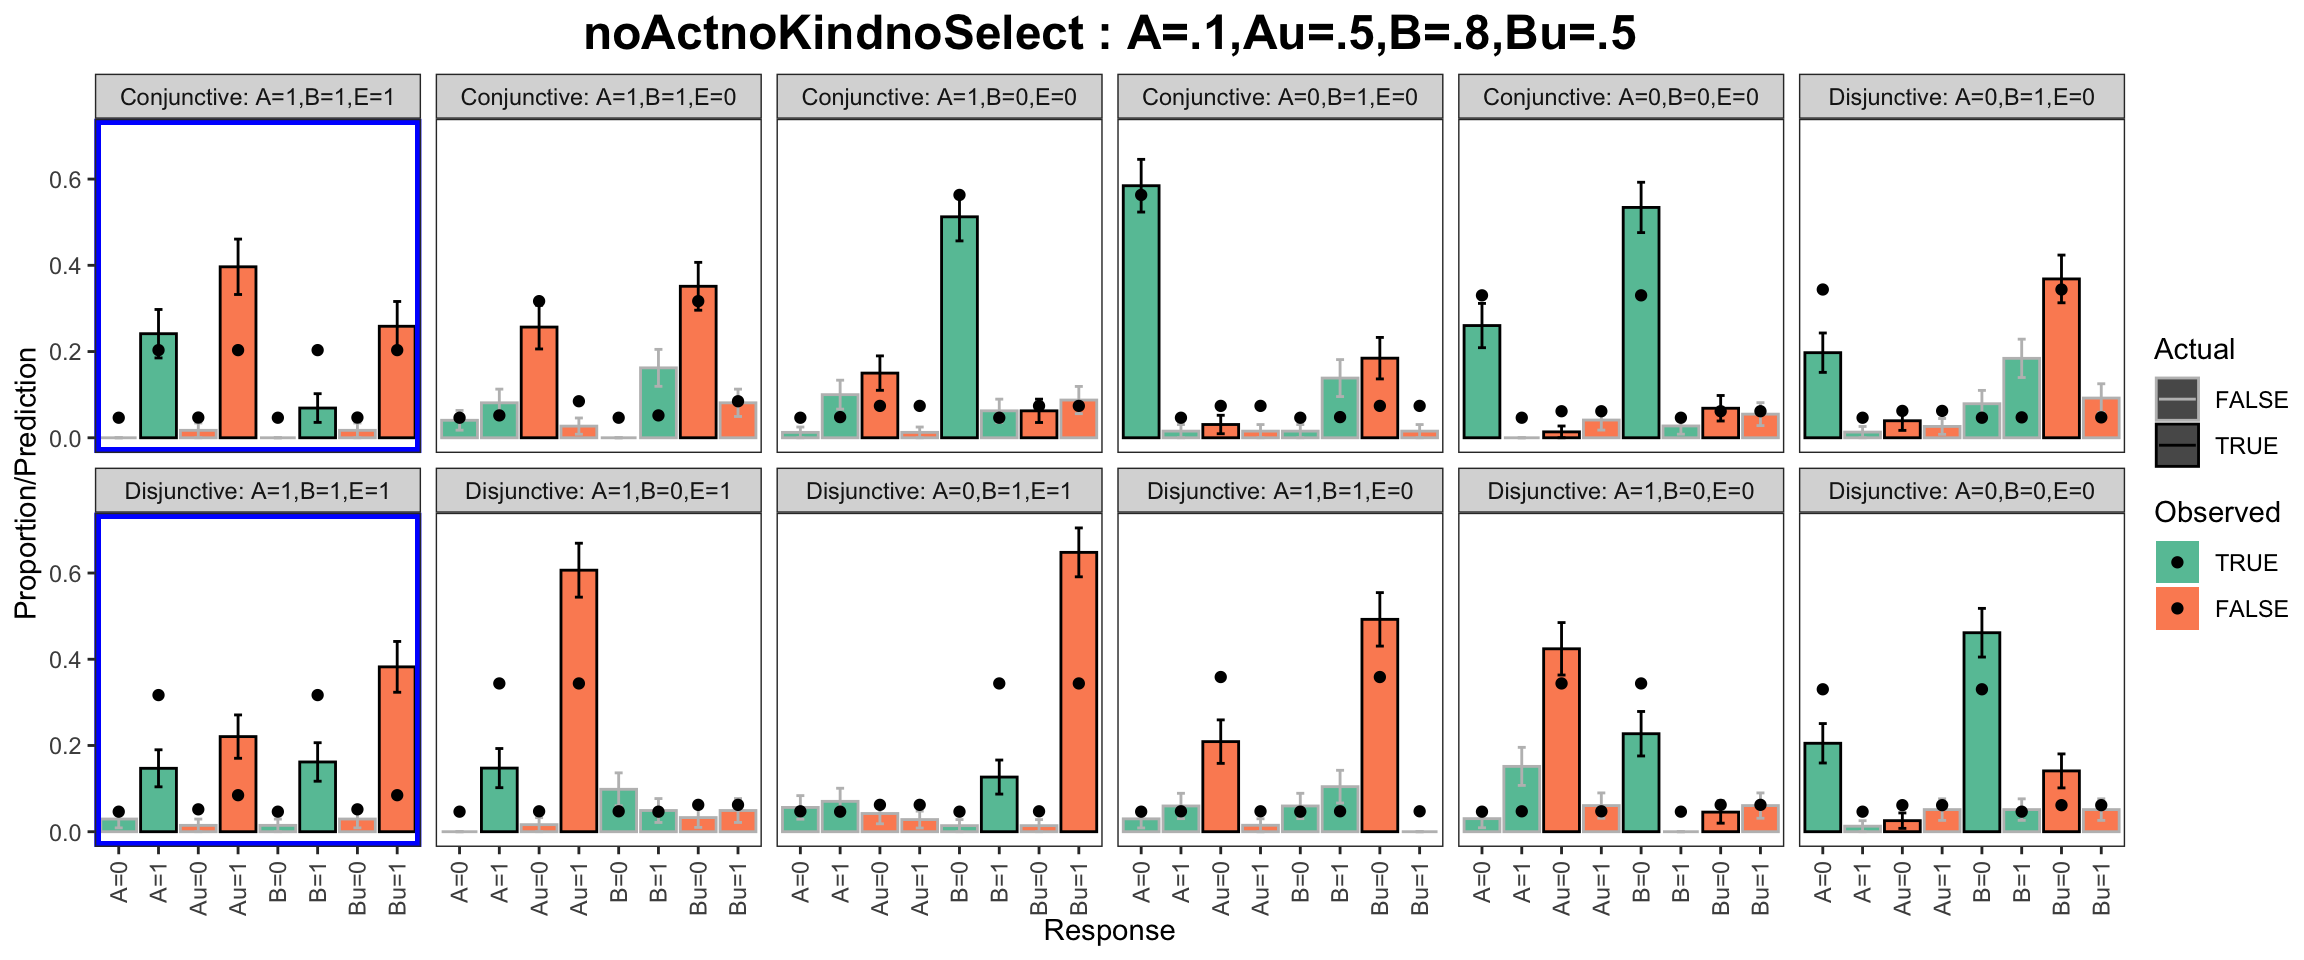
\includegraphics[keepaspectratio]{reportingFigs16m_files/figure-latex/unnamed-chunk-7-40.pdf}}
\pandocbounded{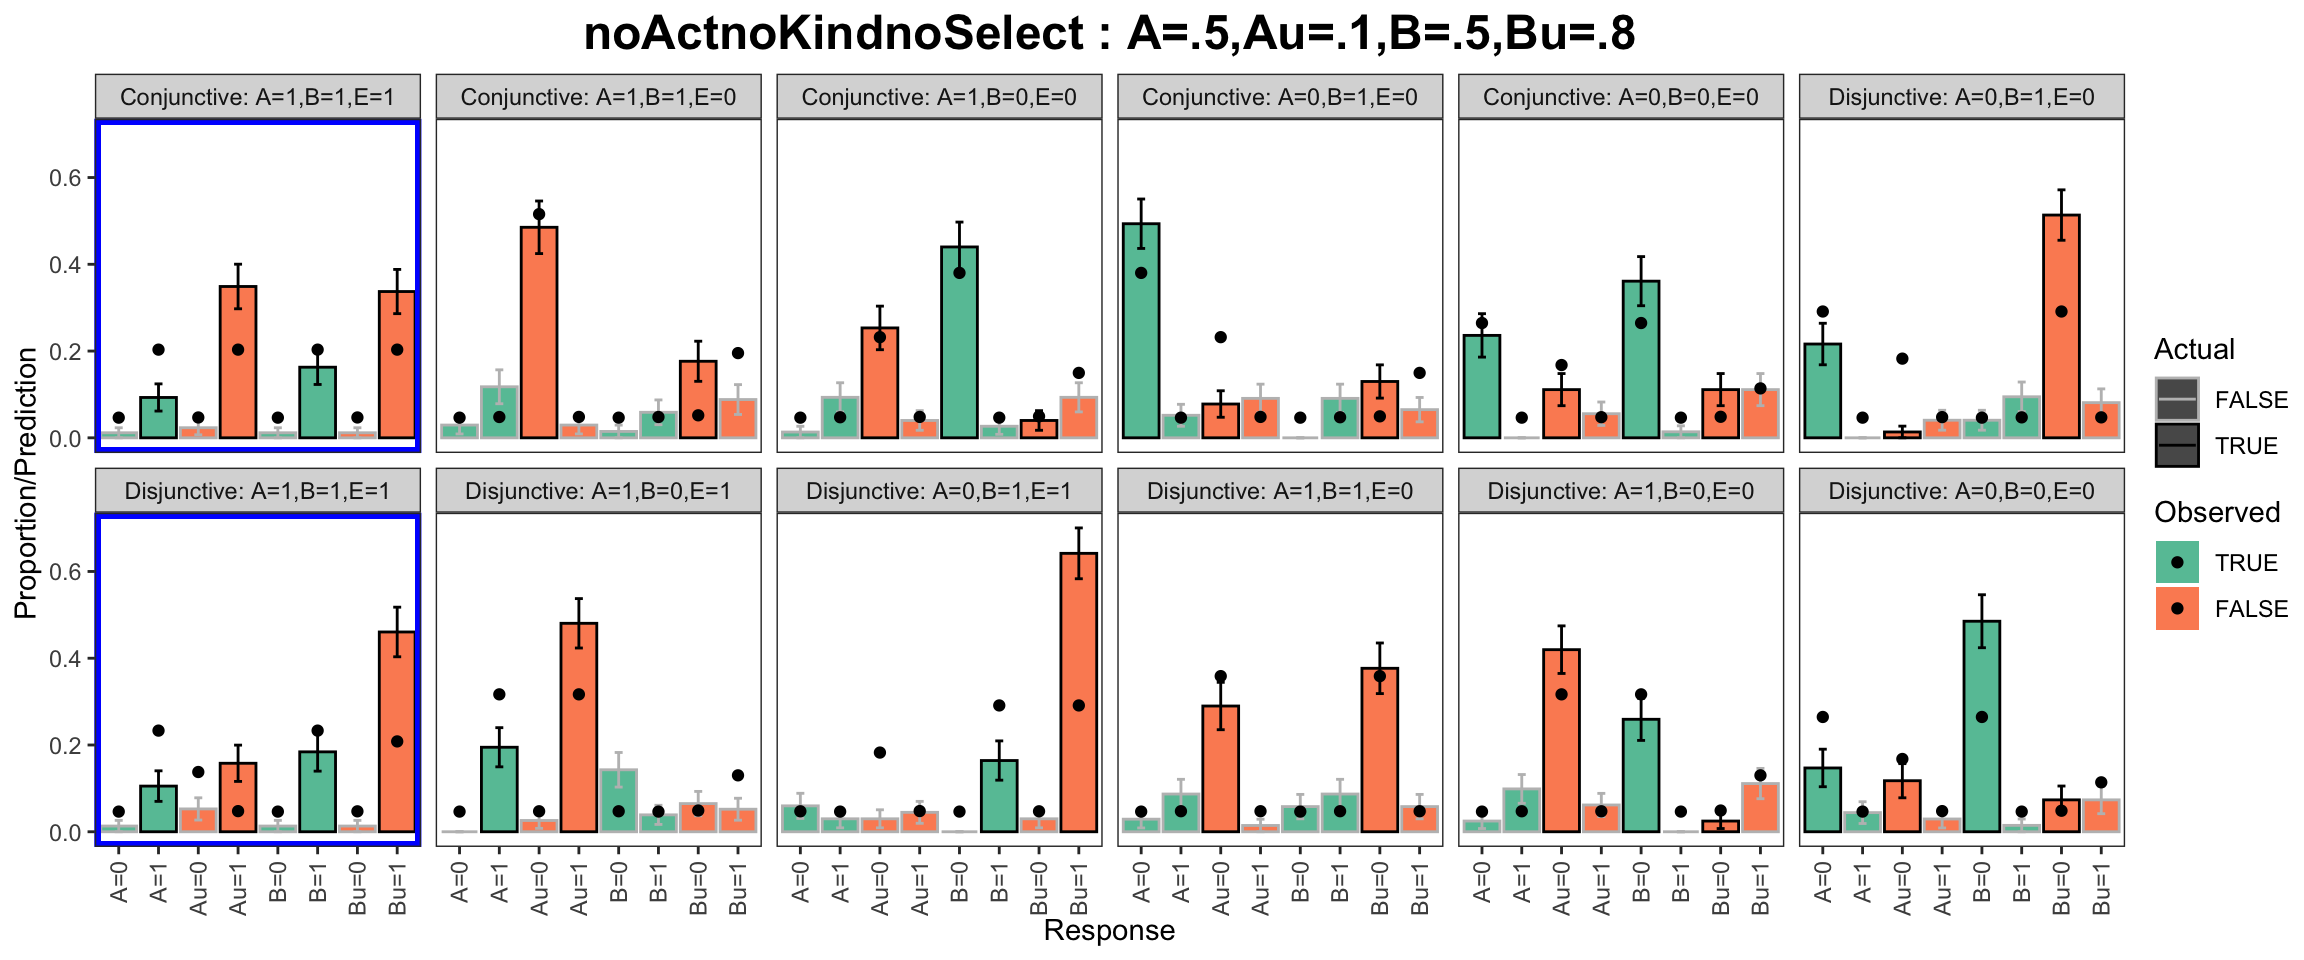
\includegraphics[keepaspectratio]{reportingFigs16m_files/figure-latex/unnamed-chunk-7-41.pdf}}
\pandocbounded{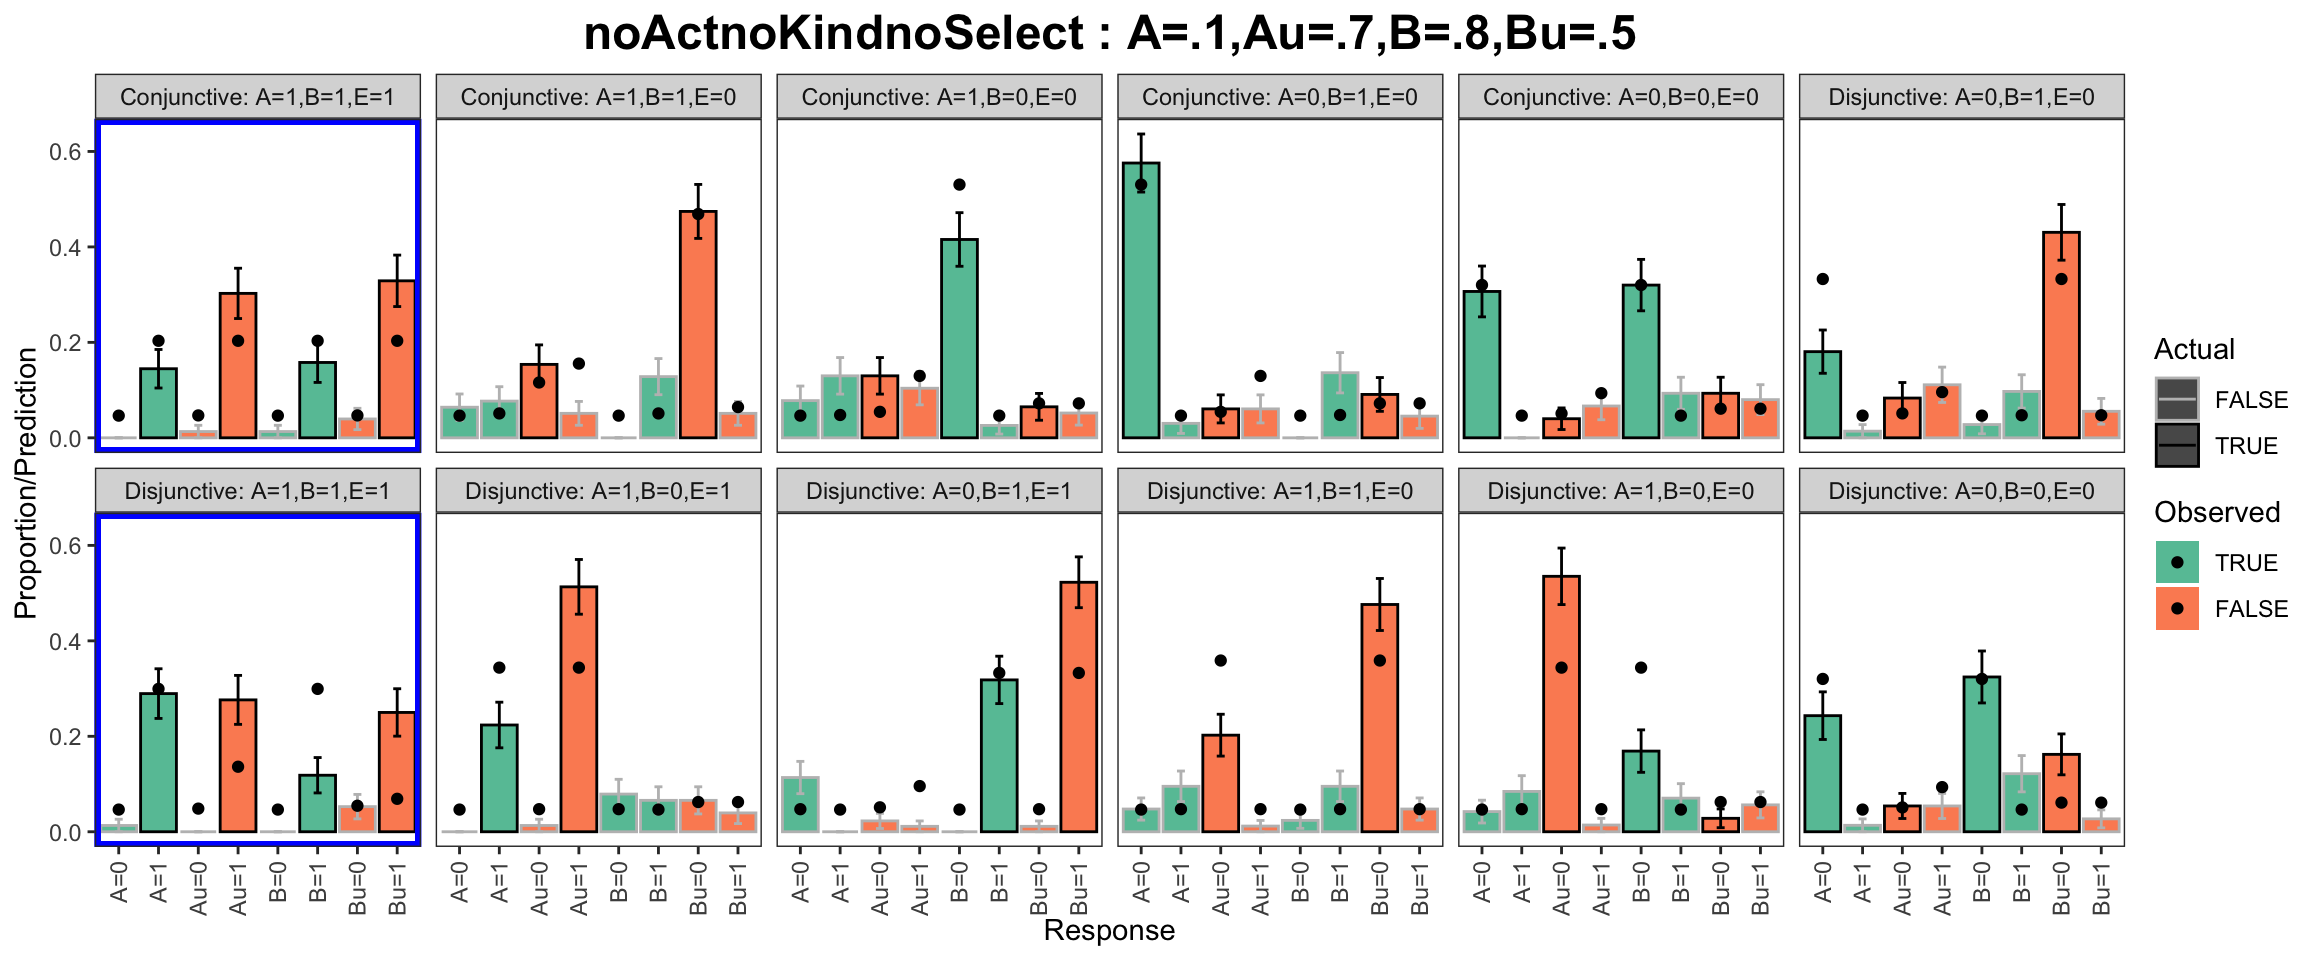
\includegraphics[keepaspectratio]{reportingFigs16m_files/figure-latex/unnamed-chunk-7-42.pdf}}
\pandocbounded{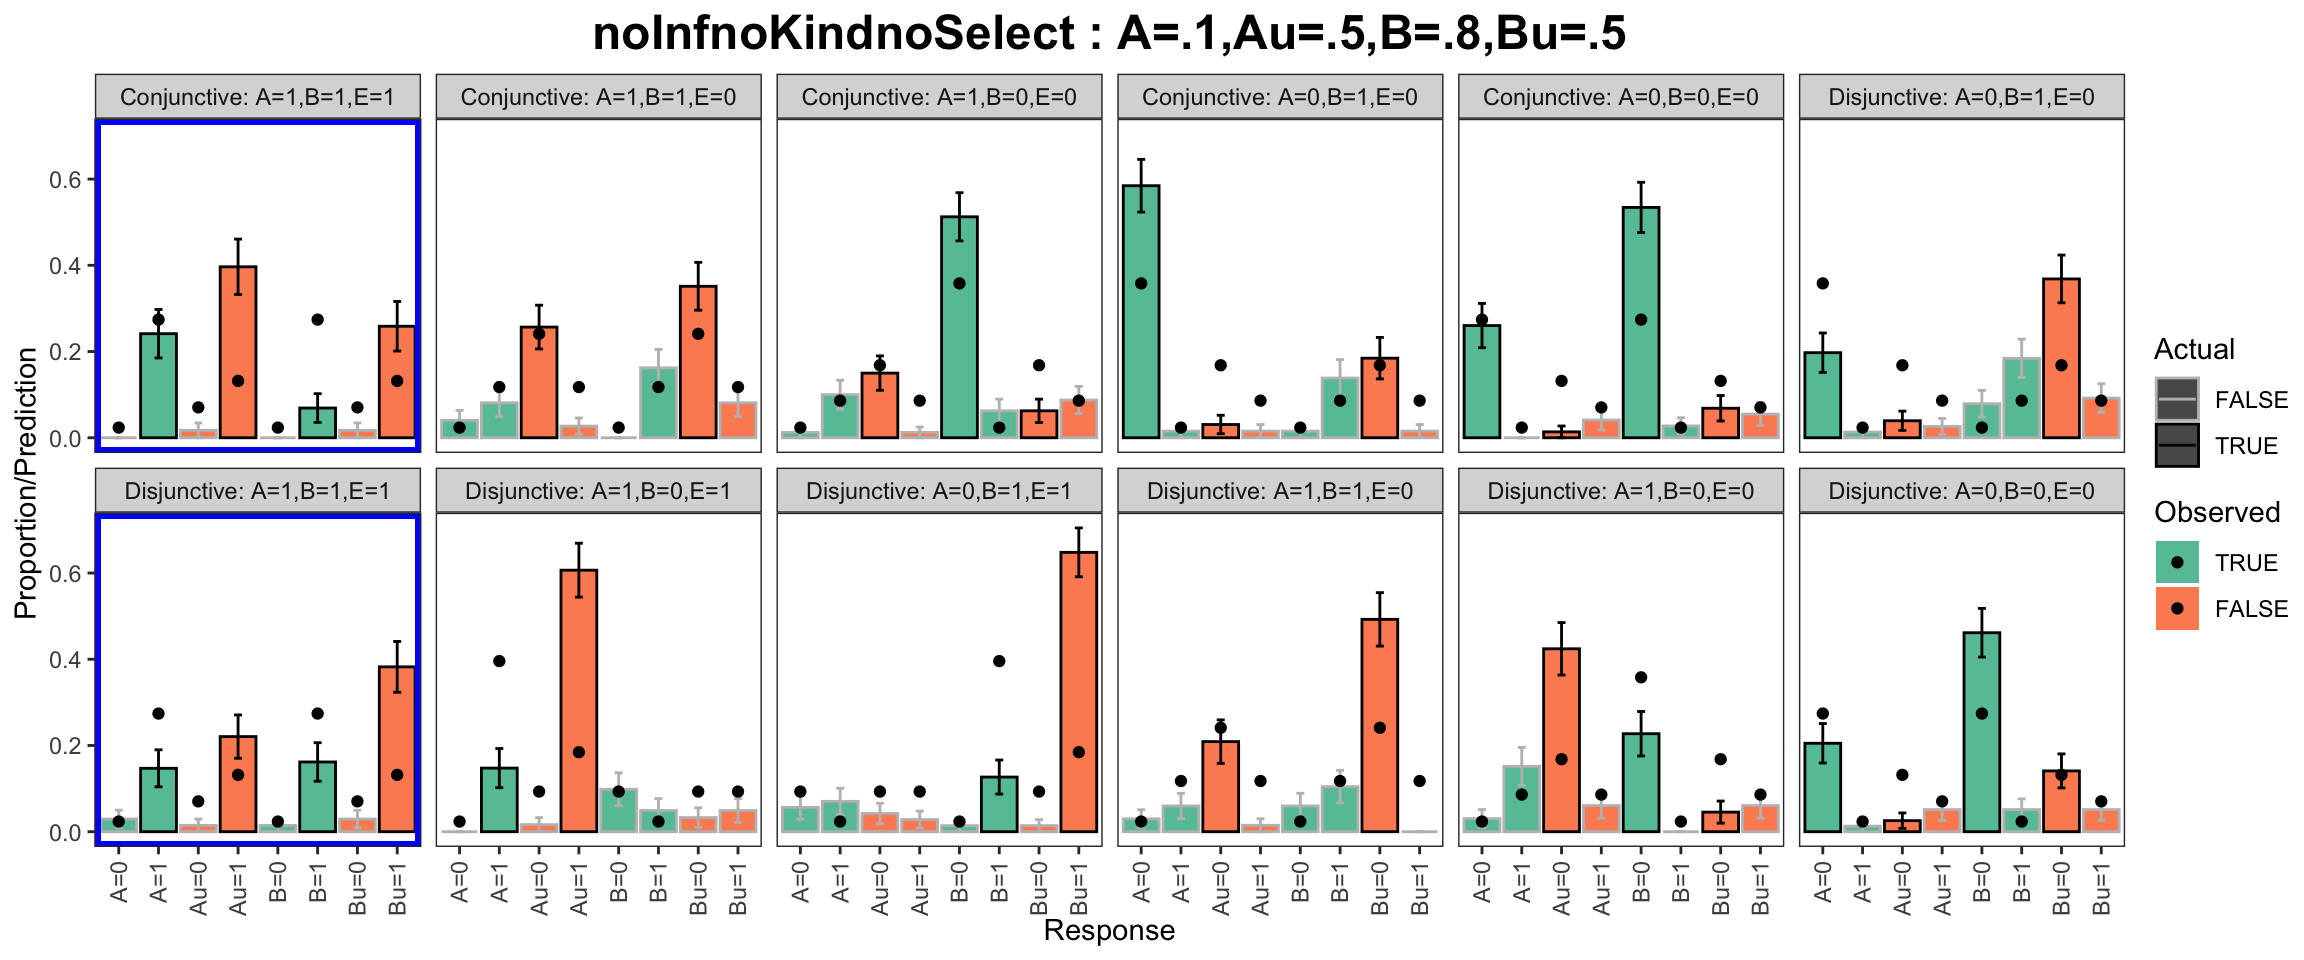
\includegraphics[keepaspectratio]{reportingFigs16m_files/figure-latex/unnamed-chunk-7-43.pdf}}
\pandocbounded{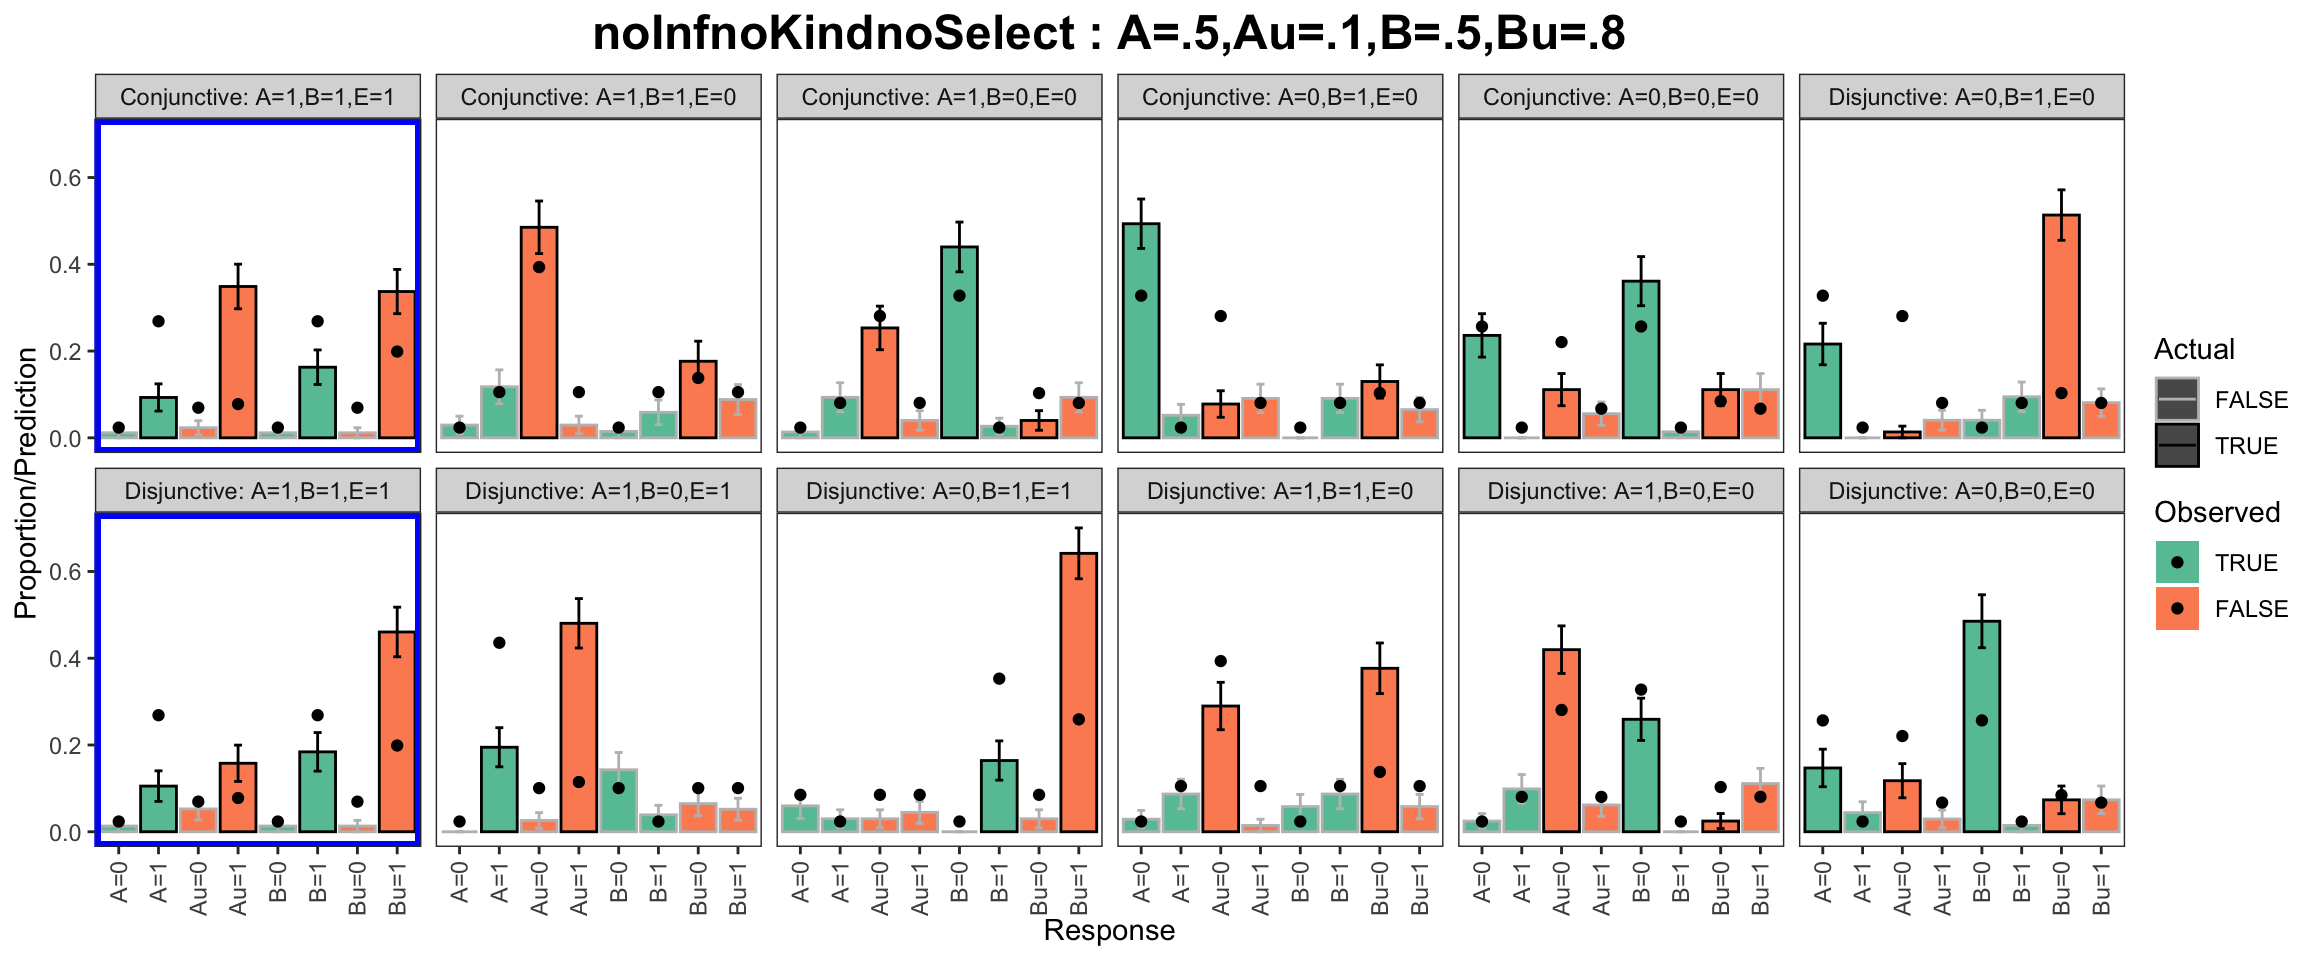
\includegraphics[keepaspectratio]{reportingFigs16m_files/figure-latex/unnamed-chunk-7-44.pdf}}
\pandocbounded{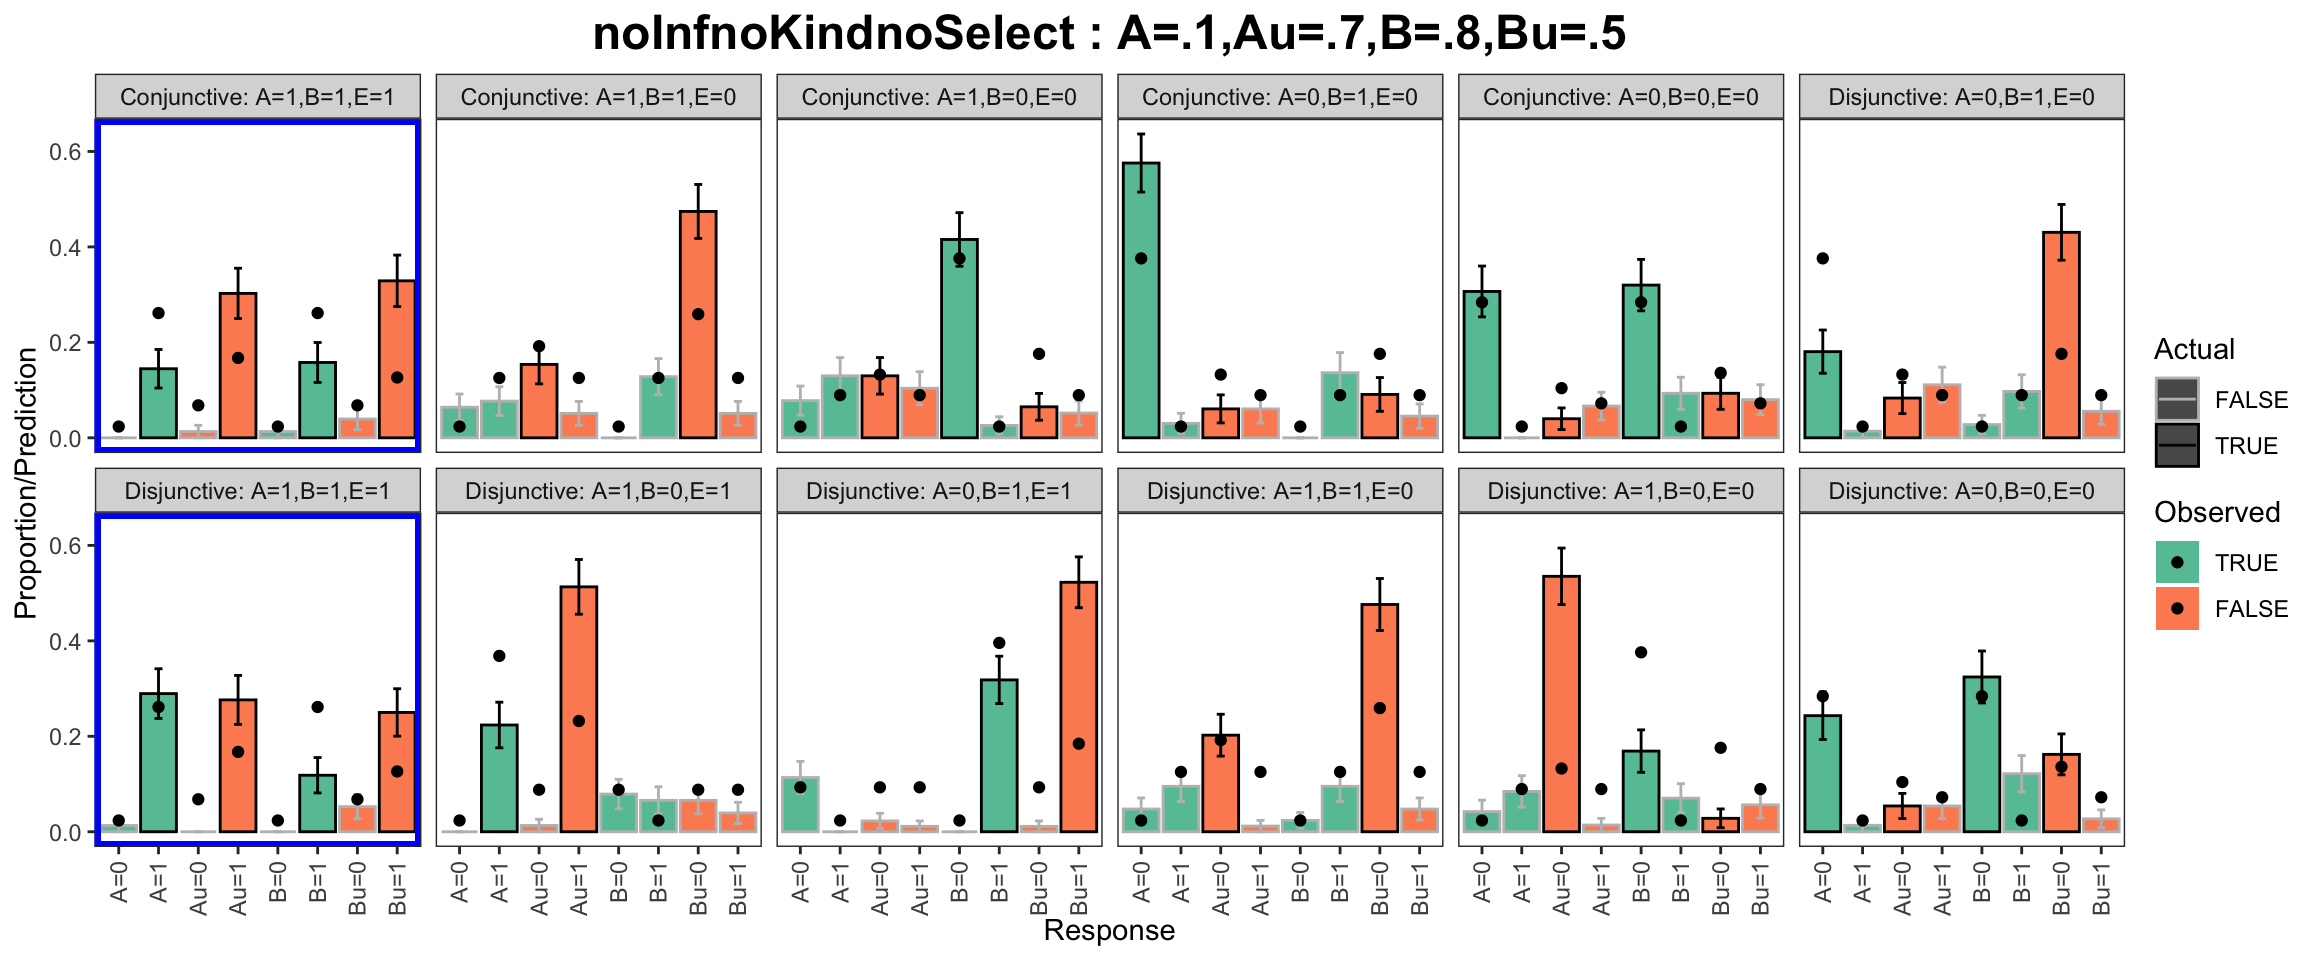
\includegraphics[keepaspectratio]{reportingFigs16m_files/figure-latex/unnamed-chunk-7-45.pdf}}
\pandocbounded{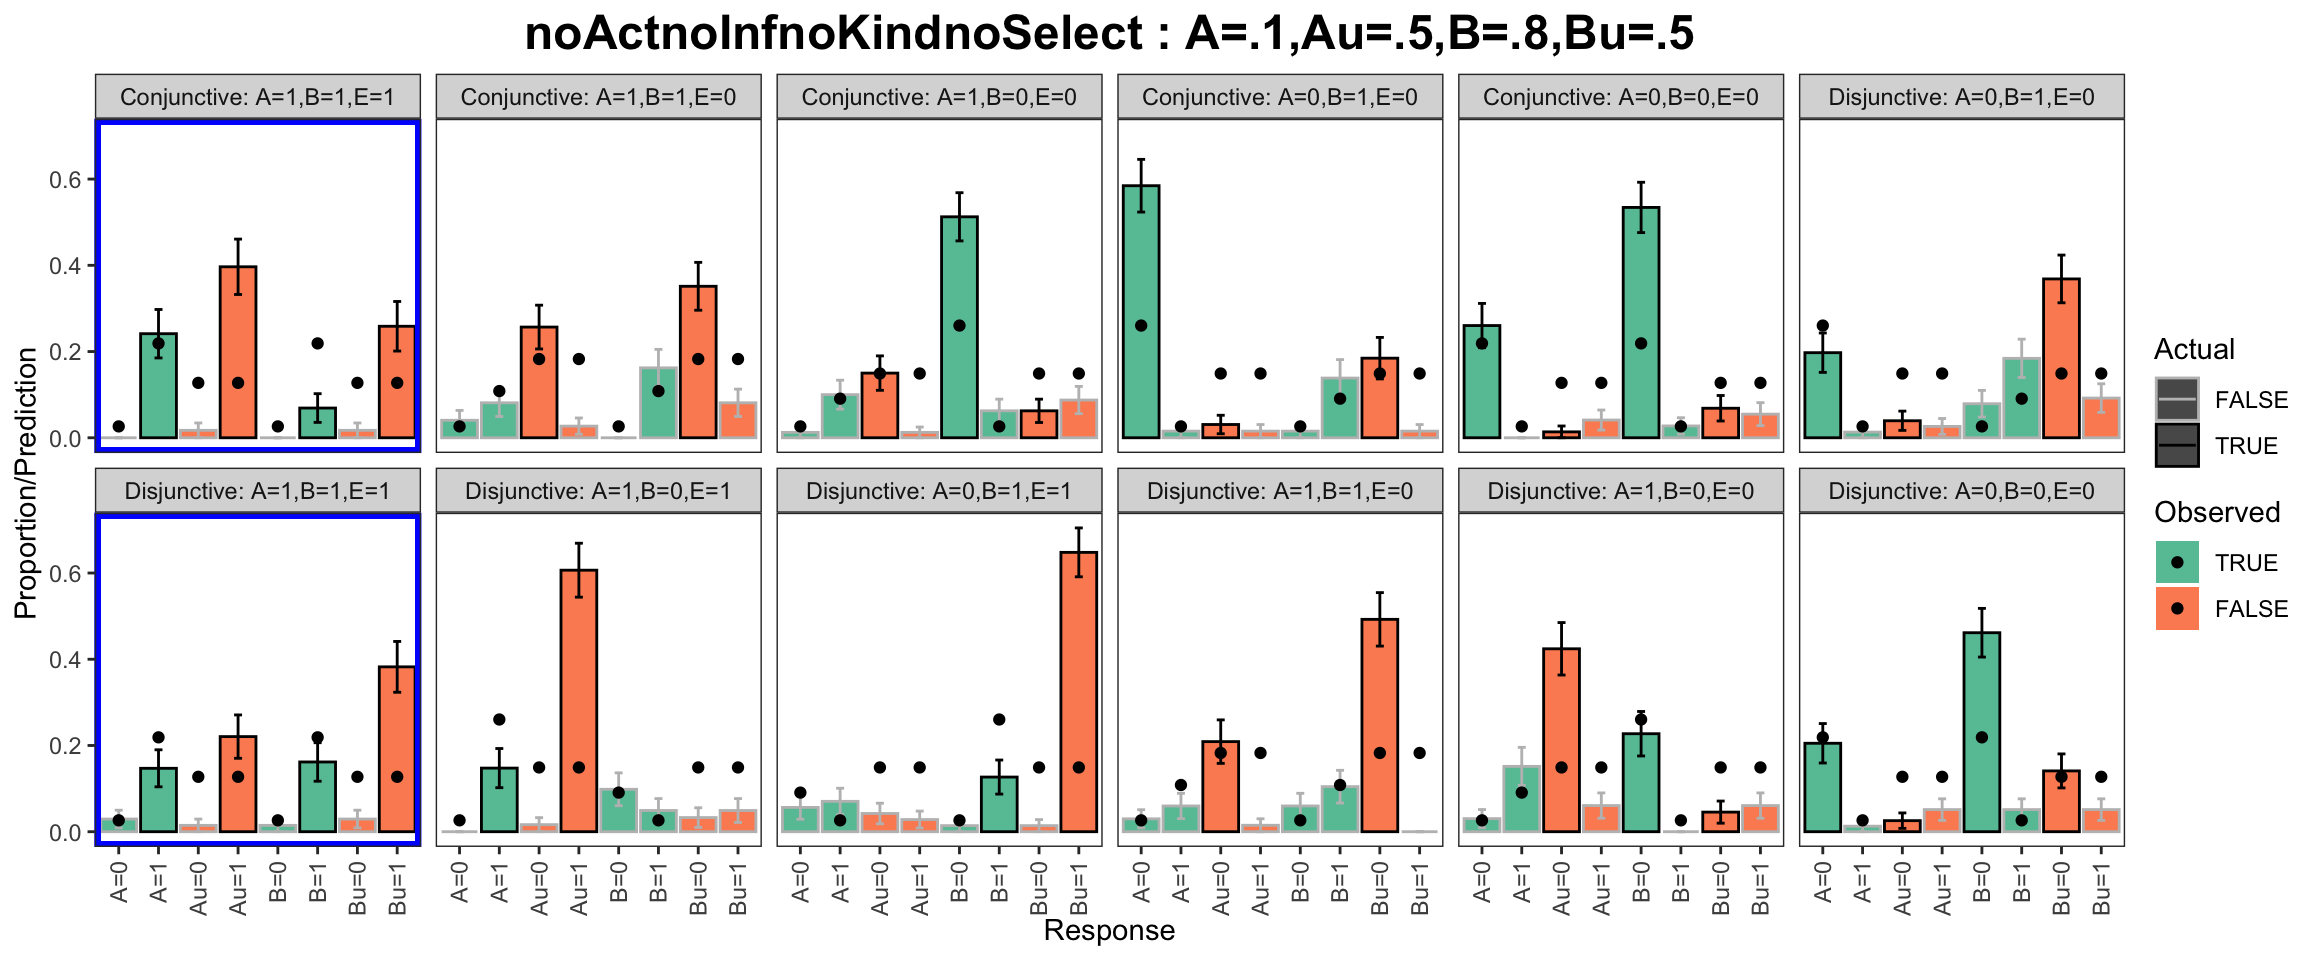
\includegraphics[keepaspectratio]{reportingFigs16m_files/figure-latex/unnamed-chunk-7-46.pdf}}
\pandocbounded{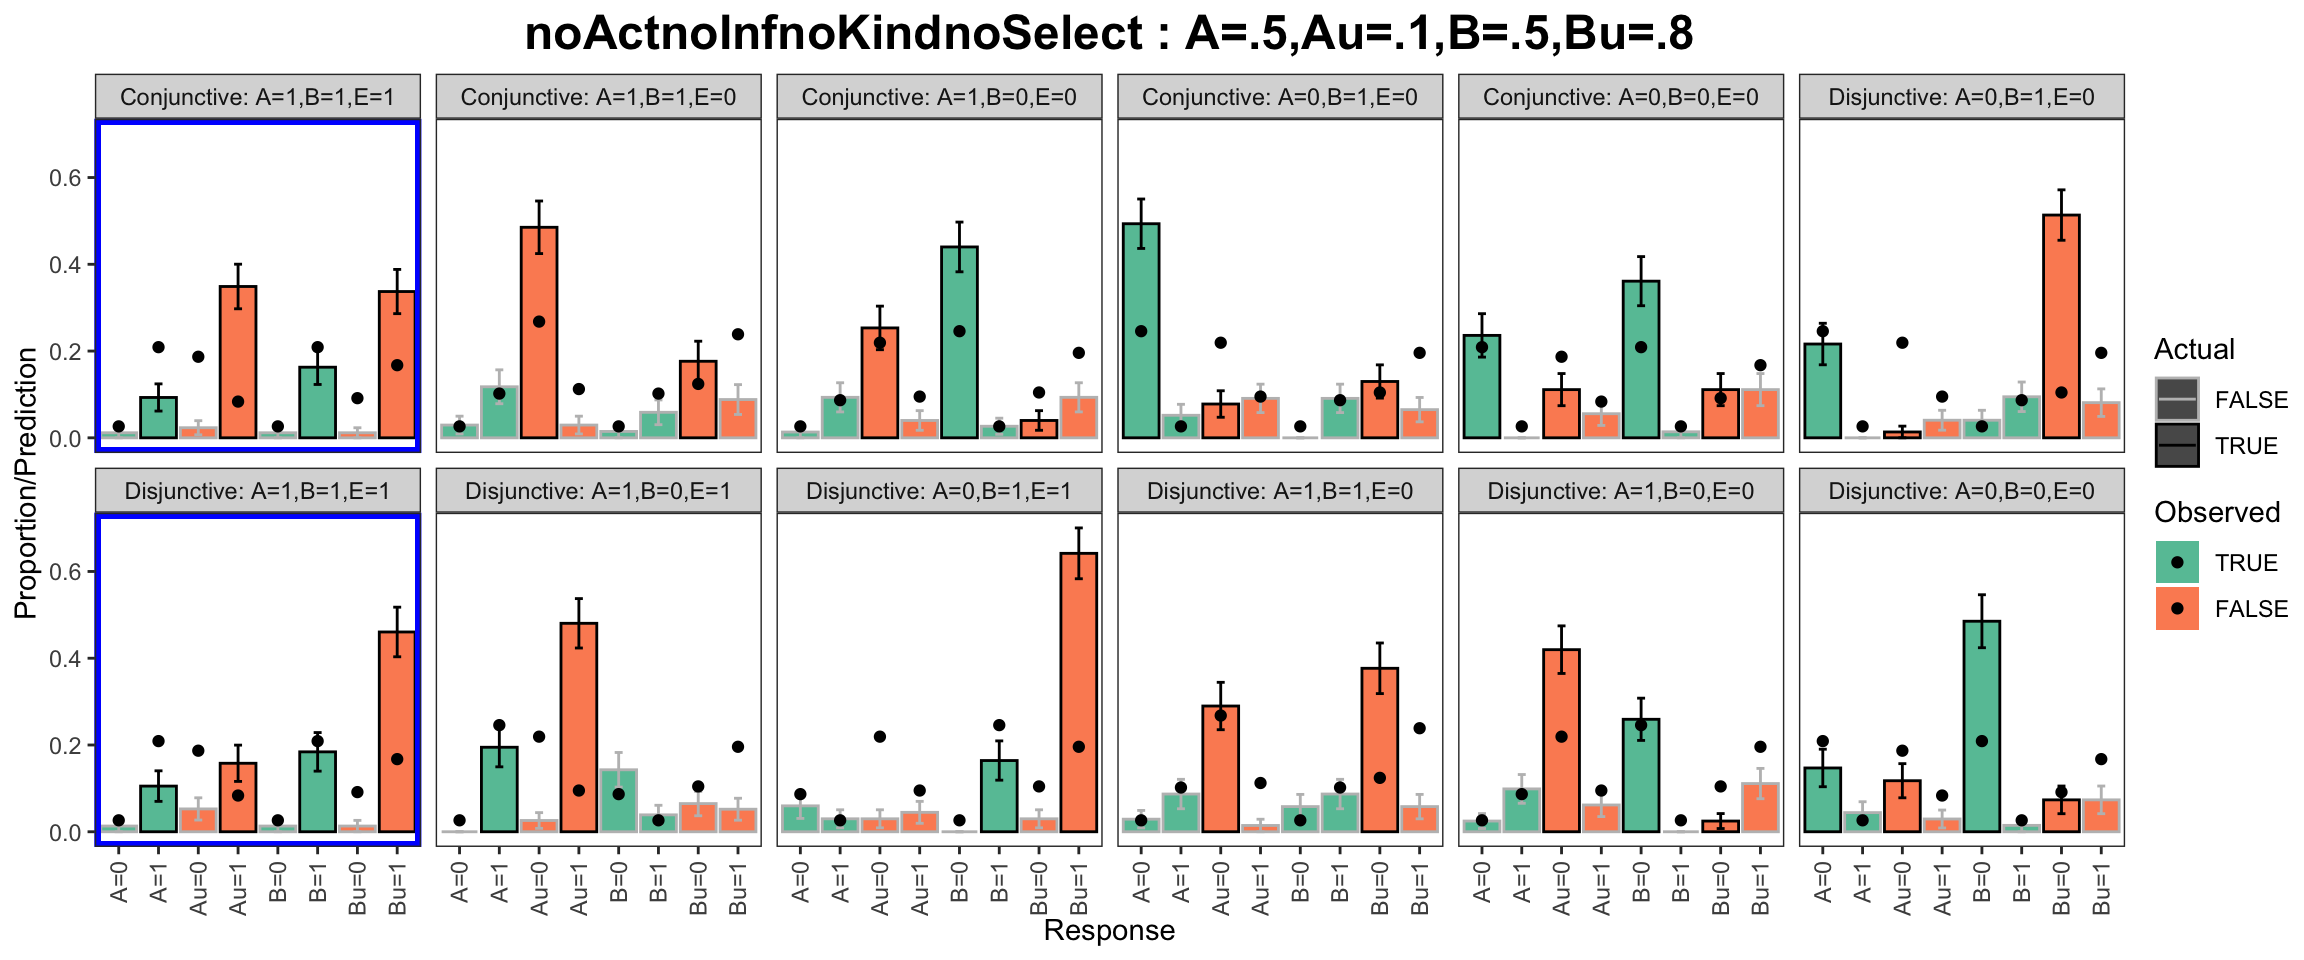
\includegraphics[keepaspectratio]{reportingFigs16m_files/figure-latex/unnamed-chunk-7-47.pdf}}
\pandocbounded{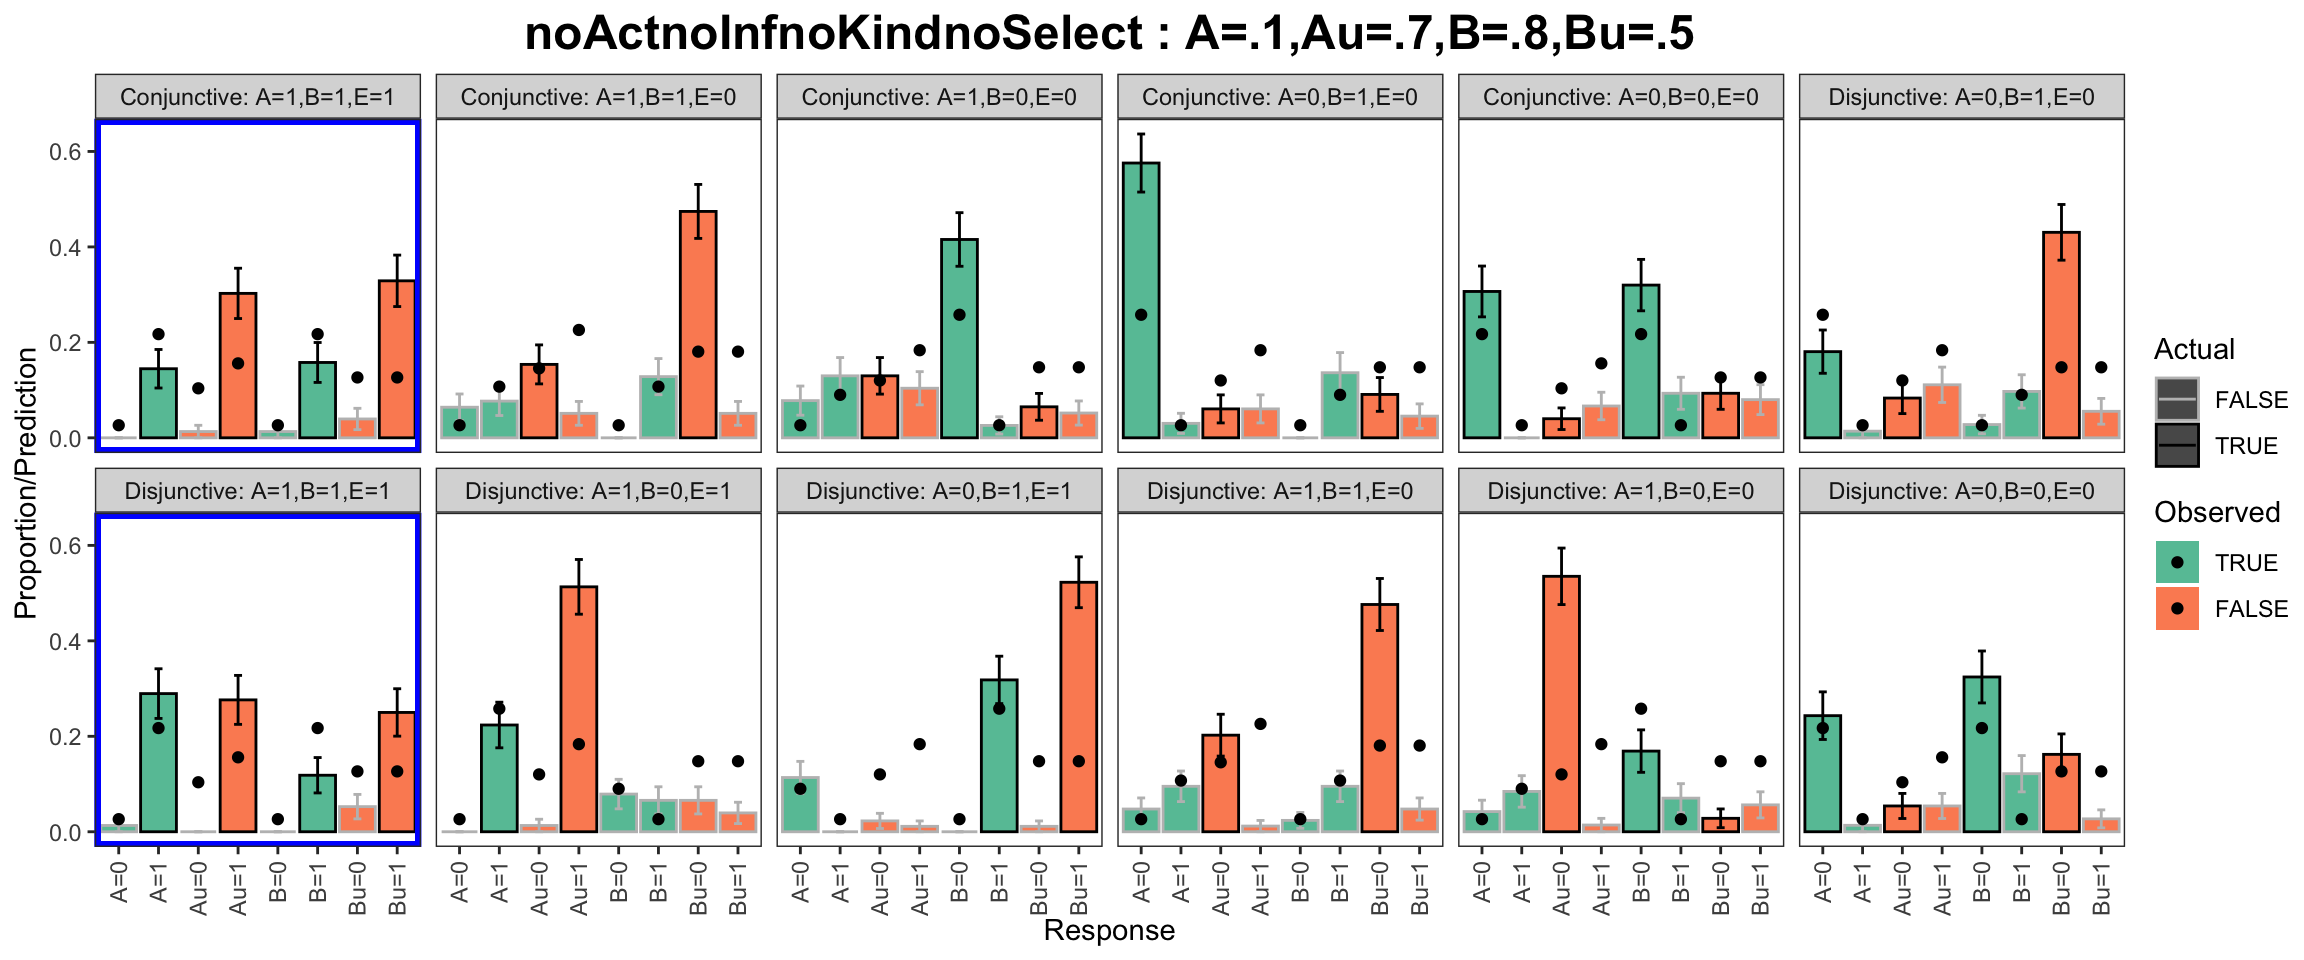
\includegraphics[keepaspectratio]{reportingFigs16m_files/figure-latex/unnamed-chunk-7-48.pdf}}

\end{document}
